\documentclass[../main.tex]{subfiles}
\begin{document}
\section{Critical transitions}\label{sec3}
In the first Chapter we explored how several different EWS have been derived for three different forms of precursors of critical transitions in natural phenomena.
In most of the cited literature the data from which these signals arose came from idealised mathematical models.
This is particularly the case for ecological and climate systems where meaningful real-life data gathering is complex and requires a substantial undertaking in terms of resources.
As a result of this idealisation the quality and robustness of a proposed EWS heavily relies on the accuracy with which such simplified models capture the essence of a phenomenon of interest.
To that end in this Chapter we will devote our attention on how such models are built in an increasingly complex setting.
We will start with the most simple case derived with restrictive assumptions regarding the time-evolution of the systems under investigation and what impact those assumptions have on the prognosis of tipping events.
We will thus evaluate how, as we subsequently drop some of these assumptions, the models become more realistic at the cost of increased complexity in the analysis.
This construction will aid the intuition on how to mathematically investigate catastrophic events in dynamical systems with the aim of understanding how global properties of the model can be exploited in order to predict them.
\subsection{Low-dimensional dynamical systems}\label{subsec3.1}
The naive interpretation of a system exhibiting a critical transition is that the temporal evolution $\dot{x}=f(x)$ of a set of observables $x\in \mathbb{R}^{n}$ undergoes a sudden, qualitative change at particular values of an intrinsic (potentially hidden) parameter $\mu\in \mathbb{R}^{m}$. 
Here the dimensionality of the state space $\mathbb{R}^{n}$ is important to characterise as $n \sim \mathcal{O}(1)\ll\infty$ as it fundamentally enables us to apply classical dynamical systems theory for the discovery of equilibria, (hyperbolic) invariant sets and their bifurcation.
In those low-dimensional systems there are multiple causes that may drive the dynamics to tip towards different regimes (two of which we have already informally introduced in the previous Chapter):
\begin{itemize}
     \item bifurcation-induced (B-tipping): also known as dynamic bifurcations, they are the result of dynamical systems passing through a bifurcation of their parameters causing one or multiple attractors to lose their stability;
     \item rate-induced (R-tipping): when the evolution of a system fails to track the time-changing attractor caused by the rate of change of the parameters rather than their values (as opposed to what happens at bifurcation points);
     \item noise-induced (N-tipping): affecting those systems perturbed by sufficiently high noise which causes the state to depart far enough from a neighbour of a stable equilibrium so that it eventually escapes the basin of attraction.
\end{itemize}
In must be emphasized that given any dynamical system, critical transitions may occur because of one or multiple concurrent causes described above and in general it is not possible to discern the original source of such tipping.
\subsubsection{Deterministic transitions: bifurcation-induced (B-)tipping}\label{subsubsec3.1.1}
In classical dynamical systems, the location (in state space) and the stability of equilibria and their manifolds is studied at fixed values of the parameter $\mu$.
In the context of bifurcation theory in fact the loss of hyperbolicity of these objects may cause the system to undergo a local or global bifurcation which inherently changes the stability or even the existence of the attractors. 
This causes the model's state to shift the dynamical regime from slow stable time-evolution to a fast unstable one.
The theory upon which these systems are investigated has been known since the 1930s\footnote{\url{http://www.scholarpedia.org/article/History\_of\_dynamical\_systems}} and ever since expanded upon to include complex dynamics such as chaos theory and delayed differential equations (DDEs).
However in real-world phenomena it is reasonable to assume that while the system's dynamics dictates the evolution of the observables in phase space at specific parameter values, the system properties also indirectly affect the parameter itself.
Therefore the first assumption to be dropped in our quest of deriving these high-fidelity models is the stationarity of the parameter $\mu$ and the formulation of an augmented (albeit still low-dimensional) version of the original system. 
In the simplest form the time variation of the parameter is monotonic and linear with the ramping characterised by a timescale $\tau:=\varepsilon t$, $0<\varepsilon\ll1$ much slower than that of the observables' dynamics.
The resulting system is therefore called fast-slow
\begin{equation}\label{eq3.1}
   \begin{cases}
           \dot{x}:=\frac{d}{dt}x=f(x;\mu) \,, \\
           \dot{\mu}:=\frac{d}{dt}\mu=\varepsilon \,, 
   \end{cases}\quad \longleftrightarrow\quad
   \begin{cases}
           \newprime{x}:=\frac{d}{d\tau}x=\varepsilon^{-1}f(x;\mu)\,, \\
           \newprime{\mu}:=\frac{d}{d\tau}\mu=1\,,
   \end{cases}
\end{equation}
and it has been the cornerstone object for the development of geometric singular perturbation theory (GSPT) \cite{Wechselberger20}, extensively applied in the analysis of biological mechanisms s.a. calcium cell signaling \cite{Pages19}.
In \cite{Kuehn11} such formulation is the starting point in the discussion of a general and robust framework for the characterisation of critical transitions in low-dimensional systems.
Notably the fast-slow dynamics is approximated by resolving the layer equation
\begin{equation}\label{eq3.2}
   \begin{cases}
           \dot{x}=f(x;\mu) \,, \\
           \dot{\mu}=0 \,, 
   \end{cases}
\end{equation}
which is obtained by taking the singular limit $\varepsilon\to0$ of the system in the fast timescale (i.e. the leftmost system in \eqref{eq3.1}), and the reduced equation
\begin{equation}\label{eq3.3}
   \begin{cases}
      0=f(x;\mu) \,, \\
      \newprime{\mu}=1 \,, 
   \end{cases}
\end{equation}
which is derived via the singular limit of the system in slow timescale (which is the rightmost system in \eqref{eq3.1}).
The centerpiece of the whole analysis is the derivation of the critical manifold $C:=\{(x,\mu)\in \mathbb{R}^{n+m}\;:\;f(x;\mu)=0\}$ as it constraints the solutions of the slow subsystem \eqref{eq3.3} to a unique codim$-m$ object as shown in the following example.
\begin{example}[label=ex3.1]{}{}
     Consider the following $1-$dimensional fast-slow dynamical system
     \begin{equation*}
        \begin{cases}
            \dot{x}(t) = -\mu -x^{2}\,, \\
            \dot{\mu}(t) = \varepsilon \,, 
        \end{cases}
     \end{equation*}
     with the slow parameter $\mu$ varying linearly with the fast timescale $t$. 
     We notice that in the singular limit $\varepsilon\to0$ the fast subsystem gives us exactly the saddle-node normal form for fixed values of $\mu$
     \begin{equation*}
             \dot{x}(t) = -\mu(t) - x^{2}\,,\quad\mu(t)=\mu(0)+\cancelto{0}{\varepsilon}\,t=\mu(0)=:\mu_{0}\,,\;\forall t>0\,.
     \end{equation*}
    To derive the critical manifold we simply compute the equilibria of the layer equation above
    \begin{equation*}\label{eq}
            C=\{(x,\mu)\in \mathbb{R}^{2}\;:\; \mu=-x^{2}\}\,.
    \end{equation*}
\end{example}
\begin{example_continued}
   \begin{figure}[H]
       \centering 
       \begin{subfigure}[b]{0.475\textwidth}
        \centering 
        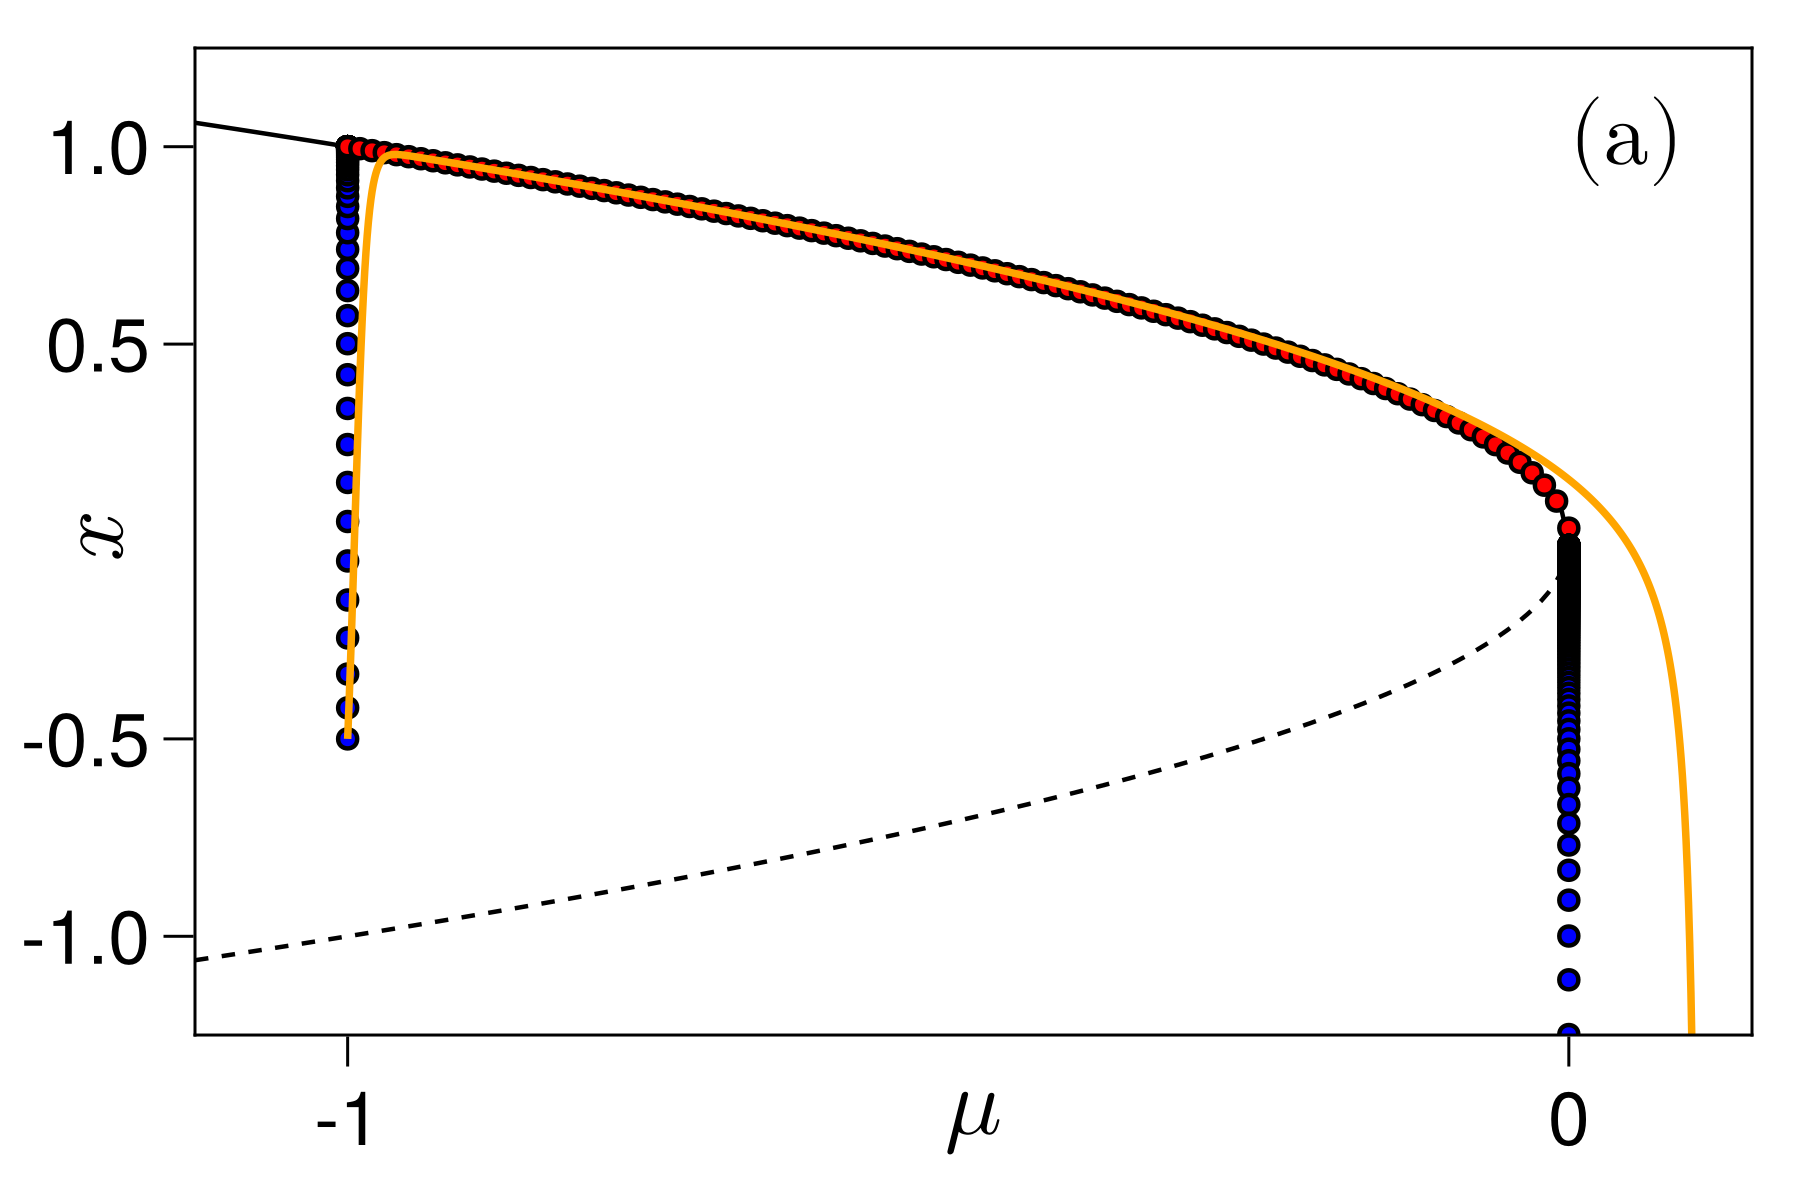
\includegraphics[keepaspectratio, width = \textwidth]{../figures/fig3.1.1.png}
        \label{fig3.1.1}
       \end{subfigure}
       \hfill 
       \begin{subfigure}[b]{0.475\textwidth}
        \centering 
        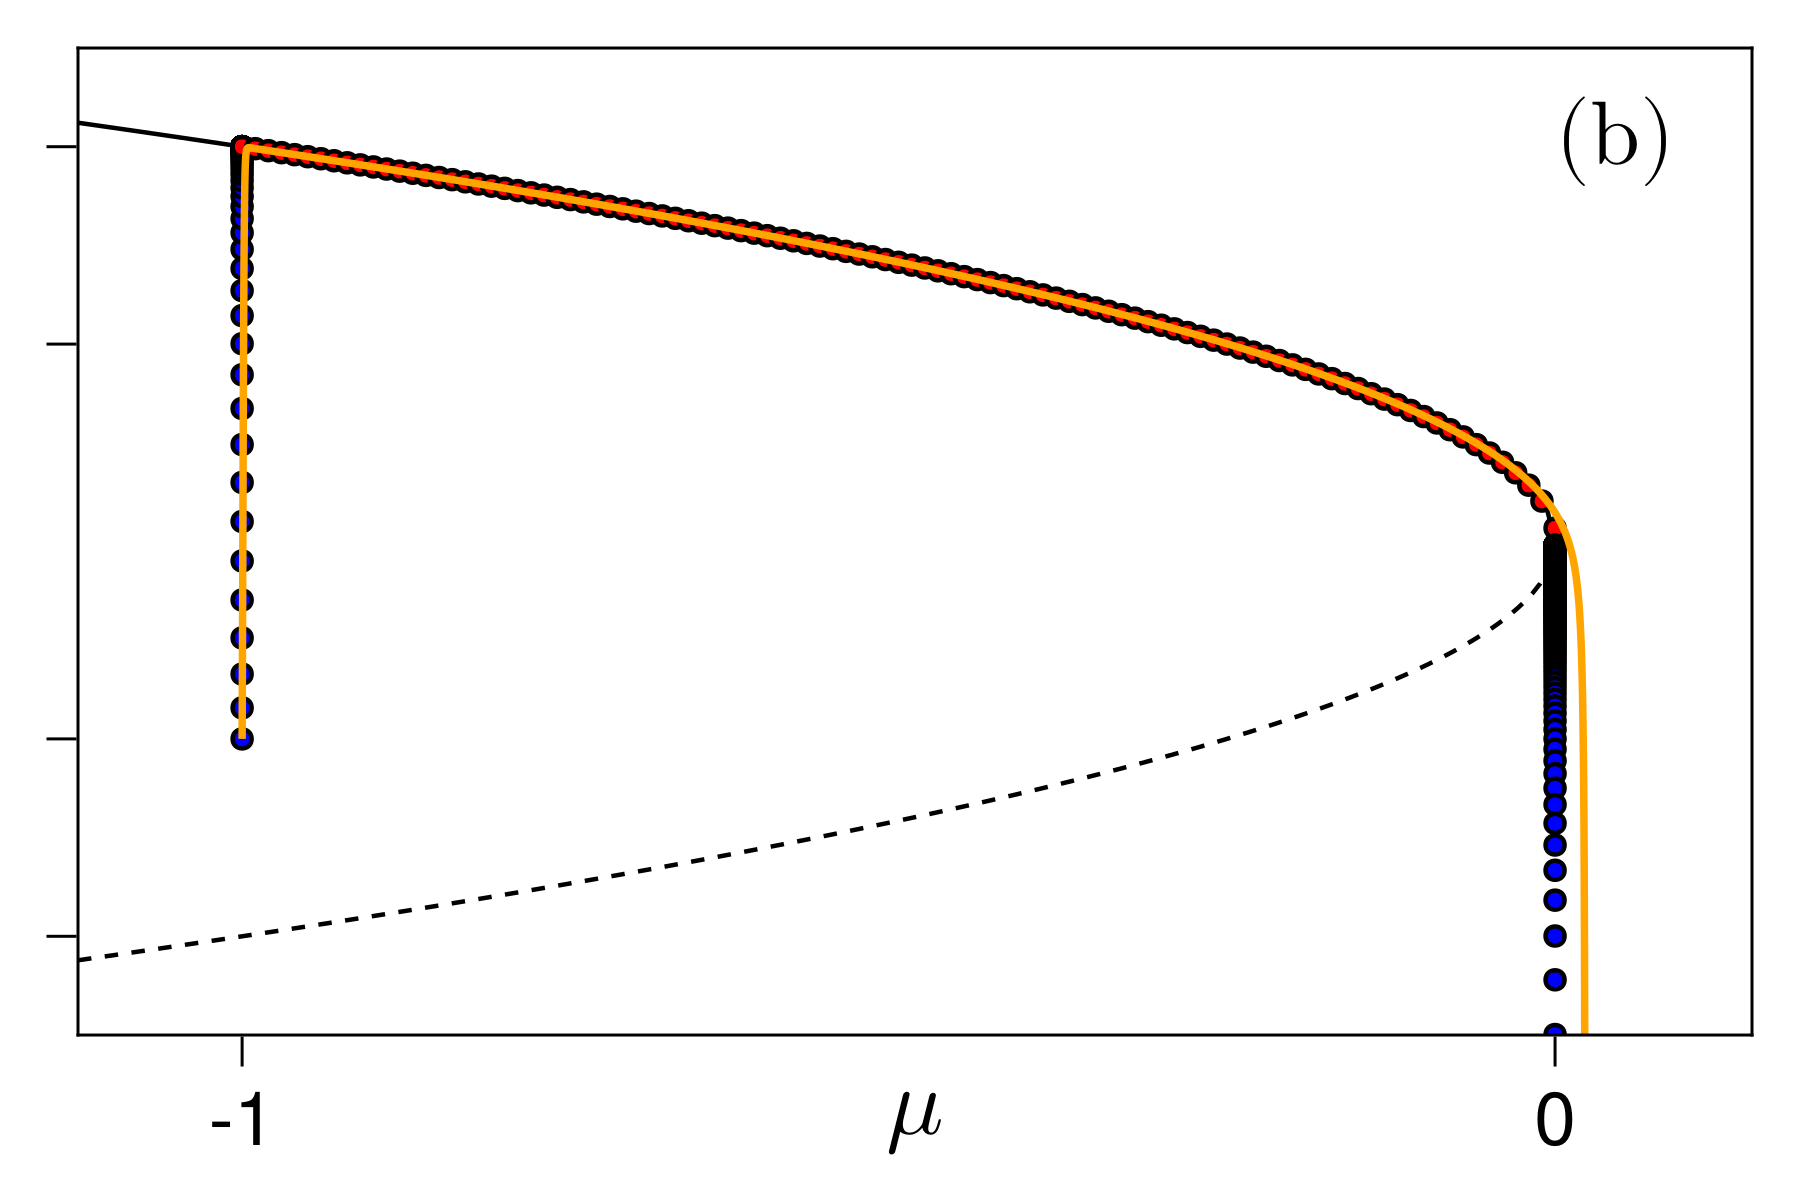
\includegraphics[keepaspectratio, width = \textwidth]{../figures/fig3.1.2.png}
        \label{fig3.1.2}
       \end{subfigure}
       \caption{Comparison of the (numerical) fast-slow trajectory (yellow curve) of the codim$-1$ saddle-node normal form  with different linear rampings ((a): $\varepsilon=10^{-2}$; (b): $\varepsilon=10^{-3}$) and its approximation given by different regimes in the singular limit.
       Solutions of the layer problem \eqref{eq3.2} in blue dots, with initial conditions $(-0.5,-1)$ and $(0,0)$, connected by a solution of the reduced problem \eqref{eq3.3} in red dots with initial condition $(1,-1)$. 
Notice how the dynamics on the critical manifold prescribes the solution of the slow subsystem and the delay of the critical transition in the fast regime is determined by the value of the timescale separation constant $\varepsilon$.}
       \label{fig3.1}
   \end{figure}
\end{example_continued}
An important result from GSPT allows us to characterise a family of (infinitely many) slow manifolds $C_{\varepsilon}:=\{(x,\mu)\in \mathbb{R}^{n+m}\;:\;x=h_{\varepsilon}(\mu)=h(\mu)+\mathcal{O}(\varepsilon)\}$ where $h:\mu\to x$ is given by \ref{thm2.1}.
\begin{theorem}[label=thm3.1]{Fenichel's $(1^{st})$ Theorem}{}
     Let $C$ be a compact, normally hyperbolic manifold then for $\varepsilon>0$ sufficiently small there exists $C_{\varepsilon}$ locally invariant and diffeomorphic to $C$ that lies at a Hausdorff distance $O(\varepsilon)$ from $C$.
\end{theorem}
These singularly perturbed slow manifolds will become paramount later on in the derivation of statistical measure as precursors of critical transitions which we hereby define.
\begin{definition}[Critical transition]\label{def3.1}
     Let $\gamma(t)$ be a homeomorphic image of the real subset $(a,b)$ s.t. for each partitioning ${a=t_{0}<t_1,\dots,t_{N-1}<t_N=b}$ the image $\gamma(t_{j-1},t_j)$ is an orientation preserving trajectory of either the layer \eqref{eq3.2} or the reduced equation \eqref{eq3.3} and let $p\in C$ be a point where the critical manifold loses its hyperbolicity, then $p$ is a critical transition if there exist a candidate trajectory $\gamma$ s.t. $p = \gamma(t_j)$ is a transition between fast and slow regimes and $\gamma(t_{j-1},t_j)$ is hyperbolic and attracting.
\end{definition}
\subsubsection{Different timescales: rate-induced (R-)tipping}\label{subsubsec3.1.2}
The modelling of critical transitions in the fast-slow formulation also introduces an additional mechanism driving the tipping in which the ramping of the parameter is itself the cause of sudden regime shifts in the dynamics. 
In \cite{Ashwin12} the rate of change of $\mu$ is shown to cause, for some specific critical values, sudden regime shifts in the dynamics of a fast-slow system that does not feature a deterministic bifurcation, otherwise known as R-tipping. 
\begin{definition}[]\label{def3.2}
        Let $x\in \mathbb{R}^{n}$ be a state variable, $\mu\in \mathbb{R}$ a time-changing parameter, $R>0$ a constant and $M$ a fixed, stable and invertible linear operator then the linearised system
        \begin{equation*}
             \newprime{x}(t)=M(x-x^{*}(\mu)),
        \end{equation*}
        is said to be (adiabatically) tracking the stable equilibria $x_{\text{eq}}(\mu)$ if $\forall t\;|x(t)-x_{\text{eq}}(\mu(t))|<R$ and viceversa it tips beyond the equilibria if $\exists t_{0}\;\text{s.t.}\;|x(t_0)-x_{\text{eq}}(\mu(t_0))|=R$. 
\end{definition}
The so-called tipping radius $R$ is identified by constructing the condition upon which a fast-slow system fails to track the (slow) drift of the attractor
To study the dependence of the tipping event from the rate of change of the time-varying parameter we formally introduce the drift of the stable equilibria
\begin{equation*}
        r(t):=\frac{d}{dt}(x_{\text{eq}}(\mu(t))) = \frac{dx_{\text{eq}}}{d\mu}\frac{d\mu}{dt} = \varepsilon \frac{dx_{\text{eq}}}{dt}\,.
\end{equation*}
With these quantities defined we are ready to define a criterion for R-tipping for systems with steady drift.
\begin{theorem}[label=thm3.2]{}{}
Let \eqref{eq3.1} be a system with tipping radius $R>0$ and $r(t)=r>0$ is constant (i.e. steady drift of the parameter), then 
\begin{equation*}
          ||M||^{-1}|r|>R
\end{equation*}
is a sufficient condition for R-tipping to occur.
\end{theorem}
\begin{proof}
     Given an initial condition $x(0)=x_{0}$ the general solution of \eqref{eq3.1} is
     \begin{equation*}
         x(t) = e^{Mt}x_{0}+\int_{s=0}^{t}e^{M(t-s)}M\,x_{\text{eq}}(\mu(s))\,ds = - \int_{u=0}^{\infty}e^{Mu}M\,x_{\text{eq}}(\mu(t-u))\,du\,,
     \end{equation*}
     where the dependence on the initial condition is dropped from the second integral by assuming an arbitrarly long past while setting $u:=t-s$. Integrating by parts the general solution gives us
     \begin{equation*}
             x(t) = -[e^{Mu}x_{\text{eq}}(\mu(t-u))]_{0}^{\infty} - \int_{0}^{\infty}e^{Mu}\frac{d}{dt}(x_{\text{eq}}(\mu(t-u)))\,du\:\Rightarrow\: x(t) - x_{\text{eq}}(\mu(t)) = -\int_{0}^{\infty}e^{Mu}r(\mu(t-u))\,du\,,
     \end{equation*}
     where the (exponential) stability of the linear operator $(|e^{Mt}\to0|\;\text{as}\; t\to \infty)$ has been used. We integrate by parts again and obtain 
     \begin{equation*}
         x(t) - x_{\text{eq}}(\mu(t)) = M^{-1}r(\mu(t-u))-\int_{0}^{\infty}e^{Mu}M^{-1}\,\newprime{r}(\mu(t-u))\,du\,.
     \end{equation*}
     Assuming now steady drift the above simplifies to
     \begin{equation*}
         x(t) - x_{\text{eq}}(\mu(t)) = M^{-1}r\;\Rightarrow\;|x(t) - x_{\text{eq}}(\mu(t))| = |M^{-1}r|\,.
     \end{equation*}
     By choosing the matrix norm for the linear operator $||M||=\text{sup}_{v\neq0}\frac{|Mv|}{|v|}$ then it trivially follows
     \begin{equation*}
         ||M||^{-1}|r|\leq|M^{-1}r|\leq||M^{-1}|||r|\,.
     \end{equation*}
     We now recall from Definition \ref{def3.2} the condition for R-tipping which gives us the sufficient condition $||M||^{-1}|r|>R$ for the solution to slip off the stable equilibria thereby causing the rate-induced critical transition.
\end{proof}
This result allows us to generalise the analysis to systems that have no known deterministic bifurcations therefore dropping the additional constraint of restricting ourselves to problems that can be recast in a normal form.
\begin{example}[label=ex3.2]{}{}
As an example we consider the following $2-$dimensional model of compost-bomb instability \cite{Wieczorek11} in the slow timescale
\begin{equation*}
        \begin{cases}
            \varepsilon \newprime{x} = y + \mu + x(x-1)\,, \\
            \newprime{y} = - x - x^2 - x^{3} - x^{4} - x^{5}\,,
        \end{cases}
\end{equation*}
with steady (linear) ramping of the parameter $\mu\in \mathbb{R}$.
The system has one stable equilibrium at $(0,-\mu)$ and in the singular limit we are able to derive the critical manifold 
\begin{equation*}
            C=\{(x,y)\in \mathbb{R}^{2}\;:\;y=-\mu-x(x-1)\}\,,
\end{equation*}
with attracting $C^{(a)}=\{C\cap\{x<\frac{1}{2}\}\}$ and repelling $C^{(r)}=\{C\cap\{x>\frac{1}{2}\}\}$ submanifolds separated by a saddle line which is tangent to $C$ along $x=\frac{1}{2}$. Note that the distance along $x$ between the stable equilibrium and the fold of the critical manifold is exactly $\frac{1}{2}=R$ which will thus provide us the tipping radius for our system.
We now differentiate the critical manifold w.r.t. the slow timescale to obtain
\begin{align}
        0 =&\;\dot{x} + \dot{\mu} + \frac{d}{d\tau}(x^{2}-x) = f_{2}(x, y) + r + \dot{x}(2x-1)\;\Rightarrow \nonumber \\
        \Rightarrow&\;\dot{x}=-\frac{f_{2}(x, y)+r}{2x-1} \,, \label{eq3.4}
\end{align}
where we have $f_{2}(x, y):=\dot{y}=- x - x^{2} - x^{3} - x^{4} - x^{5} = -\sum_{n=1}^{5}x^{\,n}$ for the slow dynamics as well as the definition for the drif $\dot{\mu} =: r$.
We immediately realise that \eqref{eq3.4} is singular along the fold of the critical manifold therefore, by recalling that $\tau = \epsilon t\;\Rightarrow\;\frac{dt}{d\tau}=\epsilon^{-1}$, we shift the temporal framework onto the fast timescale $t$ obtaining
\begin{equation}\label{eq3.5}
   \begin{cases}
      \newprime{x} = r - \sum_{n=1}^{5}x^{n}  \,, \\
      \newprime{\mu} = -r(2x-1) \,, 
   \end{cases}
\end{equation}
The equilibria for \eqref{eq3.5} will finally give us the (parametrised) invariant set of $x$ points to which trajectories starting within the attracting submanifolds will converge to
\begin{equation*}
        M(r) = \{(x, y)\in \mathbb{R}^{2}\;:\;\sum_{n=1}^{5}x^{n}=r\}
\end{equation*}
To find the critical value $r_{c}$ for the drift of the parameter that causes the state to tip and slip off the critical manifold we only need to substitute the value for the tipping radius previously derived in $M(r)$ which thus gives us $r_{c}\approx 0.9687$.
We conclude that drift values $r>r_{c}$ will move the invariant set over and across the fold of the critical manifold meaning that even those trajectories that start within $C^{(a)}$ will slip off the stable equilibria and tip in a rate-induced critical transition.
\end{example}
\begin{example_continued}
\begin{figure}[H]
    \centering 
    \begin{subfigure}[b]{0.485\textwidth}
        \centering 
        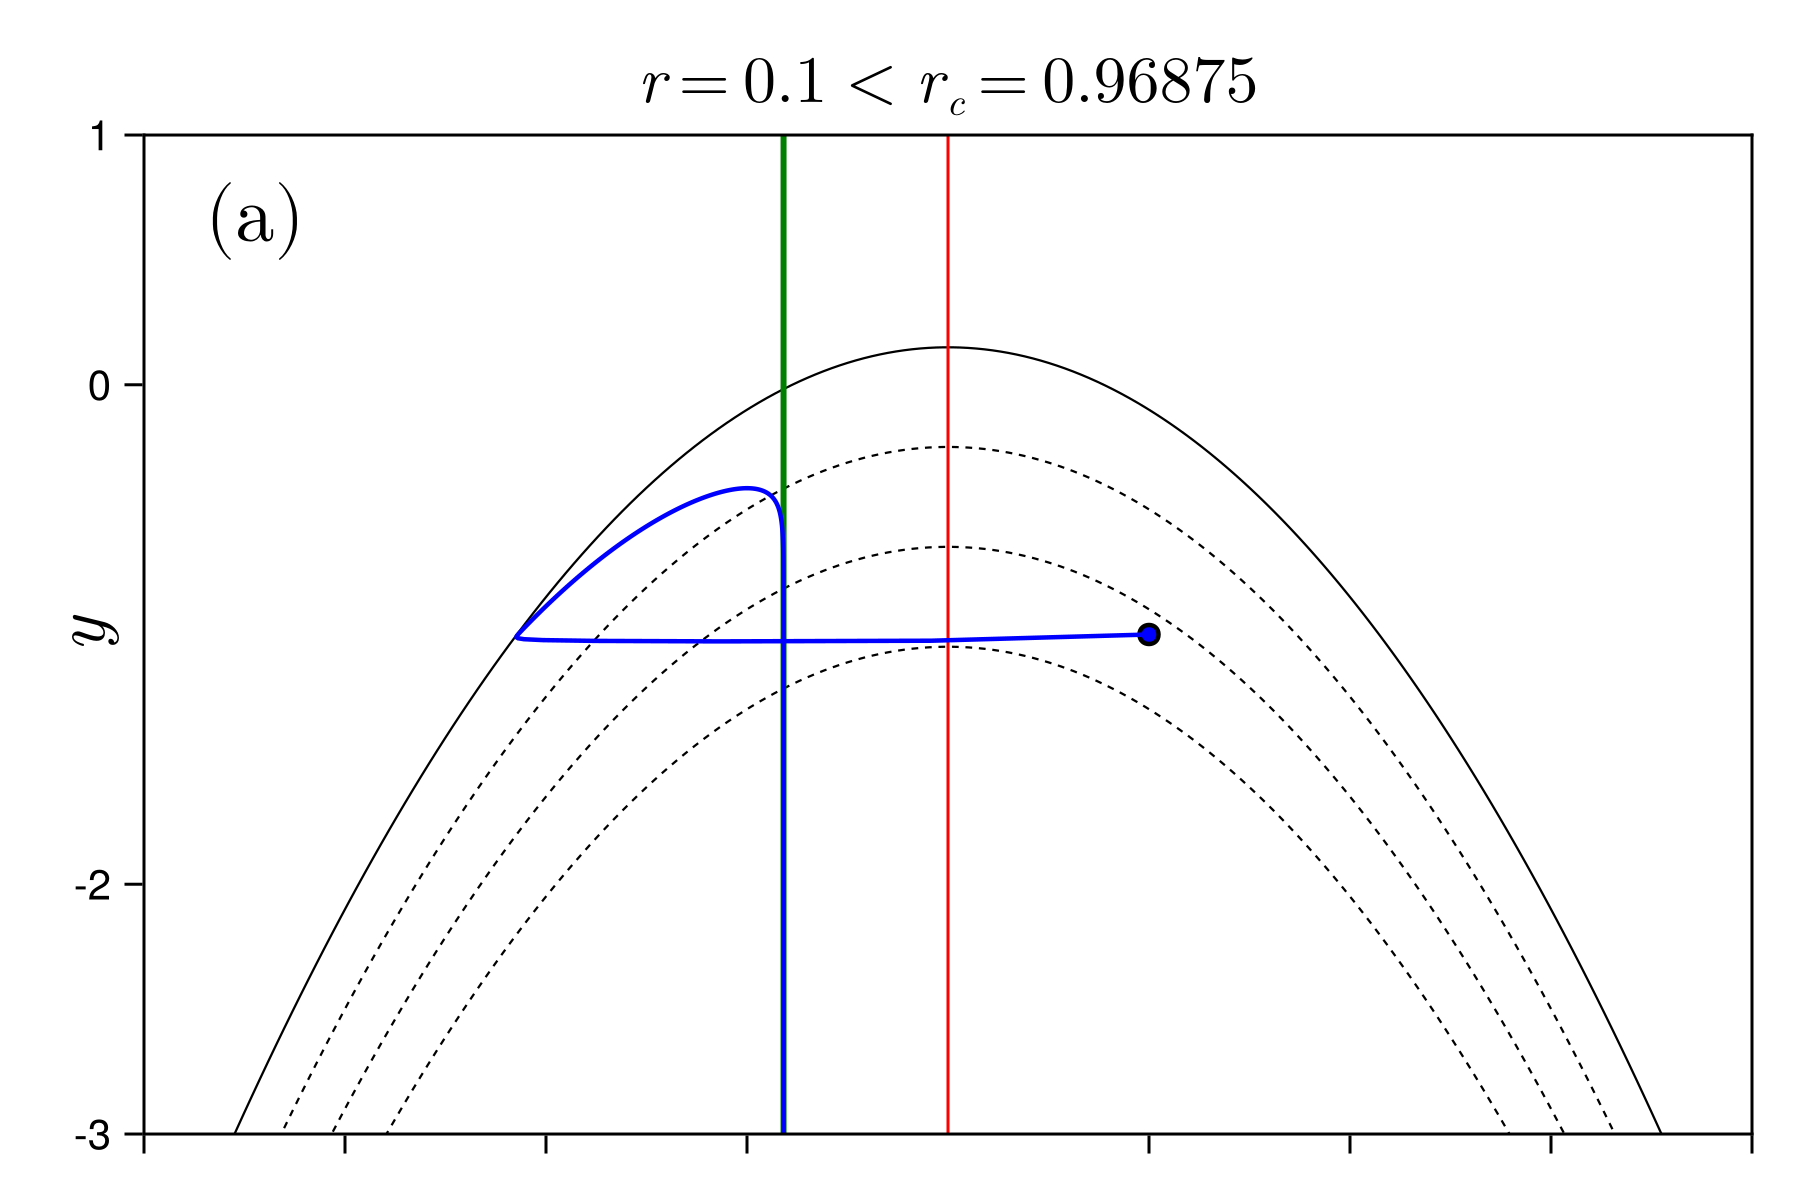
\includegraphics[keepaspectratio, width = \linewidth]{../figures/fig3.2.1.png}
        \label{fig3.2.1}
    \end{subfigure}
    \hfill 
    \begin{subfigure}[b]{0.485\textwidth}
        \centering 
        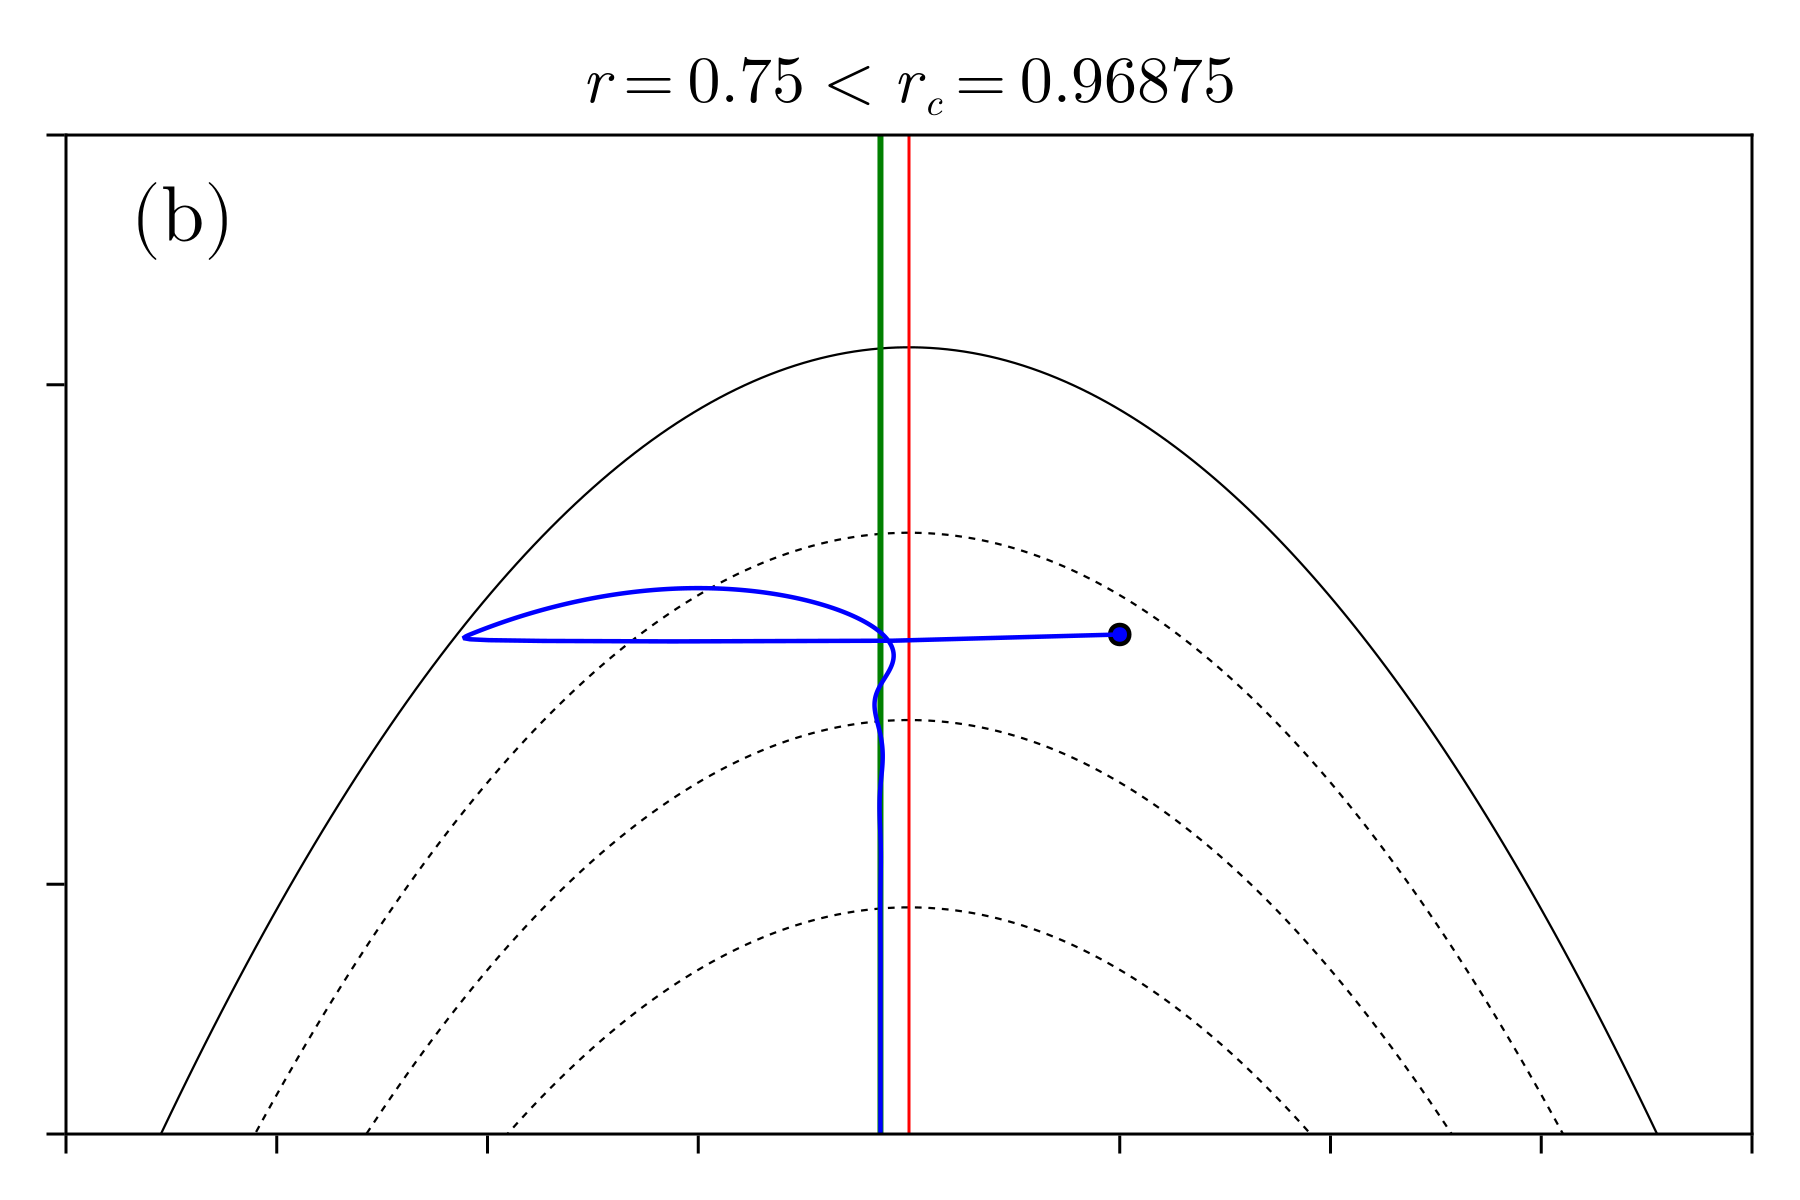
\includegraphics[keepaspectratio, width = \linewidth]{../figures/fig3.2.2.png}
        \label{fig3.2.2}
    \end{subfigure}


    \begin{subfigure}[b]{0.485\textwidth}
        \centering 
        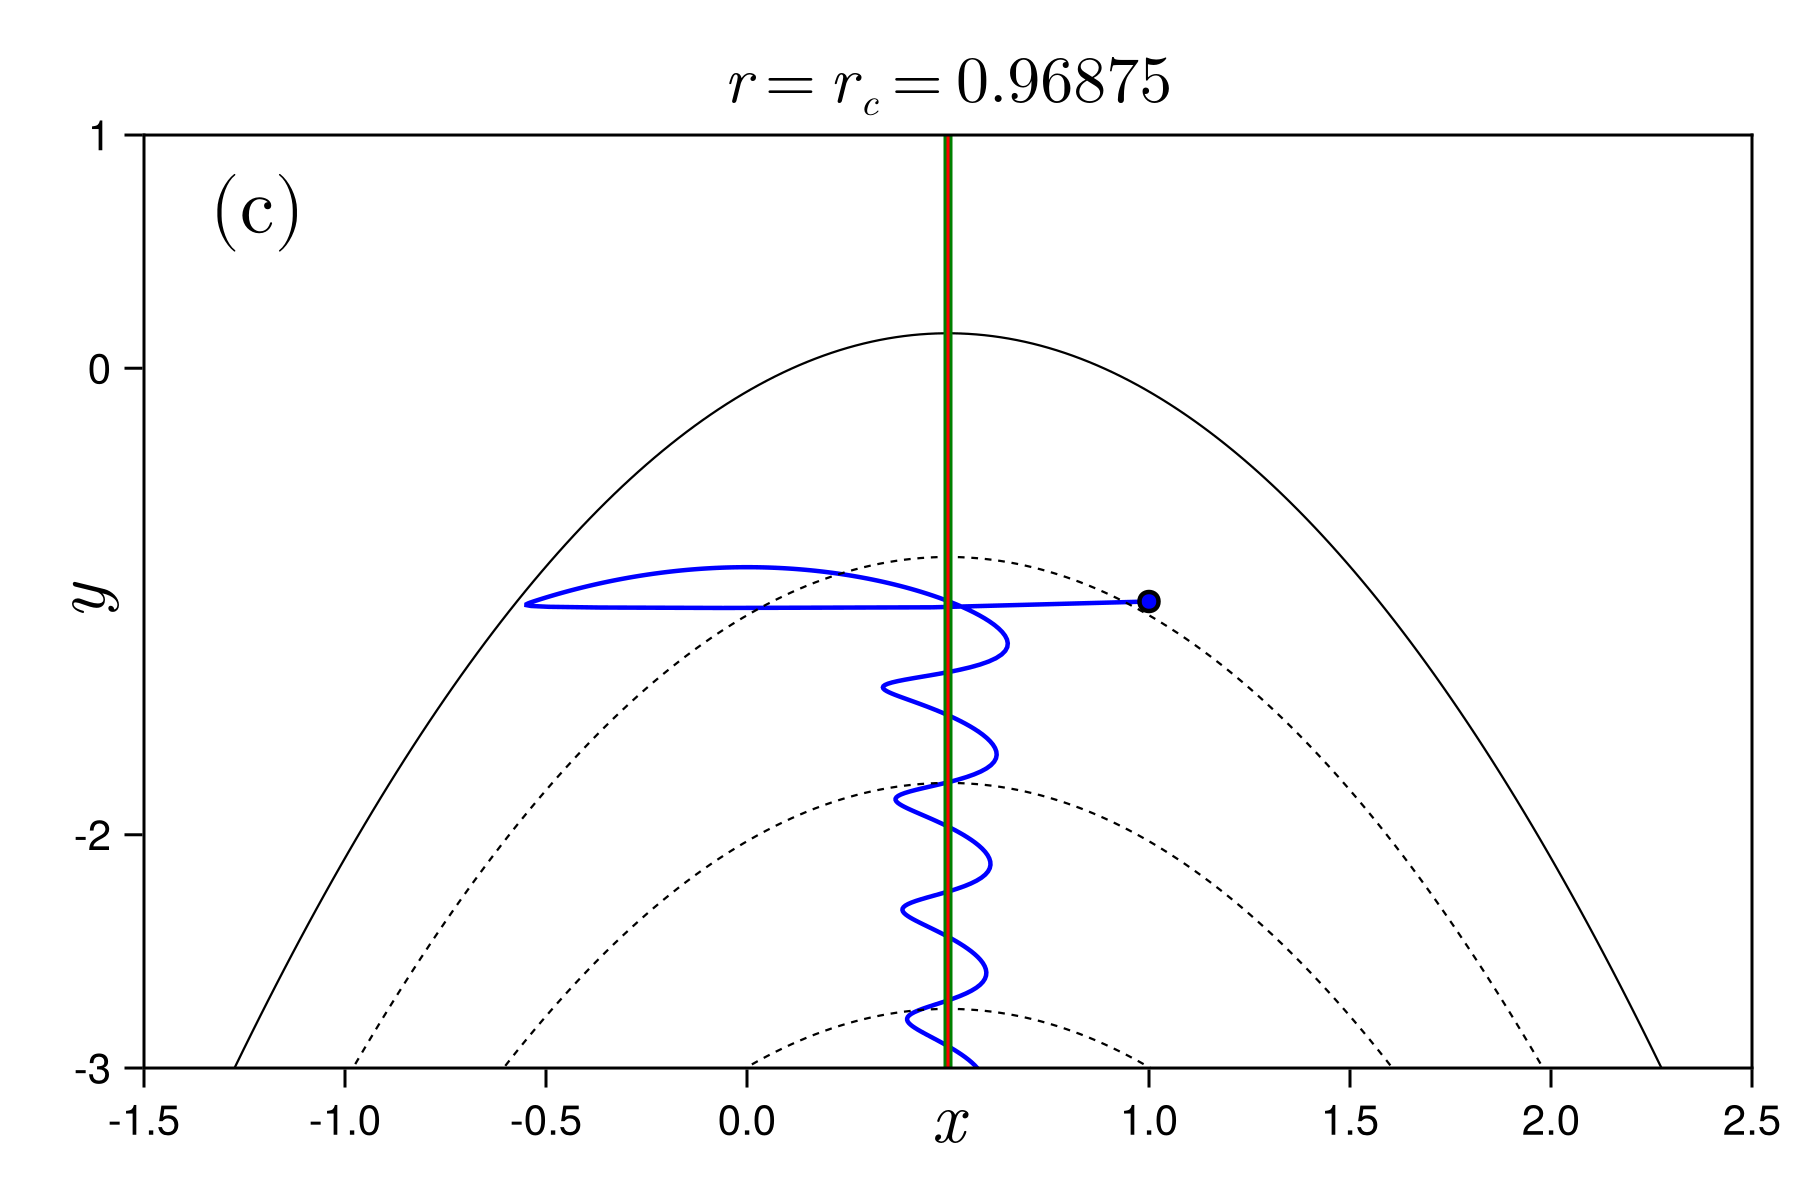
\includegraphics[keepaspectratio, width = \linewidth]{../figures/fig3.2.3.png}
        \label{fig3.2.3}
    \end{subfigure}
    \hfill
    \begin{subfigure}[b]{0.485\textwidth}
        \centering 
        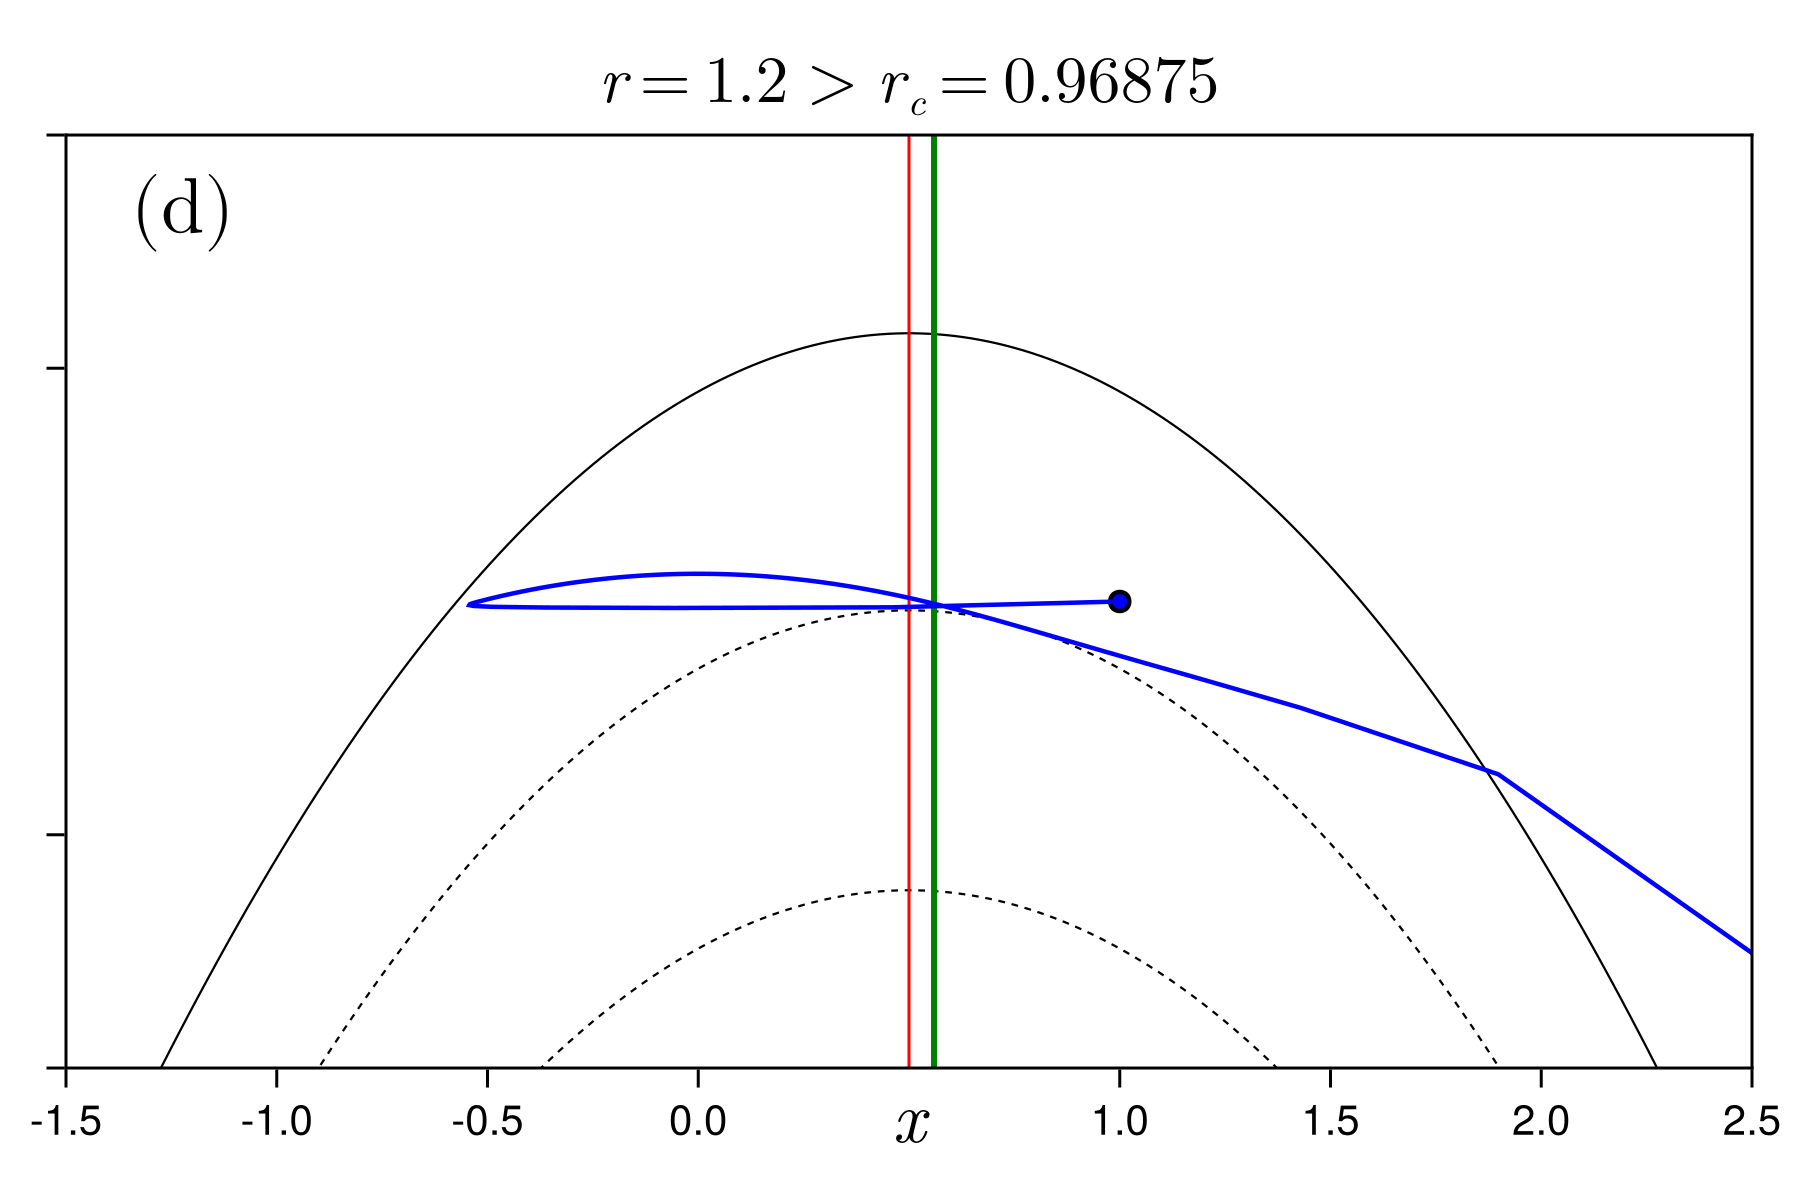
\includegraphics[keepaspectratio, width = \linewidth]{../figures/fig3.2.4.png}
        \label{fig3.2.4}
    \end{subfigure}
    \caption{Forward-time trajectories (blue curves) of the compost-bomb fast-slow system propagated from the IC $(1,-1)$ (blue dots) located in the inner part of the attracting submanifold $C^{(a)}$ with timescale separation value $\varepsilon = 2\cdot10^{-2}$ and parameter $\mu$ varied linearly in $[0,2]$ at different rates $r(t)$.
            Notice how as we keep increasing the drift of the parameter while keeping it below the critical value (a)$\sim$(b) the invariant set (solid red line) moves closer to the fold of the critical manifold (here depicted as the solid black curve for the initial parameter value of $\mu=0.1$ and as dashed black curves at increasing parameter values) but never crosses it, allowing the trajectories to eventually settle on the invariant set (solid green lines) meaning that they will remain close (within tipping radius distance) to the stable equilibrium. 
    For a drift corresponding to the critical value $r_{c}$ (c) we notice large oscillations while the trajectories try to settle along the invariant set which has now moved over and overlapping with the saddle.
Finally as we keep increasing the drift over the critical value (d) we clearly see that now the invariant line as crossed over the fold and thus the trajectories are now unable to track the stable equilibrium thereby slipping off the critical manifold.}
    \label{fig3.2}
\end{figure} 
\end{example_continued}
As mentioned in the description of Figure \ref{fig3.1} the non-stationarity of the parameter implies a delay in the tipping event. 
As such a natural question arises in how this delay reflects in the detection of EWS of R-tipping events. 
In 2016 Ritchie and colleagues \cite{Ritchie16} observed that an increase in variance and autocorrelation also feature the same delay w.r.t. the critical parameter drift value and analytically characterised it for a saddle-node normal form.
6 years later in 2023 Ritchie et al. \cite{Ritchie23} revisited this concept for more complex settings of predator-prey ecological systems and the possible collapse of the Atlantic meridional overturning circulation (AMOC), both with non-linear ramps of the forcing parameter.
The same climate model was used 2 years prior \cite{Lohmann21} to conclude how R-tipping could in principle lead to a cascading effect of tipping points predicted by an increase in variance and autocorrelation.
\subsubsection{Stochastic perturbations: noise-induced (N-)tipping}\label{subsubsec3.1.3}
One substantially strong assumption that we need to discard in order to build a more realistic dynamical system for the prediction of critical transition is the deterministic character of its dynamics.
Whether it is due to the intrinsic stochastic nature of the phenomenon under investigation or to the noise naturally embedded in the sensory data collected in scientific monitoring, the stochastic character of real-world timeseries data is inevitable.
We thus need to move away from the classical theory of flows in ordinary differential equations (ODEs) and into the realm of stochastic processes.
In \cite{Kuehn11} the fast-slow problem \eqref{eq3.1} in the slow timescale $\tau=\varepsilon t$ is reformulated as an Itô differential form
\begin{equation}\label{eq3.6}
   \begin{cases}
      dx = \epsilon^{-1} f(x;\mu)d\tau + \frac{\sigma_f}{\sqrt{\epsilon}}\,dW\,, \\
      d\mu = g(x;\mu)d\tau\,, 
   \end{cases}
\end{equation}
whith $f$ and $g$ modelling the deterministic drift of an ensemble's average of trajectories, $\sigma_{f}$ modelling the stochastic diffusion on such ensemble and $W$ representing Brownian motion.
We can now exploit the slow manifold $C_{\varepsilon}$ introduced in Theorem \ref{thm3.1} to derive a criterion to discern an ensemble's trajectory close to the critical transition from one that is in a stable regime.
According to Definition \ref{def3.1} in fact, a sample path of an ensemble of trajectories of \eqref{eq3.6} that stays close (in probabilistic terms) to $C_{\varepsilon}$ will be in a regime of slow, stable evolution.
It is thus intuitive to define a new stochastic process $\xi(\tau)=x(\tau)-h_{\epsilon}(\mu)$ which quantifies the statistical departure of the sample path $x(\tau)$ from the critical manifold. 
We then apply Ito's formula to this new process to derive the associated SDE; after that we define once again a new stochastic process $X(\tau):=\sigma_f^{-2} \text{Var}(\xi)$ which satisfies the following deterministic fast-slow system
\begin{equation}\label{eq3.7}
   \begin{cases}
      \dot{X} = 2\epsilon^{-1}A_{\epsilon}(\mu)X +1 \,, \\
      \dot{\mu} = g(h_{\epsilon}(\mu),\mu) \,, 
   \end{cases}
\end{equation}
with $A_{\epsilon}(\mu)=(D_x f)(h_{\epsilon}(\mu),\mu) - \epsilon (D_{\mu} h_{\epsilon})(\mu) (D_x g)(h_{\epsilon}(\mu),\mu)$. 
Applying Theorem \ref{thm3.1} again for \eqref{eq3.7} we can construct a new slow manifold for the sample paths of the new stochastic fast-slow system
\begin{equation}\label{eq3.8}
        C_{\epsilon}^{(X)}:=\bigg\{(X,\mu)\in \mathbb{R}^2\;:\;X=H_{\epsilon}(\mu):=- \frac{1}{2A_{\epsilon}(\mu)+O(\epsilon)}\bigg\}\,,
\end{equation}
and from that we finally can define a neighbour of the slow manifold which scales with the variance of sample paths
\begin{equation}\label{eq3.9}
        N_{\rho}(C_{\epsilon}):=\bigg\{(x,\mu)\in \mathbb{R}^{2}\;:\;\frac{(x-h_{\epsilon}(\mu))^{2}}{H_{\epsilon}(\mu)}<\rho^2\bigg\}\,.
\end{equation}
We formalise the above derivation in the Theorem below.
\begin{theorem}[label=thm3.4]{}{}
        Let \eqref{eq3.6} be a scalar stochastic fast-slow system (i.e. $n=m=1$) with additive noise (i.e. $\sigma_{f}(x)=\sigma\in \mathbb{R}$) and 
     \begin{equation*}
             N_{\rho}(C_{\varepsilon}):=\bigg\{(x,\mu)\in \mathbb{R}^{2}\;:\;-\frac{(x-h_{\varepsilon}(\mu))^{2}}{2A_{\varepsilon}(\mu)+\mathcal{O}(\varepsilon)}<\rho^2\bigg\}\,,\quad A_{\varepsilon}(\mu)=(D_x f)(h_{\varepsilon},\mu) - \varepsilon (D_{\mu} h_{\varepsilon}) (D_x g)(h_{\varepsilon},\mu)\,,
     \end{equation*}
     be a neighbour of the singularly perturbed slow manifold, then if a sample path has an initial condition on the slow manifold $C_{\varepsilon}$ it will stay bounded within $N_{\rho}(C_{\varepsilon})$ with high probability.
\end{theorem}
Arguably of greater importance for the context of EWS detection is the corollary that follows.
\begin{corollary}
     Since the measure of $N_{\rho}(C_{\varepsilon})$ scales with the variance of $\xi(\tau)$ (which coincides with the variance of $x(\tau)$ from trivial properties of the variance of a sum of stochastic processes) then an increase in the variance implies the neighbour to grow bigger.
\end{corollary}
Whenever a stochastic process tracking a (deterministic) slow stable manifold is \textit{kicked-off} due to the perturbations of the noise and escapes the basin of attraction we are presented with a case of the previously discussed N-tipping.
Despite the notorious difficulty of anticipating N-tipping events, the corollary above provides us with a robust mathematical characterisation of either CSD or flickering through the increase in variance of a stochastic process approaching B-tipping.
The intuition behind CSD for B-tipping is that as the bifurcation is approached the neighbor $N_{\rho}(C_{\varepsilon})$, in which the realisations of the stochastic process are bounded, increases in size allowing for more probability to a N-tipping event to occur.
\begin{example}[label=ex3.3]{}{}
In \cite{Kuehn11} an example is provided to validate this result using an OUP
\begin{equation}\label{eq3.10}
   \begin{cases}
           dx = -\varepsilon^{-1}\alpha x d\tau + \frac{\sigma}{\sqrt{\varepsilon}}dW \,, \\
      d\mu = d\tau \,, 
   \end{cases}
\end{equation}
as benchmark.
Let us consider a sample path realised by the OUP in \eqref{eq3.10} with drift constant $\alpha=1$, timescale constant $\epsilon=2\cdot10^{-2}$ and noise level $\sigma=0.1$.
We want to construct the neighborhood $N_{\rho}(C_{\varepsilon})$ and confirm that the numerical sample paths stay in fact bounded within such neighborhood with high probability. 
To do so we must first construct the (deterministic) slow manifold $C_{\varepsilon}$ and for that we need in turn to derive the map $h_{\varepsilon}(\mu)=h(\mu)+\mathcal{O}(\varepsilon)$.
With the critical manifold coinciding with the $x=0$ axis 
\begin{equation*}
            C=\{(x,\mu)\in \mathbb{R}^{2}\;:\;f(x,\mu)=-\alpha x = 0\:\Rightarrow\: x=0\;\forall \alpha\neq0,\,\forall \mu\in \mathbb{R}\}\,,
\end{equation*}
we can easily check that the existance of $h:\mu\mapsto x$ is guranteed by Theorem \ref{thm2.1} given that $C$ is normally hyperbolic at any point.
It follows similarly that the only map $x=h(\mu)=0,\:\forall \mu\in \mathbb{R}$ is the null function yielding 
\begin{equation*}
                h_{\varepsilon}(\mu) = h(\mu) + \mathcal{O}(\varepsilon) = \mathcal{O}(\varepsilon)\quad\Longrightarrow\quad C_{\varepsilon}=\{(x,\mu)\in \mathbb{R}^{2}\;:\;x=O(\varepsilon)\}\,.
\end{equation*}
This tells us that the slow manifold is a narrow strip wrapped around the critical manifold whose width is twice the Hausdorff distance from $C$.
The next step in our construction is to derive a new slow manifold $C_{\varepsilon}^{(X)}$ for the process 
\begin{equation*}
             X=\sigma^{-2}\text{Var}(\xi)=\sigma^{-2}\text{Var}(x - h_{\varepsilon}(\mu))=\sigma^{-2}\text{Var}(x)\,,
\end{equation*}
where we recall the invariance of the variance under additive constant perturbations.
First we compute the quantity $A_{\epsilon}(\mu)=(D_x f)(h_{\varepsilon}(\mu),\mu) - \varepsilon (D_{\mu} h_{\varepsilon})(\mu) (D_x g)(h_{\varepsilon}(\mu),\mu)=-\alpha$ and then by using the definition
\begin{equation*}
     C_{\varepsilon}^{(X)}:=\bigg\{(X,\mu)\in \mathbb{R}^2\;:\;X=H_{\varepsilon}(\mu):=- \frac{1}{2A_{\varepsilon}(\mu)+\mathcal{O}(\varepsilon)}\bigg\}\,,
\end{equation*}
we get
\begin{equation*}
     C_{\varepsilon}^{(X)}=\{(X,\mu)\in \mathbb{R}^{2}\;:\;X=\frac{1}{2 \alpha}+O_{1}(\varepsilon)\}\,.
\end{equation*}
Furthermore from the definition
\begin{equation*}
     N(\rho;C_{\varepsilon}):=\bigg\{(x,\mu)\in \mathbb{R}^{2}\;:\;\frac{(x-h_{\varepsilon}(\mu))^{2}}{H_{\varepsilon}(\mu)}<\rho^2\bigg\}\,,
\end{equation*}
\end{example}
\begin{example_continued}
we get
\begin{equation}\label{eq3.11}
                N(\rho;C_{\varepsilon})=\bigg\{\frac{\sigma^{-2}\text{Var}(x)+O_{2}(\varepsilon)}{\frac{1}{2 \alpha}+O_{1}(\varepsilon)}<\rho^{2}\bigg\}=\bigg\{\frac{\sigma^{-2}\text{Var}(x)+M_{2}\varepsilon}{\frac{1}{2 \alpha}+M_{1}\varepsilon}<\rho^{2}\bigg\}\,,
\end{equation}
for which $M_{1}, M_{2}$ are two distinct, positive constants that need to be quantified in order to compute $\rho$ which will give us the boundaries $\partial N(\rho;C_{\varepsilon})=\sqrt{\rho^{2}}$.
To do so let us observe that $X=H_{\varepsilon}(\mu)=\frac{1}{2A_{\varepsilon}(\mu)}+O_{1}(\varepsilon)\;\Rightarrow\;|X|=|\sigma^{-2}\text{Var}(x)|< M_{1}\varepsilon$.
We recall that $x(\tau)$ is in fact an OUP for which we have an analytical expression for its variance readily available
\begin{equation}\label{eq3.12}
             \text{Var}(x(\tau)) = \bigg(x_0 - \frac{\sigma^2}{2 \alpha}\bigg)e^{-2\frac{\alpha\tau}{\varepsilon}}\,.
\end{equation}
We can the plug in the values for $\alpha,\,\sigma$ and $\varepsilon$ in \eqref{eq3.12} to get $M_{1}=225$.
Similarly for the other constant we get $x=h_{\varepsilon}(\mu)=O_{2}\;\Rightarrow\;|x|<M_{2}\varepsilon$; here we assume that $\underset{\tau\in \mathbb{R}^{+}}{\text{max}}|x(\tau)|=0.25$ which lead us to the value $M_{2}=12.5$. Putting all together into \eqref{eq3.11} finally gives us $\rho = \pm 0.35$.
We are now able to compute the closure of the neighborhood $N(\rho;C_{\varepsilon})$ of the critical manifold $C_{\varepsilon}$ within which our sample paths $x(\tau)$ for the OUP (which are normally distributed) will stay bounded with high probability.
\begin{figure}[H]
         \centering 
         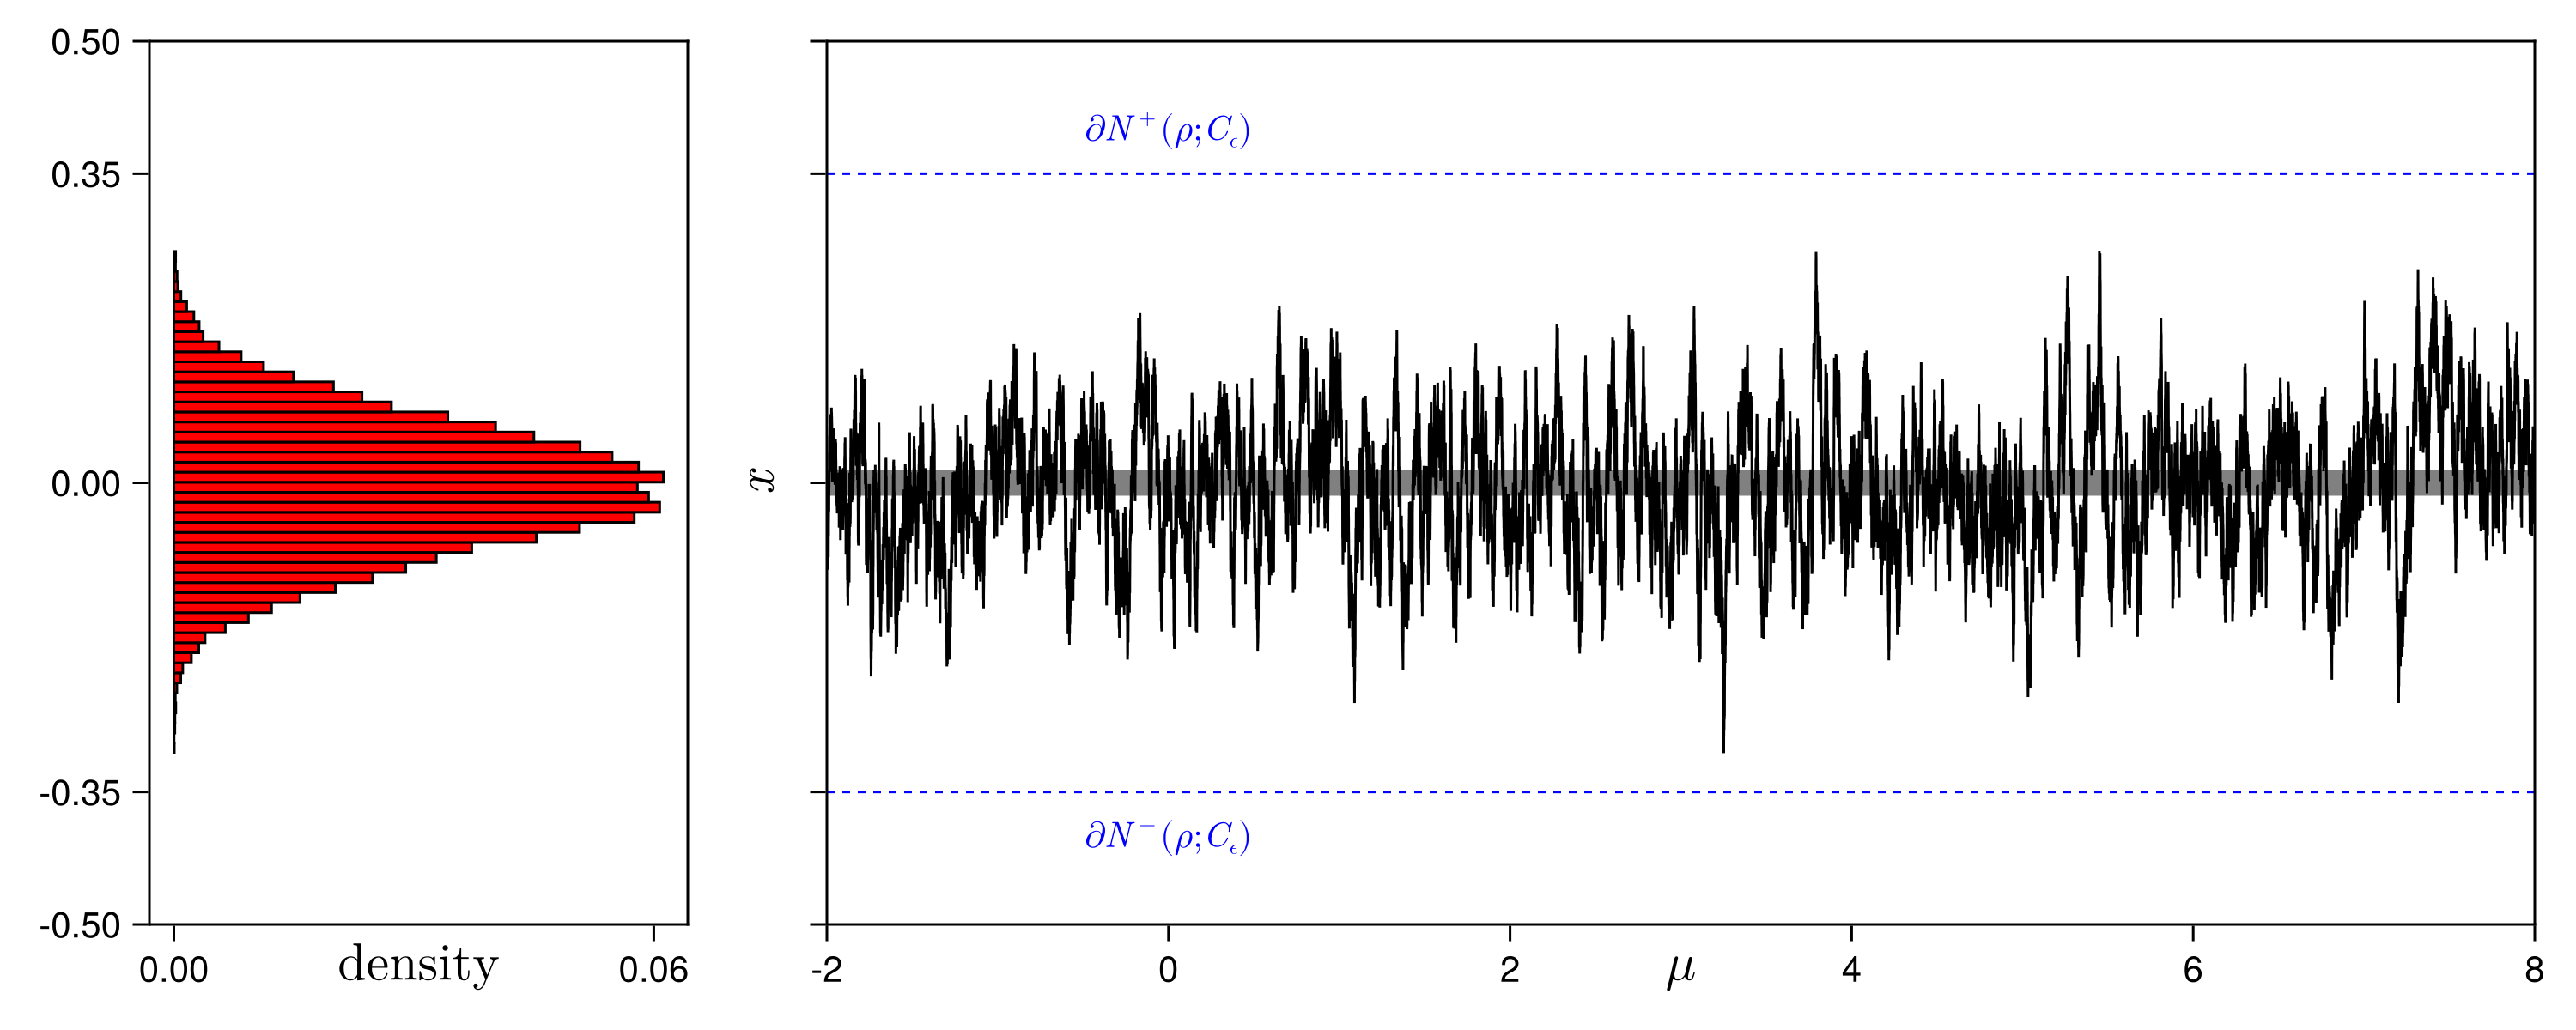
\includegraphics[keepaspectratio, width=\textwidth]{../figures/fig3.3.png}
         \caption{States distribution (left) of a sample path (right) of the OUP \eqref{eq3.10}, with drift $\alpha=1$, timescale separation $\varepsilon=2\cdot10^{-2}$ and noise level $\sigma=0.1$, starting on the slow manifold $C_{\varepsilon}$ (gray strip). 
         Note how the states stay bounded within the neighborhood $N_{\rho}(C_{\varepsilon})$ (dashed blue lines) with probability $1$.}
         \label{fig3.3}
\end{figure}
\end{example_continued}
To substantiate the result given by the corollary we can generalise the approach in detecting CSD through the increase in variance of a sample path of the fast-slow problem by computing the moments of the probability distribution solving the Fokker-Planck equation (FPE) associated to the SDE.
Considering \eqref{eq3.9} again for the case of additive noise, the FPE reads
\begin{equation}\label{eq3.13}
     \partial_{t}p(x,t) = -\partial_{x}J(x,t)\,,\quad J(x,t):= f(x;\mu)p(x,t) - \frac{\sigma^{2}}{2}\partial_{x}p(x,t) \,,
\end{equation}
where $J(x,t)$ is the probability density current.
The fundamental assumption of the analysis carried in \cite{Kuehn11} is that there exist an asymptotic steady-state $x_{s}$ whose distribution $p_{s}(x):=p(x_{s},t)$ satisfies the stationary limit of \eqref{eq3.13} i.e. $\newprime{J}(x) = 0\;\Rightarrow\; J(x) = \text{constant}(x)$. 
We immediately realise that equation \eqref{eq3.13} is defined over the entirety of the real (spatial) domain, meaning that in order to restrict it to a bounded and limited subinterval $[a,b]\subset \mathbb{R}$ we must enforce the entirety of the probability current to never leave such domain, resulting in the specification of reflecting boundary conditions. 
The reason for this immediately follow by the constraint of the stationary Fokker-Planck density to remain normalised in any subdomain $[a,b]$ we restrict ourselves to.
Following the imposition of reflecting boundary conditions we get that the only possible constant that satisfies \eqref{eq3.13} is $J(x)=J=0$. From the definition of $J(x,t)$ this leads to a first-order, homogeneous, non-linear ODE whose general integral can be explicitly calculated
\begin{equation}\label{eq3.14}
     p_{s}(x)=\frac{1}{N}\,e^{2 \int_{a}^{x}\sigma^{-2}f(y;\mu)dy}\,,\quad N = \int_{a}^{b}\int_{a}^{z}\sigma^{-2}f(y;\mu)dy\,dz\,.
\end{equation}
We can now analytically derive the variance from \eqref{eq3.14} for simple forms of the drift $f(x;\mu)$. In \cite{Kuehn11} this is done for the saddle-node, transcritical and subcritical pitchfork normal forms and we compare those with the ensemble variance of $1000$ sample paths as reported in Figure \ref{fig3.5}.
One clear observation that we can gather from Figure \ref{fig3.5} is that in all three cases the (analytic) variance is non-monotonic and it reaches a local maxima in the proximity of the bifurcation at $\mu=0$ before decreasing. 
This apparent anomaly is a result of imposing reflecting boundary conditions for the probability current.
As we previously established in fact, the approach of a critical transition implies that the stationary density $p_{s}(x)$ becomes less confined around the stable equilibrium leading to N-tipping to occur with higher and higher probability.
\begin{figure}[H]
    \centering 
    \begin{subfigure}[b]{0.3\textwidth}
        \centering 
        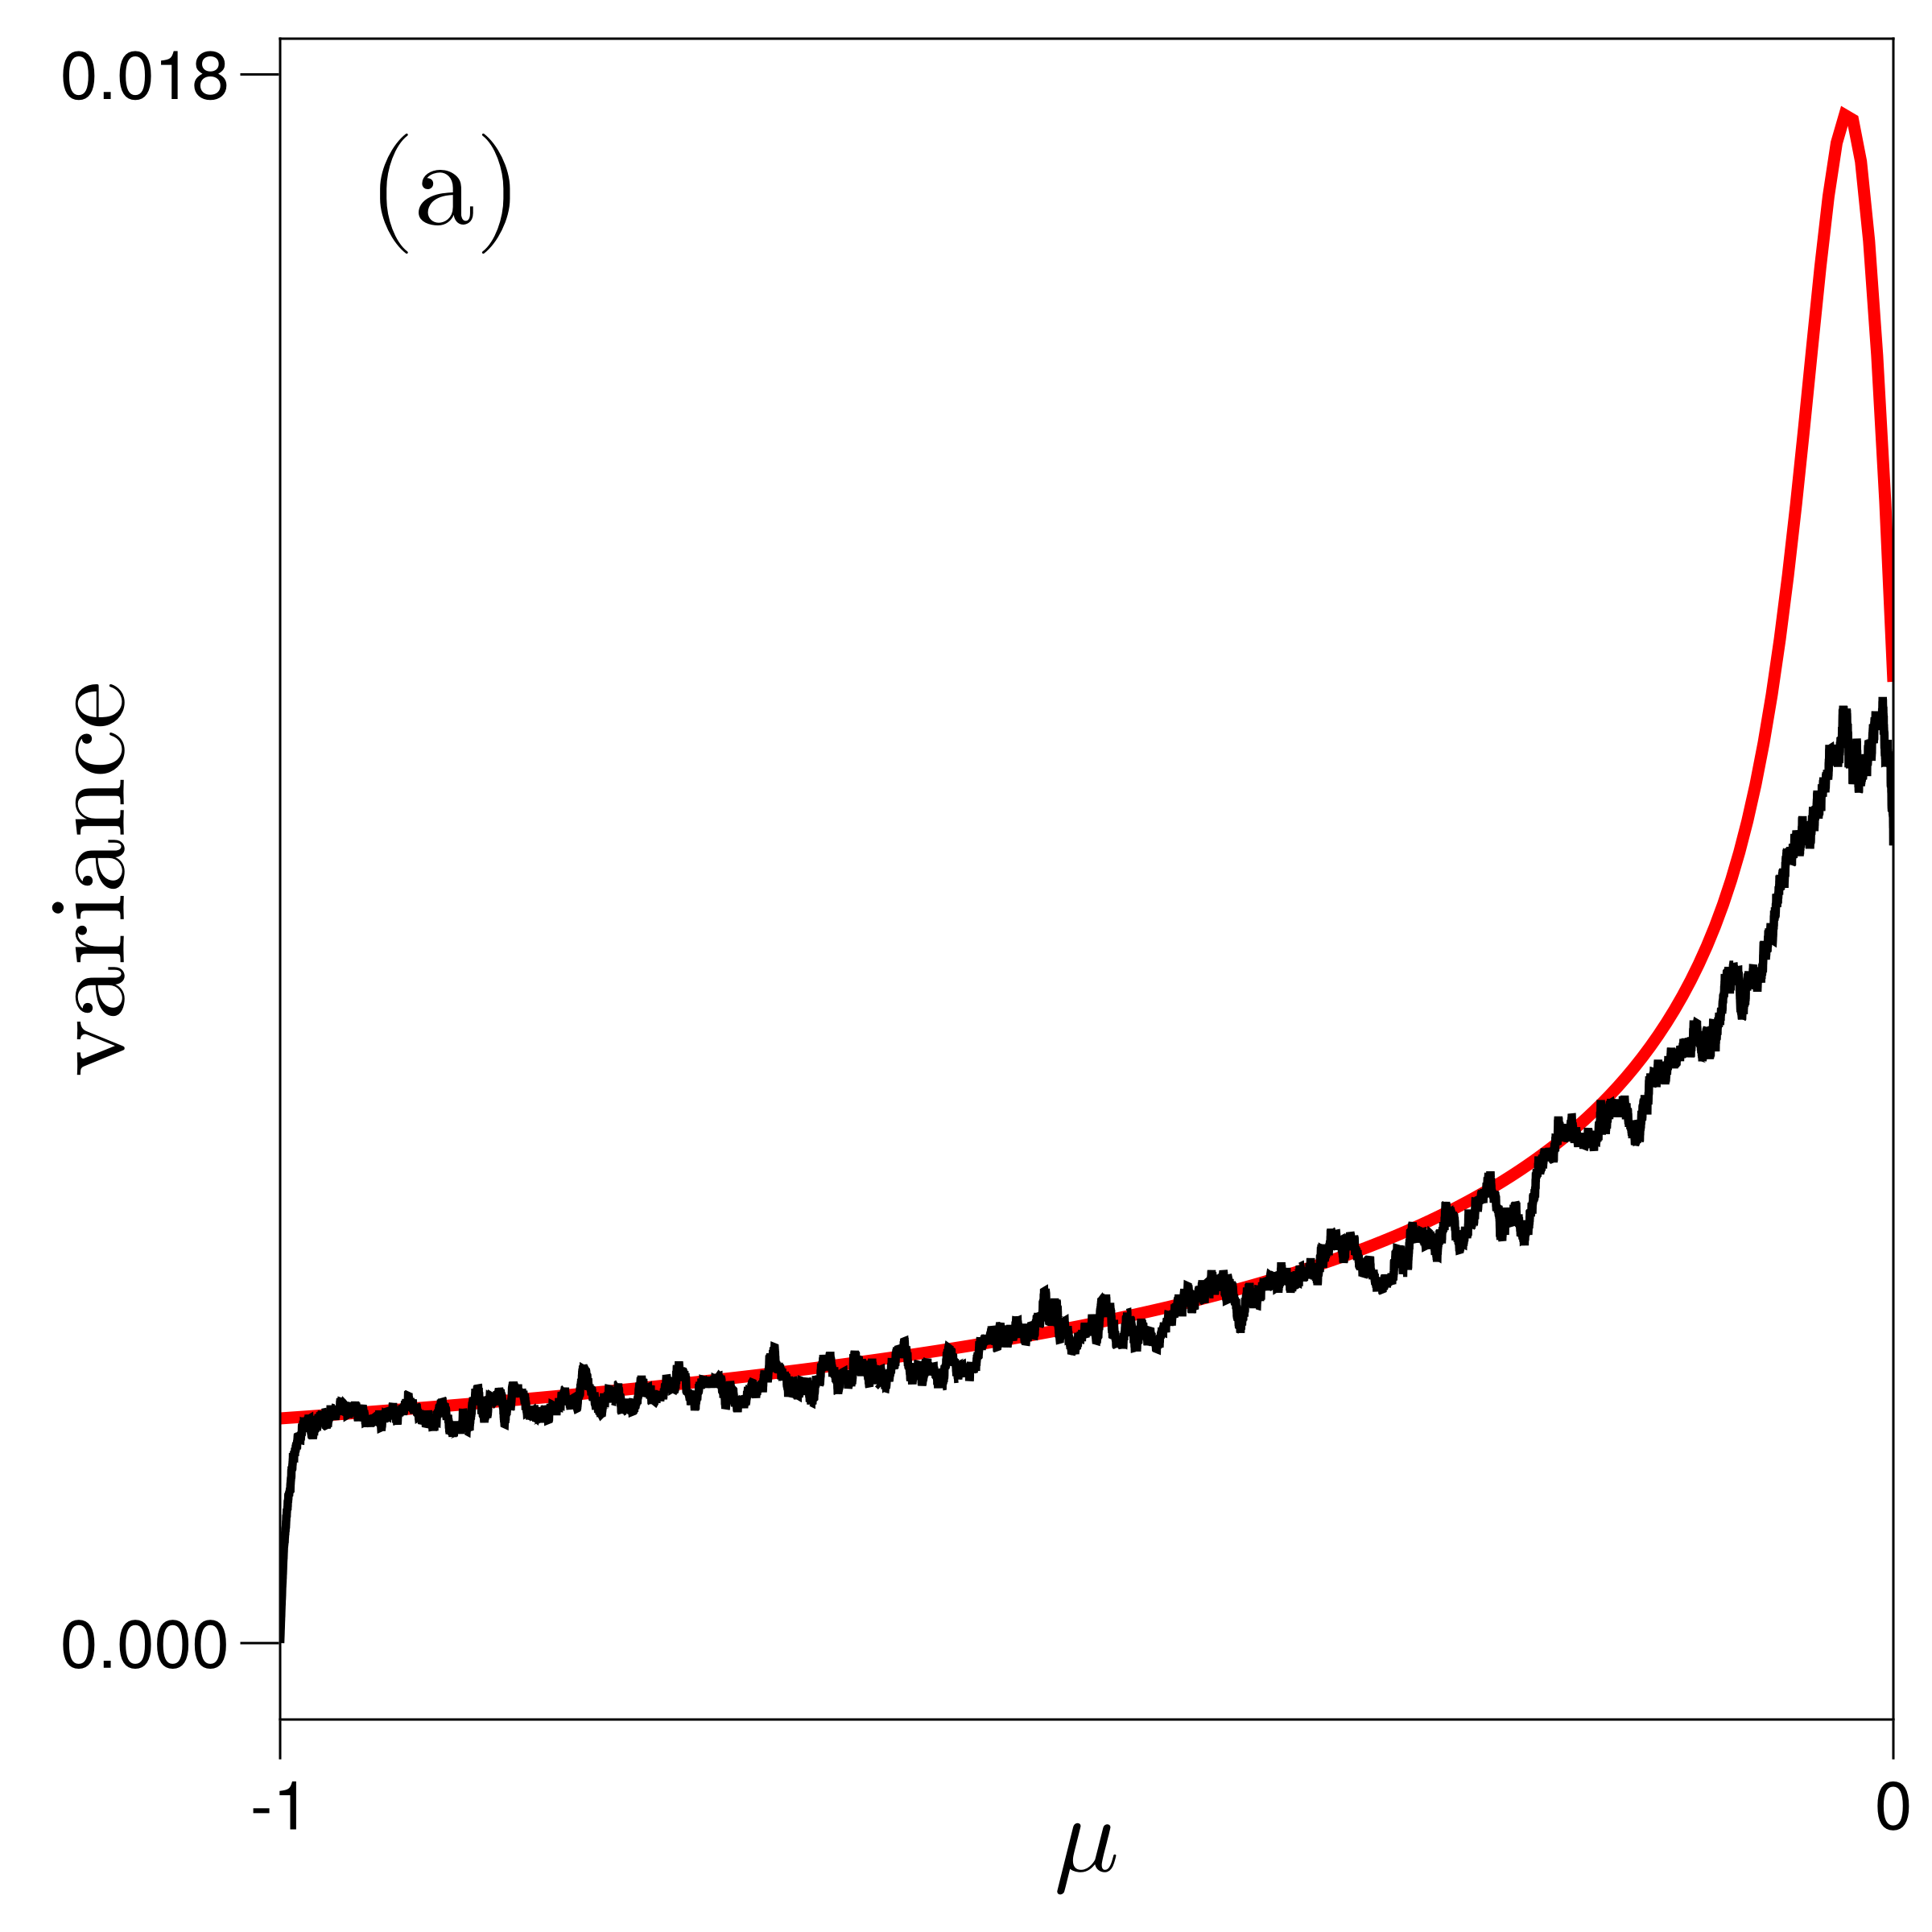
\includegraphics[keepaspectratio, width = \textwidth]{../figures/fig3.5.1.png}
        \label{fig3.5.1}
    \end{subfigure}
    \hfill 
    \begin{subfigure}[b]{0.3\textwidth}
        \centering 
        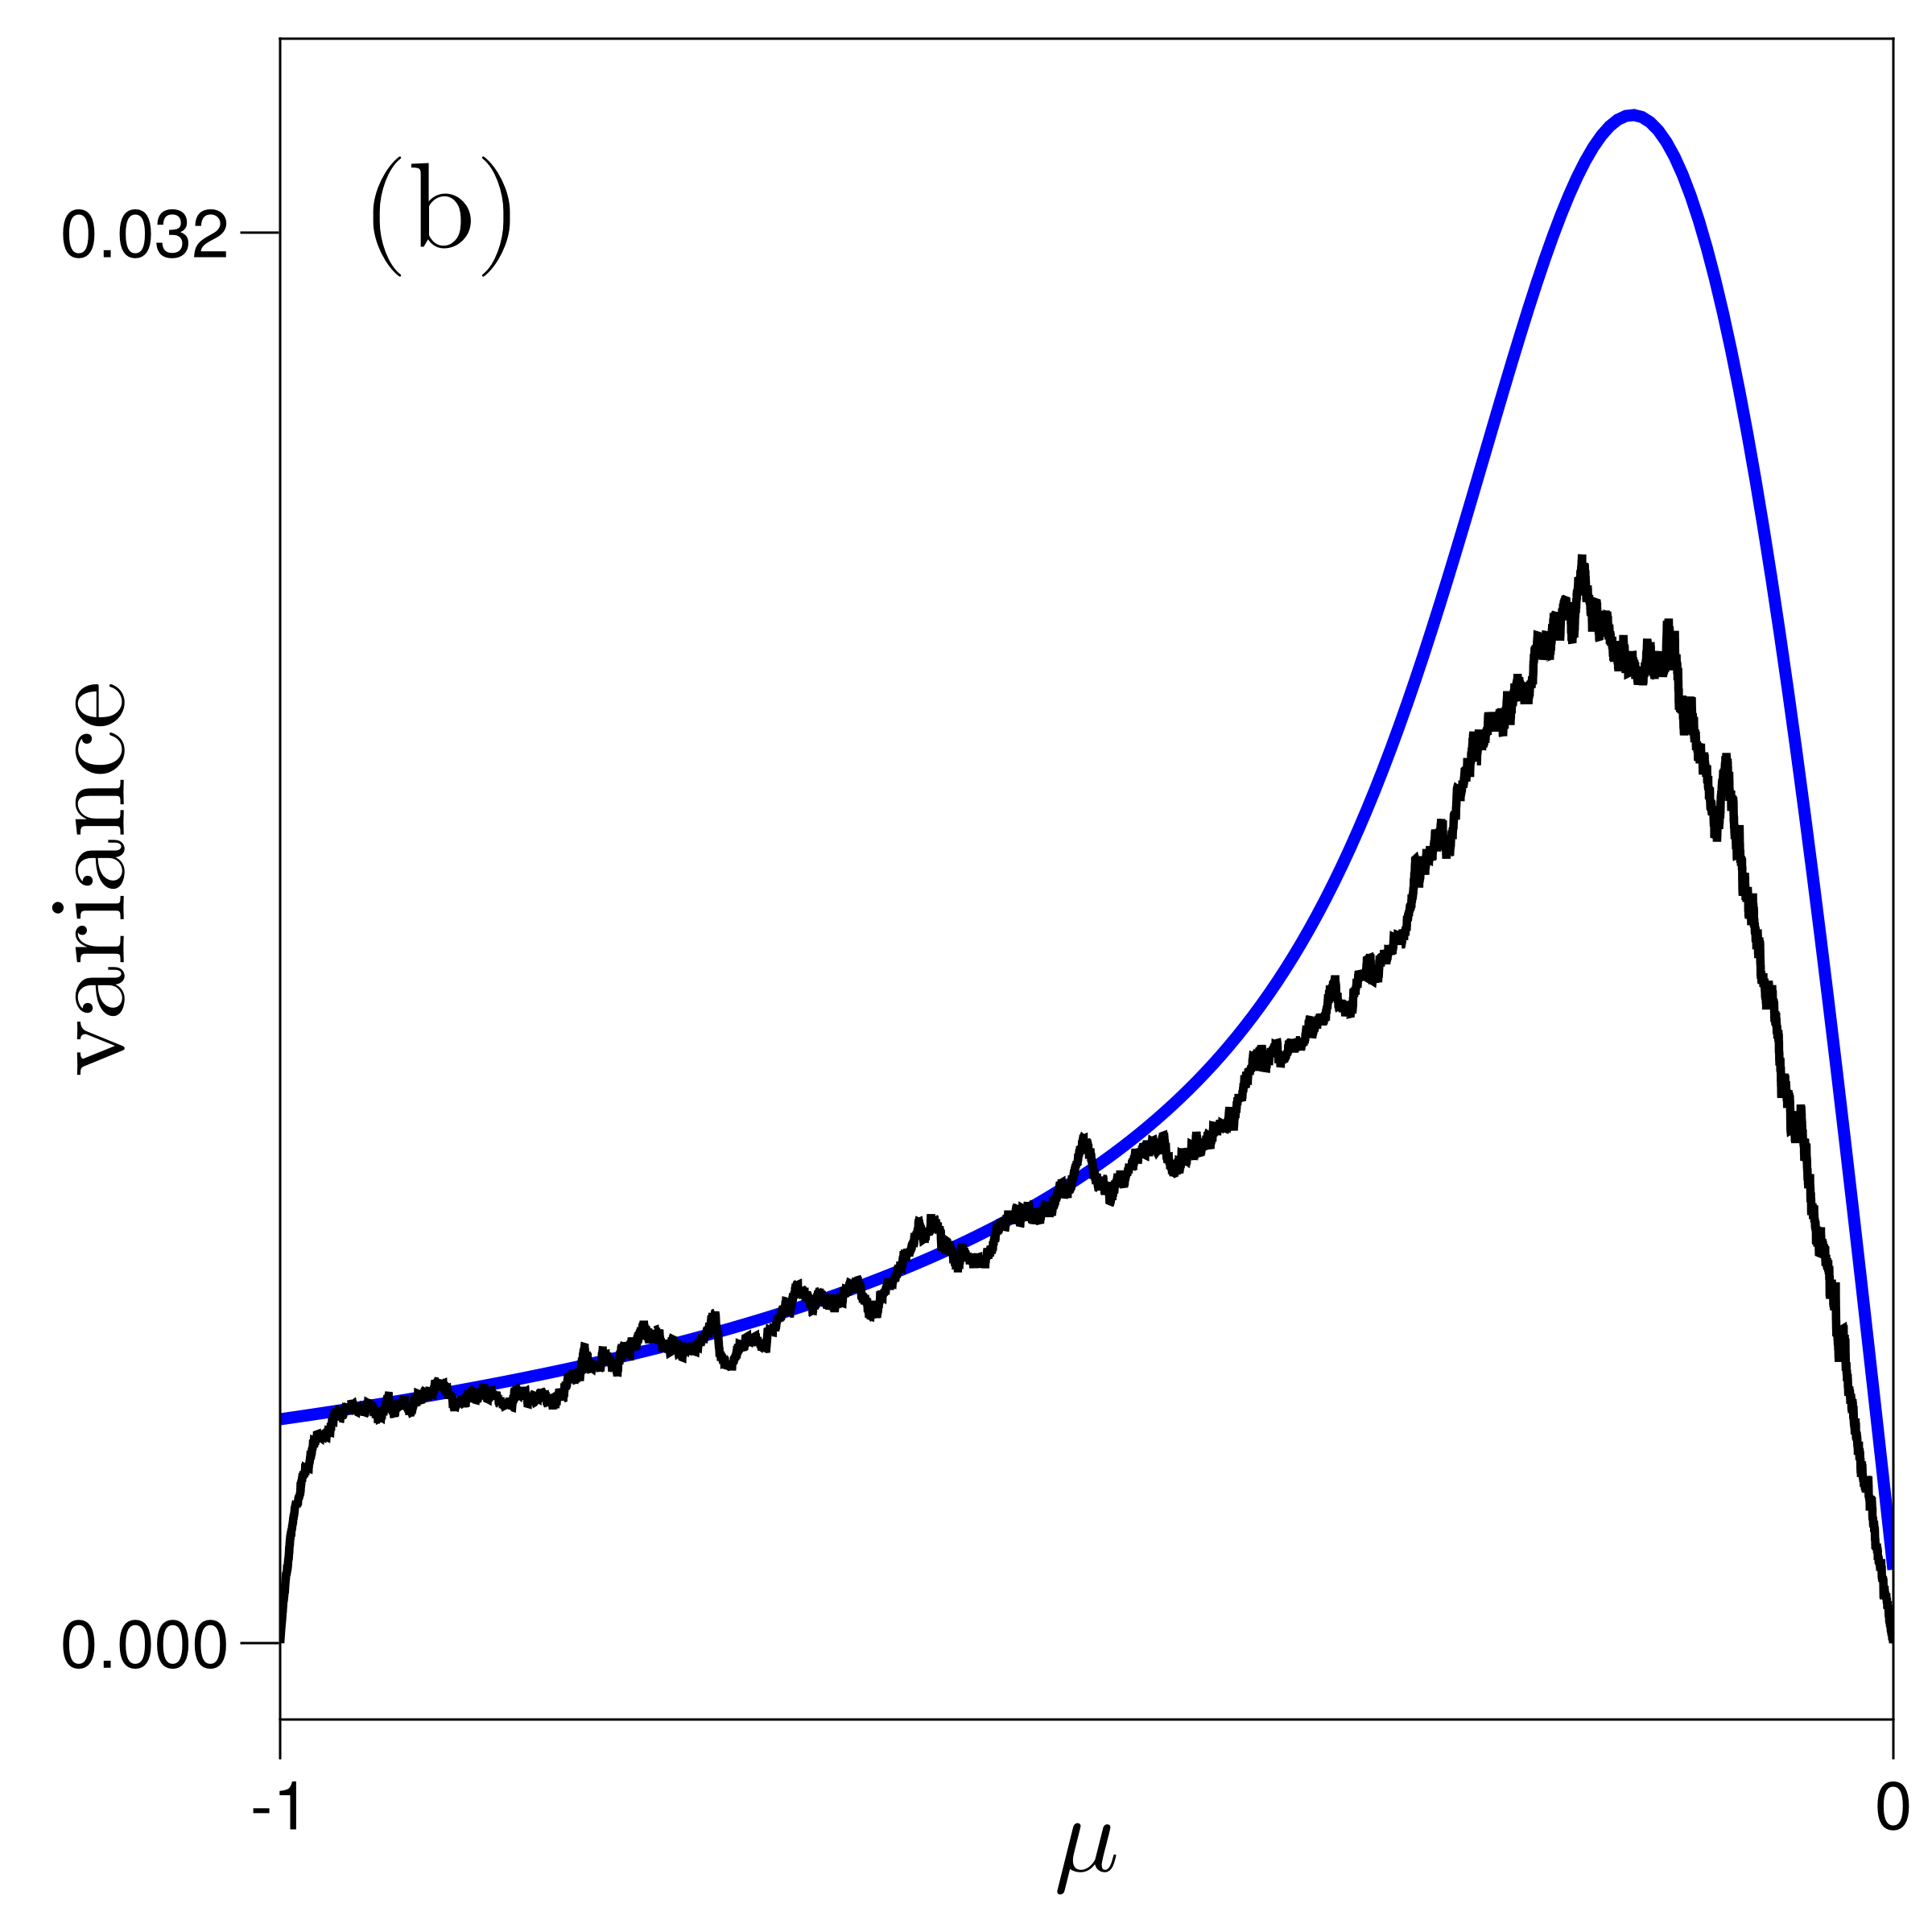
\includegraphics[keepaspectratio, width = \textwidth]{../figures/fig3.5.2.png}
        \label{fig3.5.2}
    \end{subfigure}
    \hfill
    \begin{subfigure}[b]{0.3\textwidth}
        \centering 
        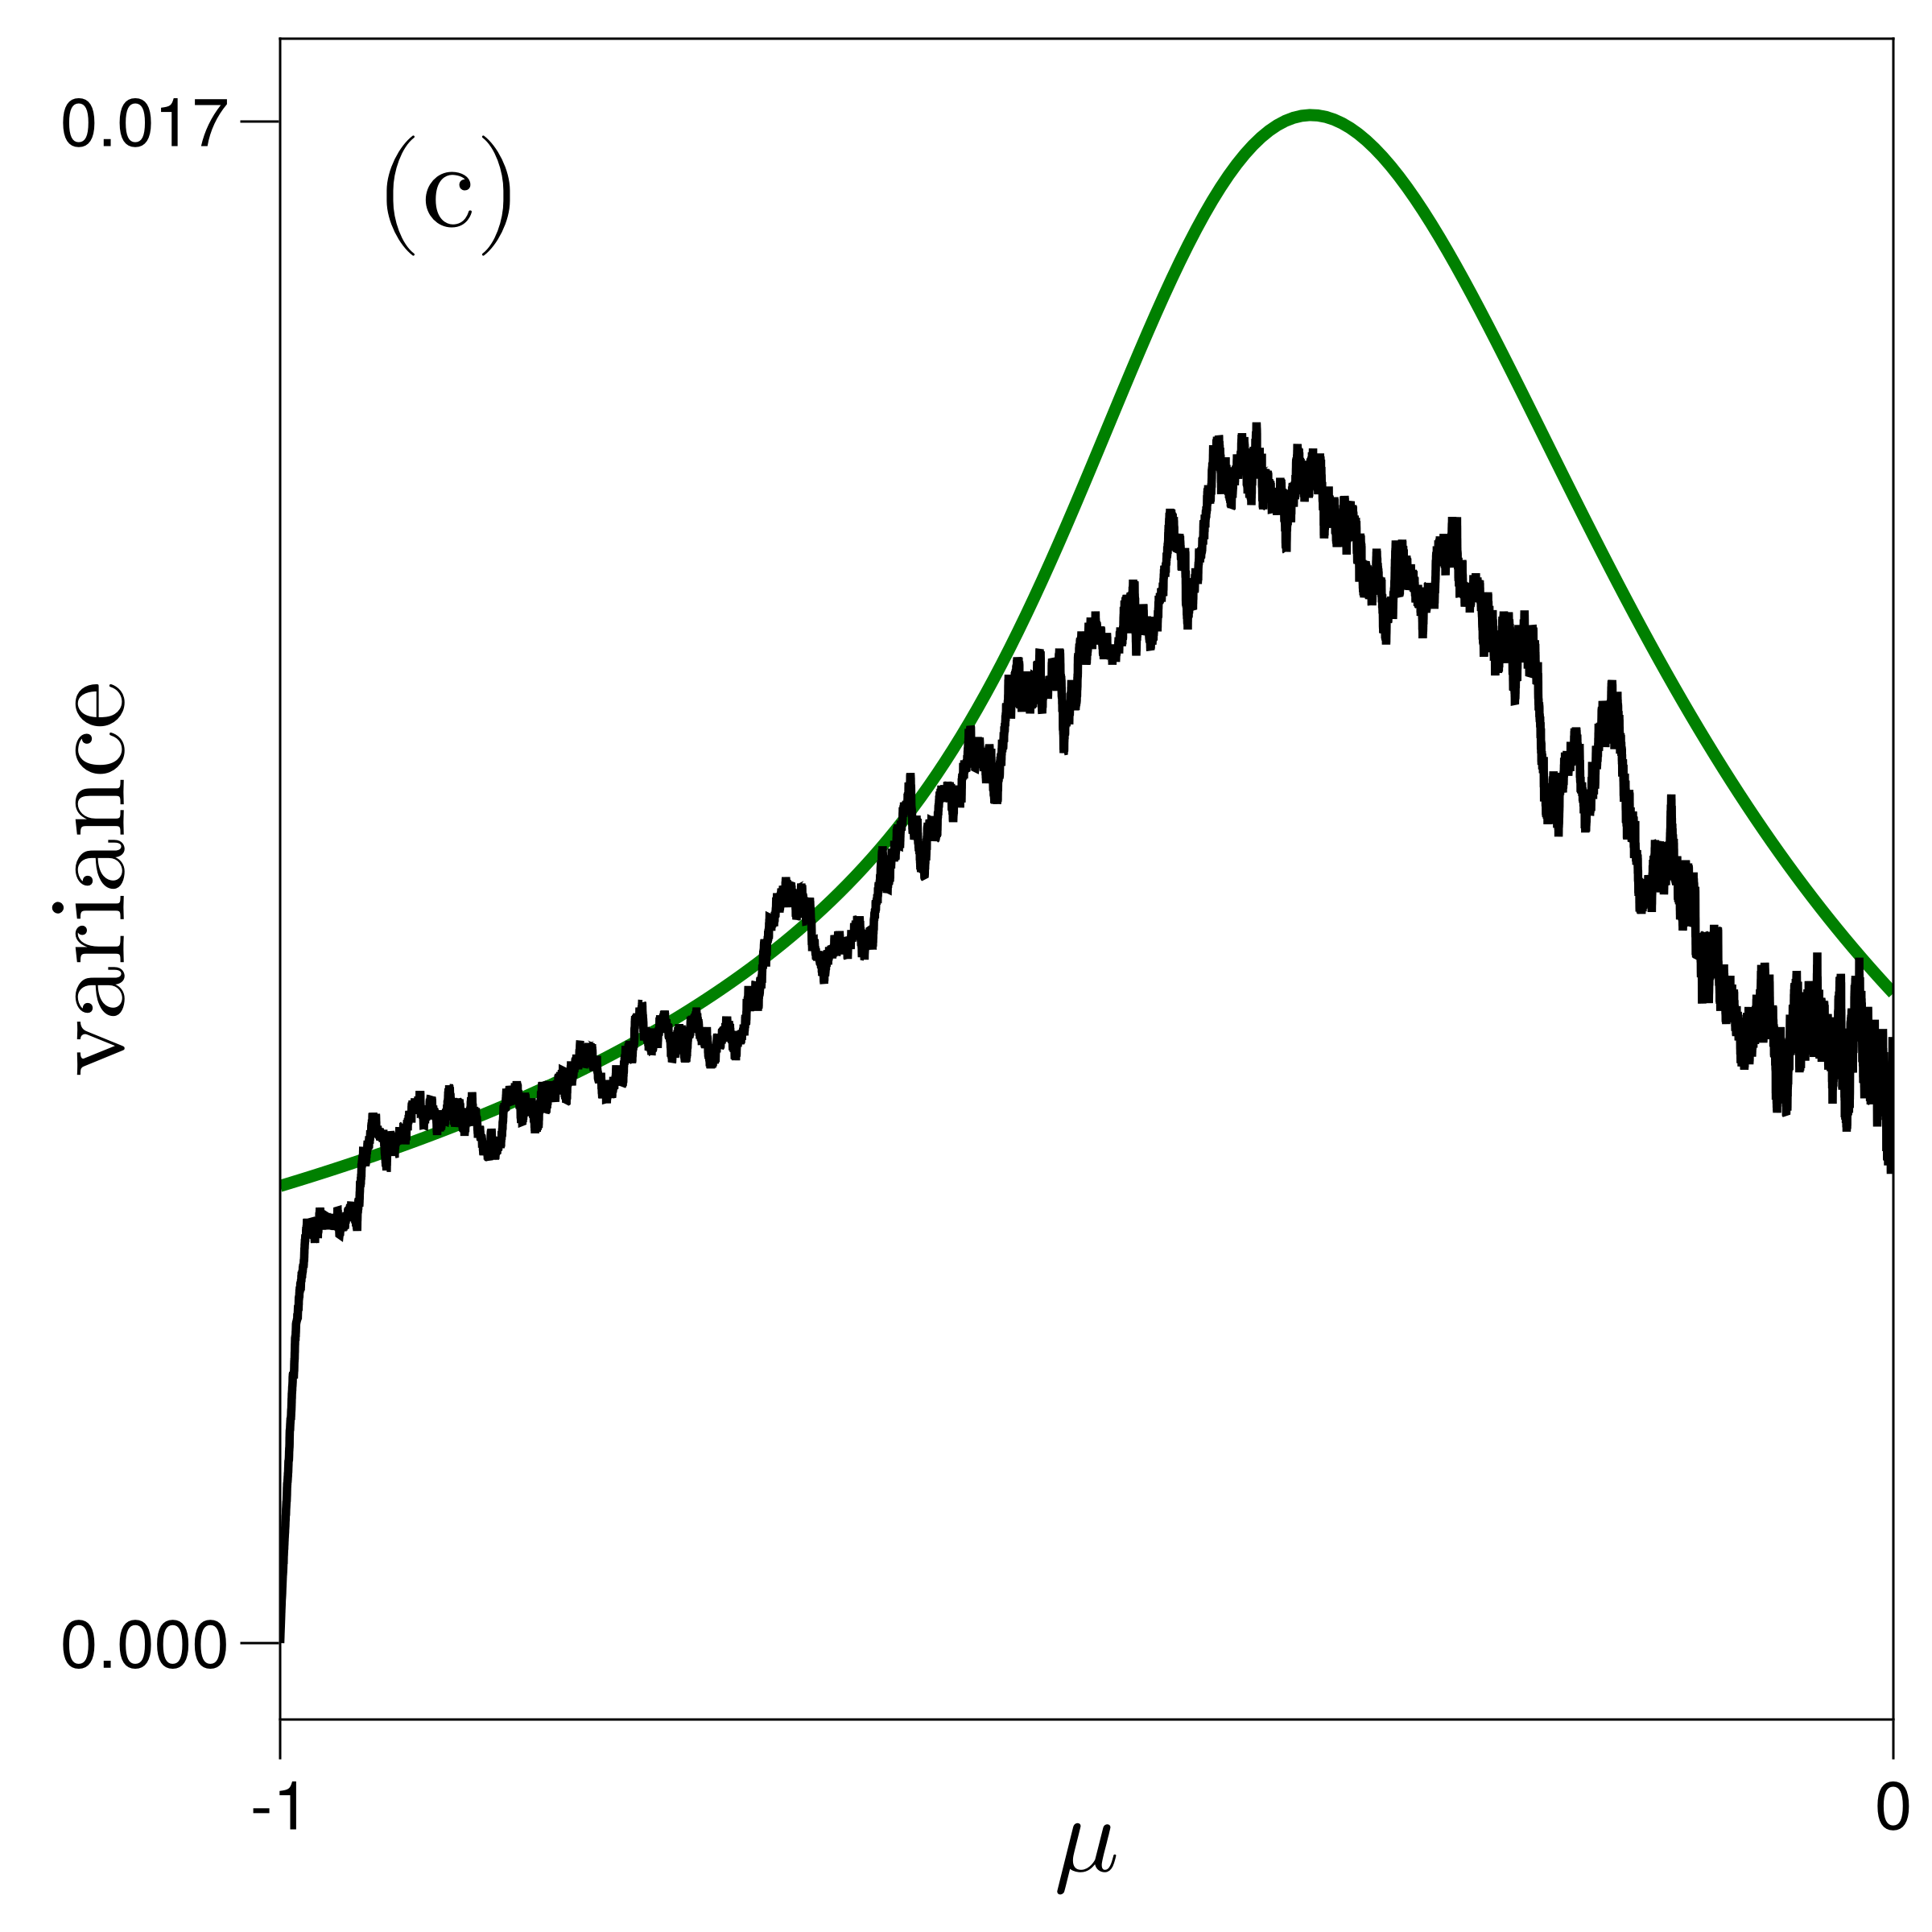
\includegraphics[keepaspectratio, width = \textwidth]{../figures/fig3.5.3.png}
        \label{fig3.5.3}
    \end{subfigure}
    \caption{Comparison between the analytical variance of the stationary Fokker-Planck distribution of the saddle-node (a), pitchfork (b) and transcritical (c) normal forms (colored lines) against the numerical variance of an ensemble of $1000$ sample paths (black lines) for the same cases (noise level $\sigma = 0.1$).}
    \label{fig3.5}
\end{figure}
The second most evident observation concerns the discrepancies between the analytical and numerical variance near the local maxima. In all three cases in fact we observe that the two curves agree when the parameter's values are far away from the deterministic critical transition however they largely differ as the parameter value gets closer to the local maxima for the analytical variance.
We can ascribe such discrepancy to (a) the choice that we made in counting the ensemble's sample paths as escaped (i.e. in counting N-tipping events) the exact moment they cross the unstable branch of the critical manifold and (b) the fact that while the analytical variance of the FPE is derived in the singular limit $\varepsilon=0$ (due to the stationarity assumption) the ensemble variance is computed within the fast-slow framework.
The first condition (a) actually imposes absorbing boundary conditions to our FPE which quite substantially differ from the reflecting boundary conditions used in the analytical derivation especially when boundary and noise effects become dominant (i.e. close to the deterministic critical transition as the basin of attraction shrinks further and further in size).
The second condition (b) emphasizes as the solution of the reduced equation in the singular limit is only an approximation of the full fast-slow dynamics.
This argument is validated further by observing how the discrepancy between the analytical and numerical variance for the saddle-node bifurcation is significantly less than those for the remaining two normal forms; based on this observation we expect fewer trajectories to escape the stable equilibrium for the saddle-node normal form and this is exactly what we observe in the ensemble simulations as depicted below in Figure \ref{fig3.6}.
\begin{figure}[H]
    \centering 
    \begin{subfigure}[b]{0.95\textwidth}
        \centering 
        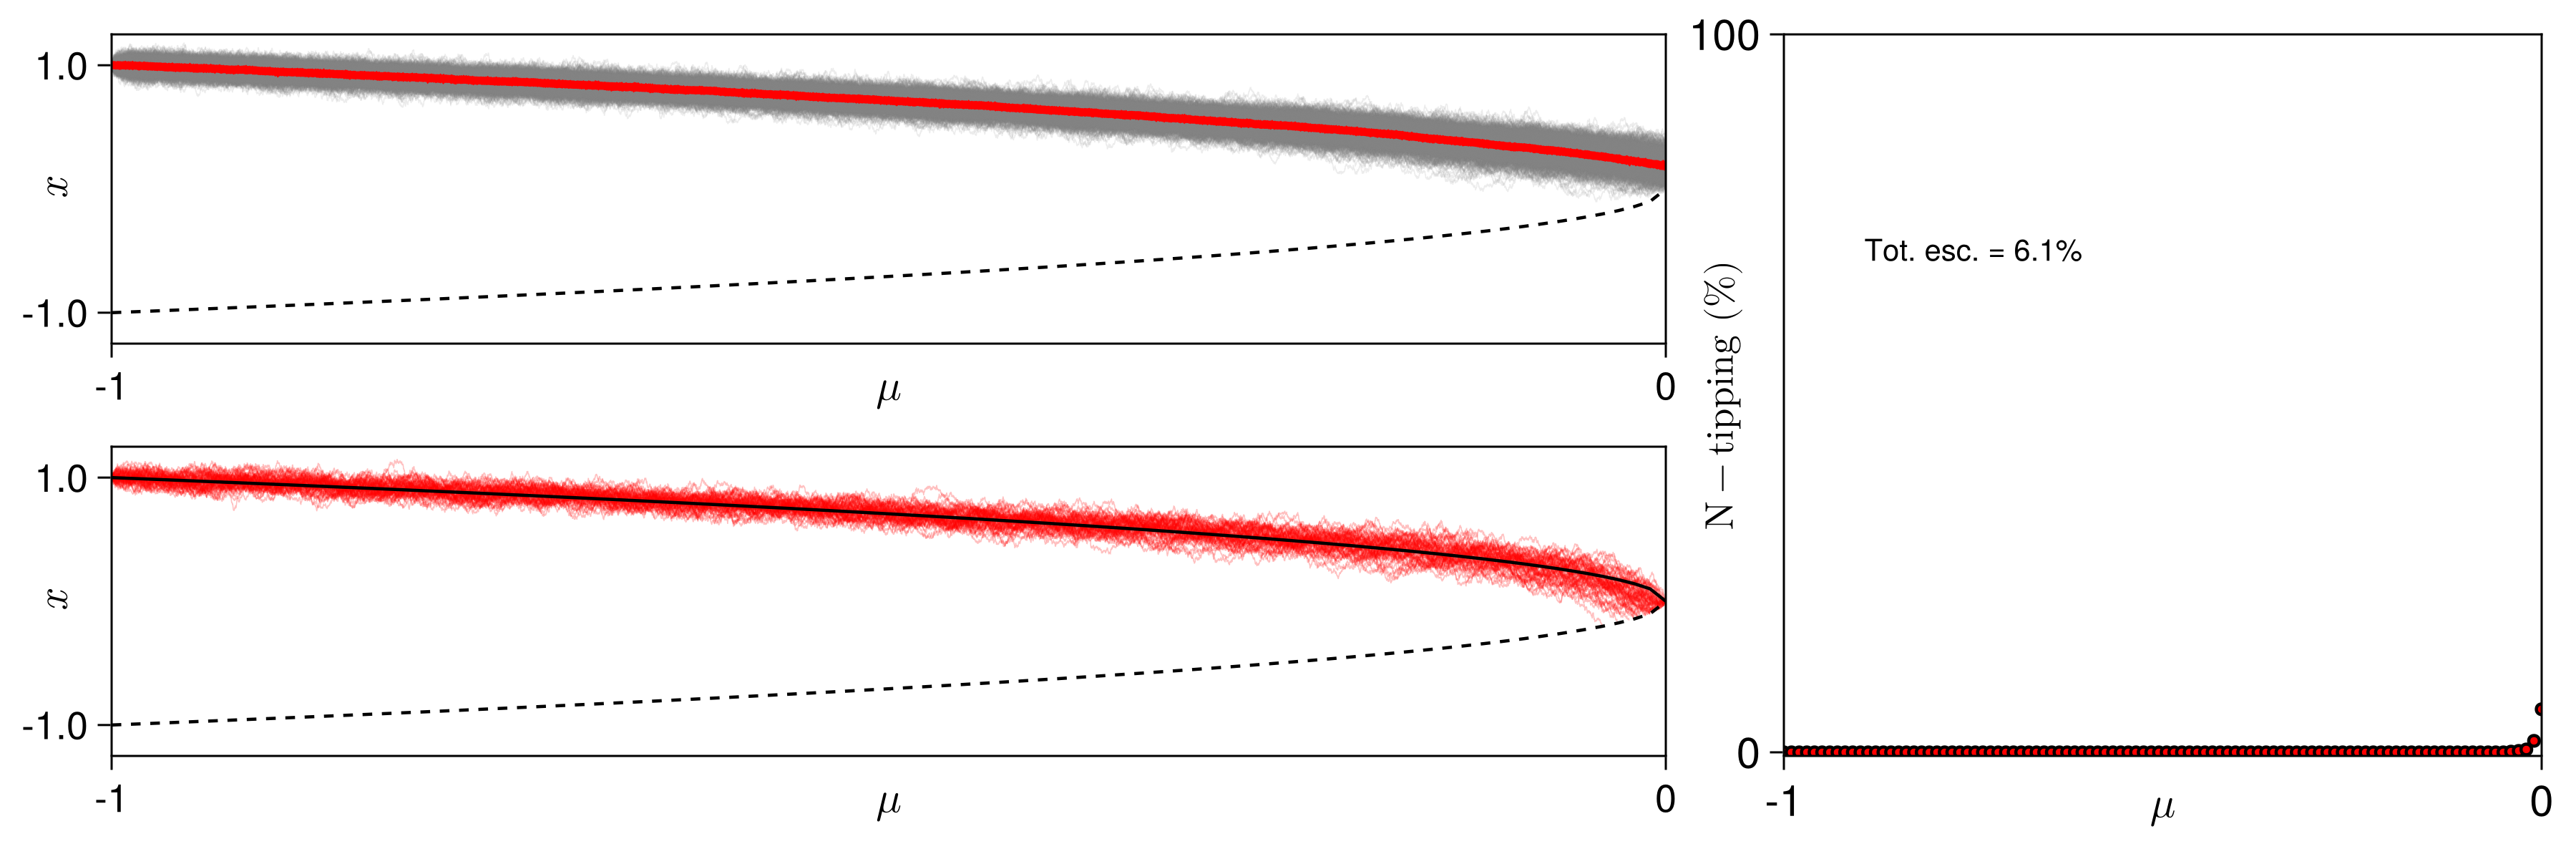
\includegraphics[keepaspectratio, width = \linewidth]{../figures/fig3.6.1.png}
        \label{fig3.6.1}
    \end{subfigure}
    \hfill 
    \begin{subfigure}[b]{0.95\textwidth}
        \centering 
        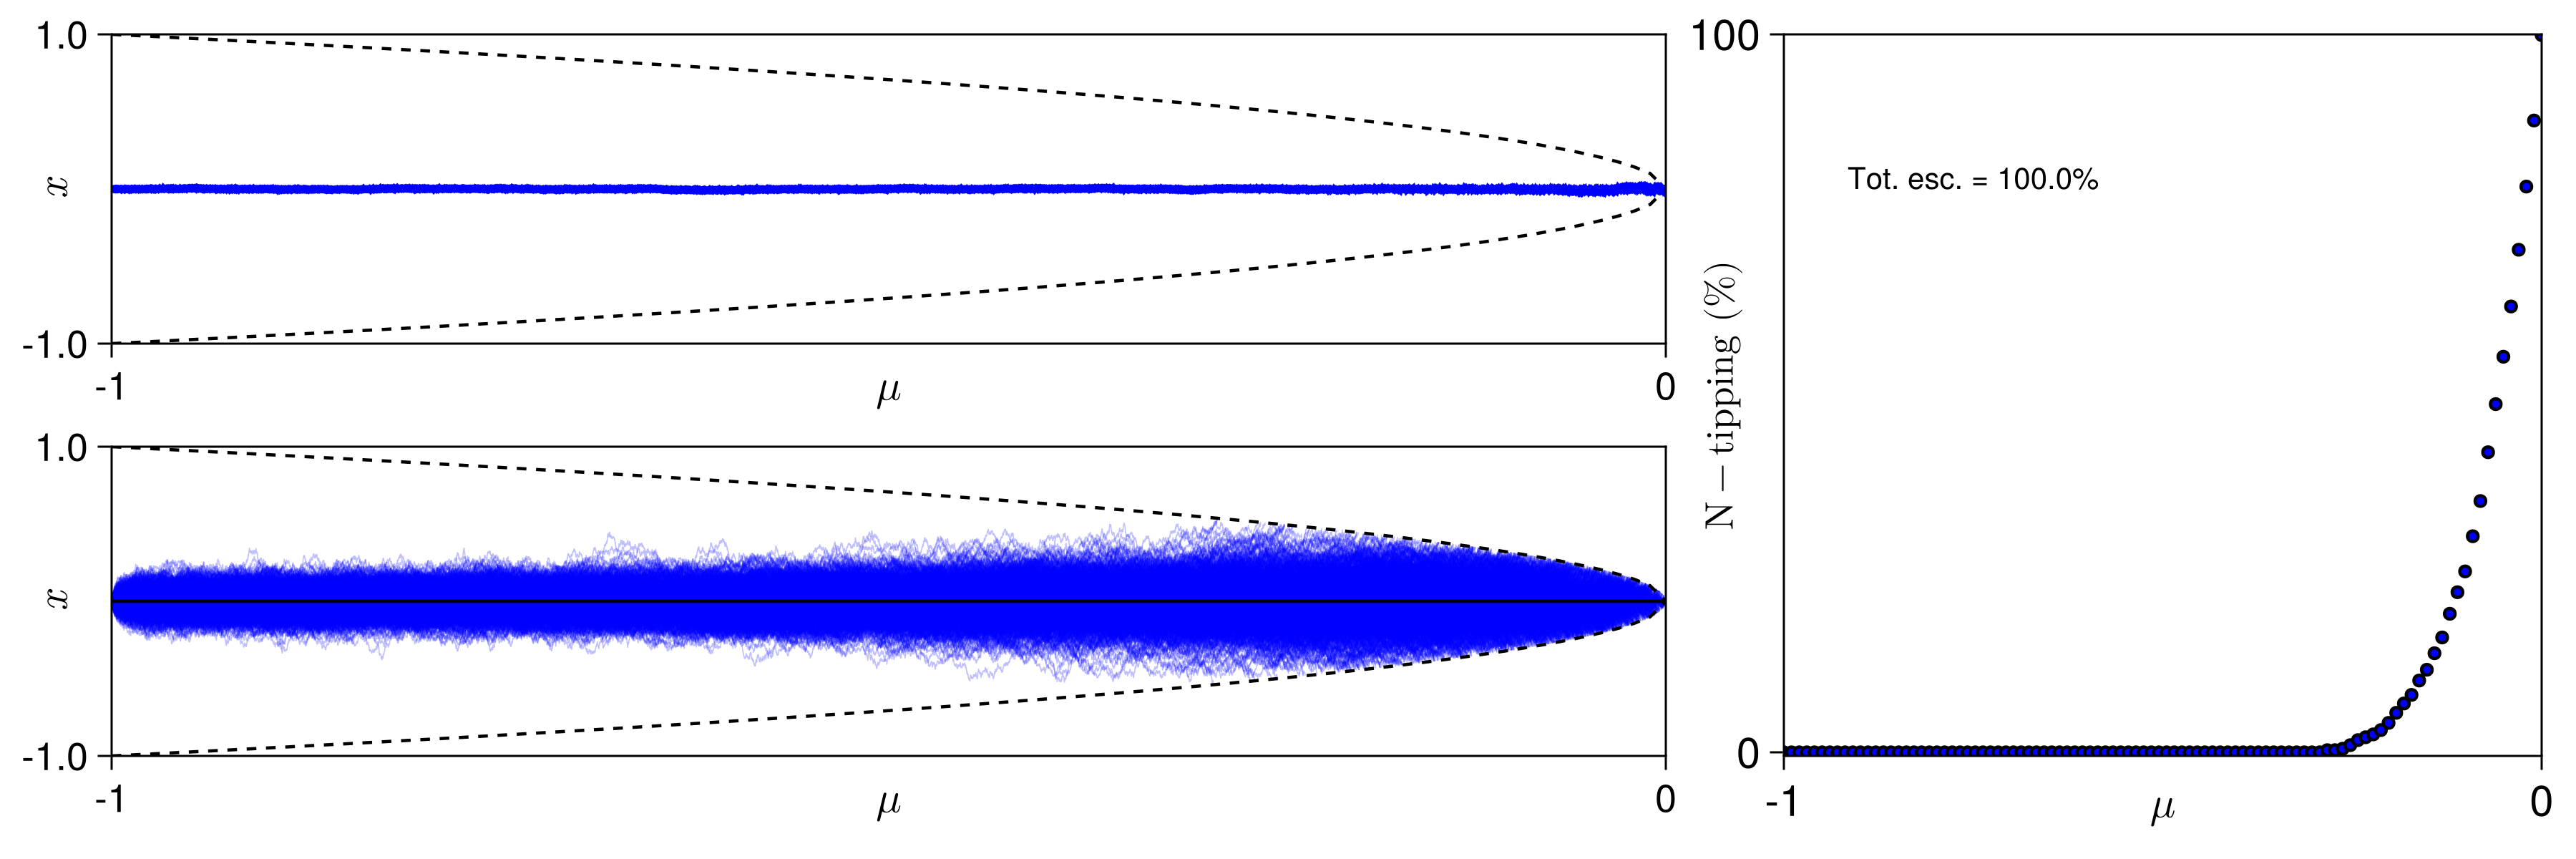
\includegraphics[keepaspectratio, width = \linewidth]{../figures/fig3.6.2.png}
        \label{fig3.6.2}
    \end{subfigure}
    \hfill
    \begin{subfigure}[b]{0.95\textwidth}
        \centering 
        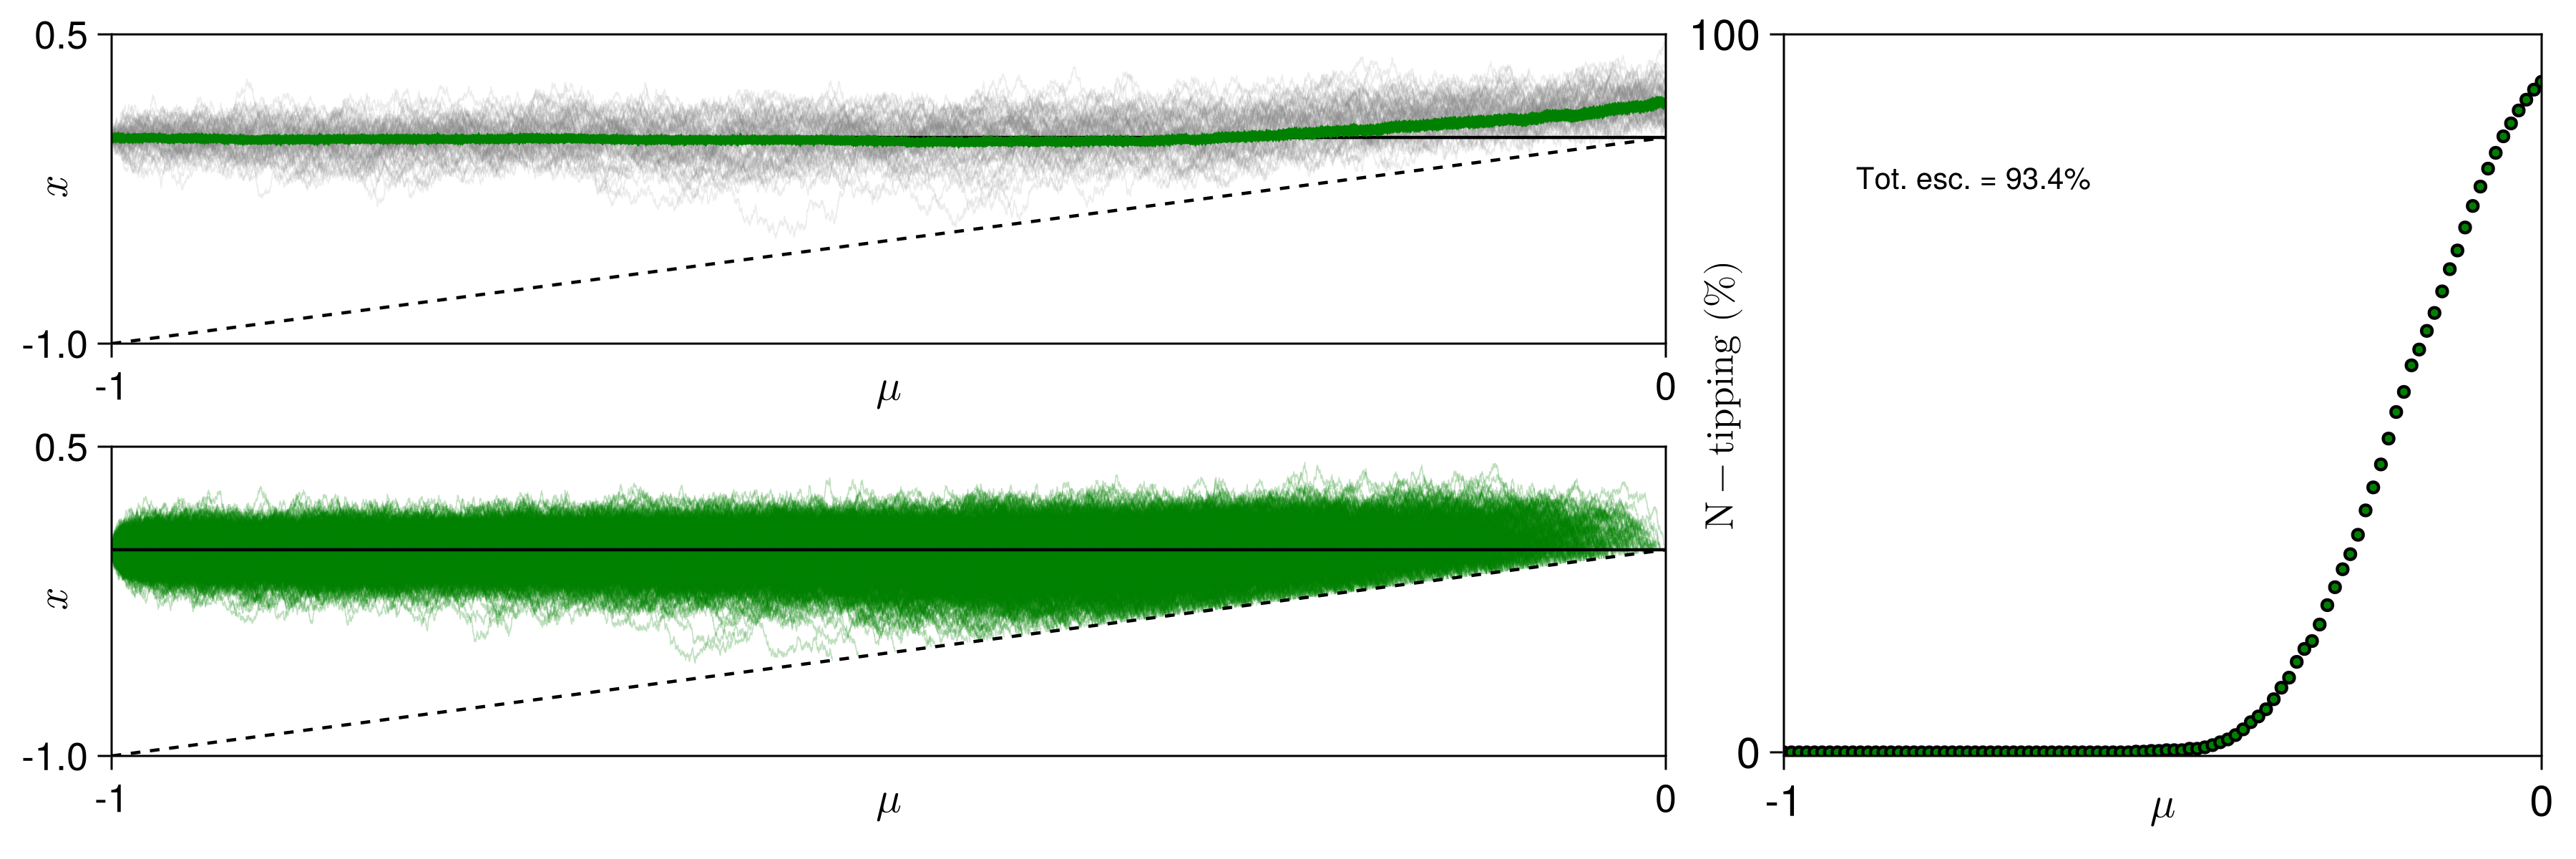
\includegraphics[keepaspectratio, width = \linewidth]{../figures/fig3.6.3.png}
        \label{fig3.6.3}
    \end{subfigure}
    \caption{Ensemble sample paths of saddle-node (top), pitchfork (middle) and transcritical (bottom) normal forms showing the trajectories that stayed bounded on the stable branch of the critical manifold (top panels: gray lines indicate the ensembles trajectories and the colored lines show the ensemble mean) and those that escaped due to N-tipping (bottom panels). 
    On the left of each plot a percentage of the number of escaped trajectories as $\mu$ vaires is shown.}
    \label{fig3.6}
\end{figure}
\begin{example}[label=ex3.4]{}{}
Consider the case of a transcritical normal form with multiplicative noise
\begin{equation*}
         dx = (\mu x - x^{2} + \frac{1}{2}\sigma^{2}x)\,dt + \sigma x\,dW\,,
\end{equation*}
as presented in \cite{Kuehn11}. 
We write the associated FPE which, in the singular limit, it reads
\begin{equation*}
          0 = -\frac{d}{dx}((yx - x^{2} + \frac{1}{2}\sigma x)p_{s}(x; y)) + \frac{d^{2}}{dx^{2}}(\frac{1}{2}\sigma^{2}x^{2}\,p_{s}(x; y))\,.
\end{equation*}
One normalizable solution of the above stationary FPE is
\begin{equation*}
          p_{s}(x) = \frac{1}{N_{\mu}}\,x^{\frac{2\mu}{\sigma^{2}}-1}\,e^{-\frac{2x}{\sigma^{2}}}\,,\quad N_{\mu}=\int_{0}^{+\infty} x^{\frac{2\mu}{\sigma^{2}}-1}\,e^{-\frac{2x}{\sigma^{2}}}\,dx = \bigg(\frac{\sigma^{2}}{2}\bigg)^{\frac{2\mu}{\sigma^{2}}}\,\Gamma\bigg(\frac{2\mu}{\sigma^{2}}\bigg)\,.
\end{equation*}
We recall the definition of the $\Gamma-$probability density function
\begin{equation}\label{eq3.15}
     f_{\alpha,\beta}(x):=\frac{1}{\Gamma(\alpha)}x^{\alpha-1}e^{-\beta x}\beta^{\alpha}
\end{equation}
where $\Gamma(z):=\int_{0}^{\infty}y^{z-1}e^{-y}dy$ is the Euler's Gamma function for $z\in \mathbb{C}$ while $\alpha,\beta\in \mathbb{R}$ parametrise the distribution.
The first central moments of \eqref{eq3.14} are well known, in particular
\begin{equation}\label{eq3.16}
     \mathbb{E}_{f}(x;\alpha,\beta) = \frac{\alpha}{\beta}\,,\quad \text{Var}_{f}(x;\alpha,\beta)=\frac{\alpha}{\beta^{2}}\,.
\end{equation}
With a simple change of variables we immediately verify that the normalised solution of the FPE of the transcritical stochastic process with linear, multiplicative noise, is equivalent to \eqref{eq3.14}
\begin{equation*}
    \alpha = \frac{2\mu}{\sigma^{2}}\,,\quad \beta=-\frac{2}{\sigma^{2}}\,. 
\end{equation*}
Putting the above into \eqref{eq3.16} yields
\begin{equation*}
     \mathbb{E}_{p_{s}}(x;\mu)=\mu\,,\quad \text{Var}_{p_{s}}(x;\mu)=\frac{\sigma^{2}}{2}\mu\,.
\end{equation*}
What is left to verify is that under the above change of variables the normalisation constant $N_{\mu}$ coincides with that of the $\Gamma-$distribution.
We write
\begin{equation*}
     N_{\mu}=\int_{0}^{\infty}x^{\frac{2\mu}{\sigma^{2}}-1}e^{-\frac{2x}{\sigma^{2}}}dx\,,
\end{equation*}
and perform a $u-$substitution $x=\frac{\sigma^{2}}{2}u\,\rightarrow dx=\frac{\sigma^{2}}{2}du$ to get
\begin{equation*}
     N_{\mu}=\int_{0}^{\infty}\frac{\sigma^{2}}{2}\bigg(\frac{u\sigma^{2}}{2}\bigg)^{\frac{2\mu}{\sigma^{2}}-1}e^{-u}du\,,
\end{equation*}
which can be integrated by parts yielding
\begin{equation*}
        N_{\mu}=\bigg(\frac{\sigma^{2}}{2}\bigg)^{\frac{2\mu}{\sigma^{2}}-1}\bigg(\frac{\sigma^{2}}{2}\bigg)\int_{0}^{\infty}u^{\frac{2\mu}{\sigma^{2}}-1}e^{-u}du=\bigg(\frac{\sigma^{2}}{2}\bigg)^{\alpha}\int_{0}^{\infty}u^{\alpha}e^{-u}du = \bigg(\frac{\sigma^{2}}{2}\bigg)^{\alpha}\Gamma(\alpha)\,.
\end{equation*}
\end{example}
\begin{example_continued}
\begin{figure}[H]
        \begin{subfigure}[b]{0.95\textwidth}
                \centering 
                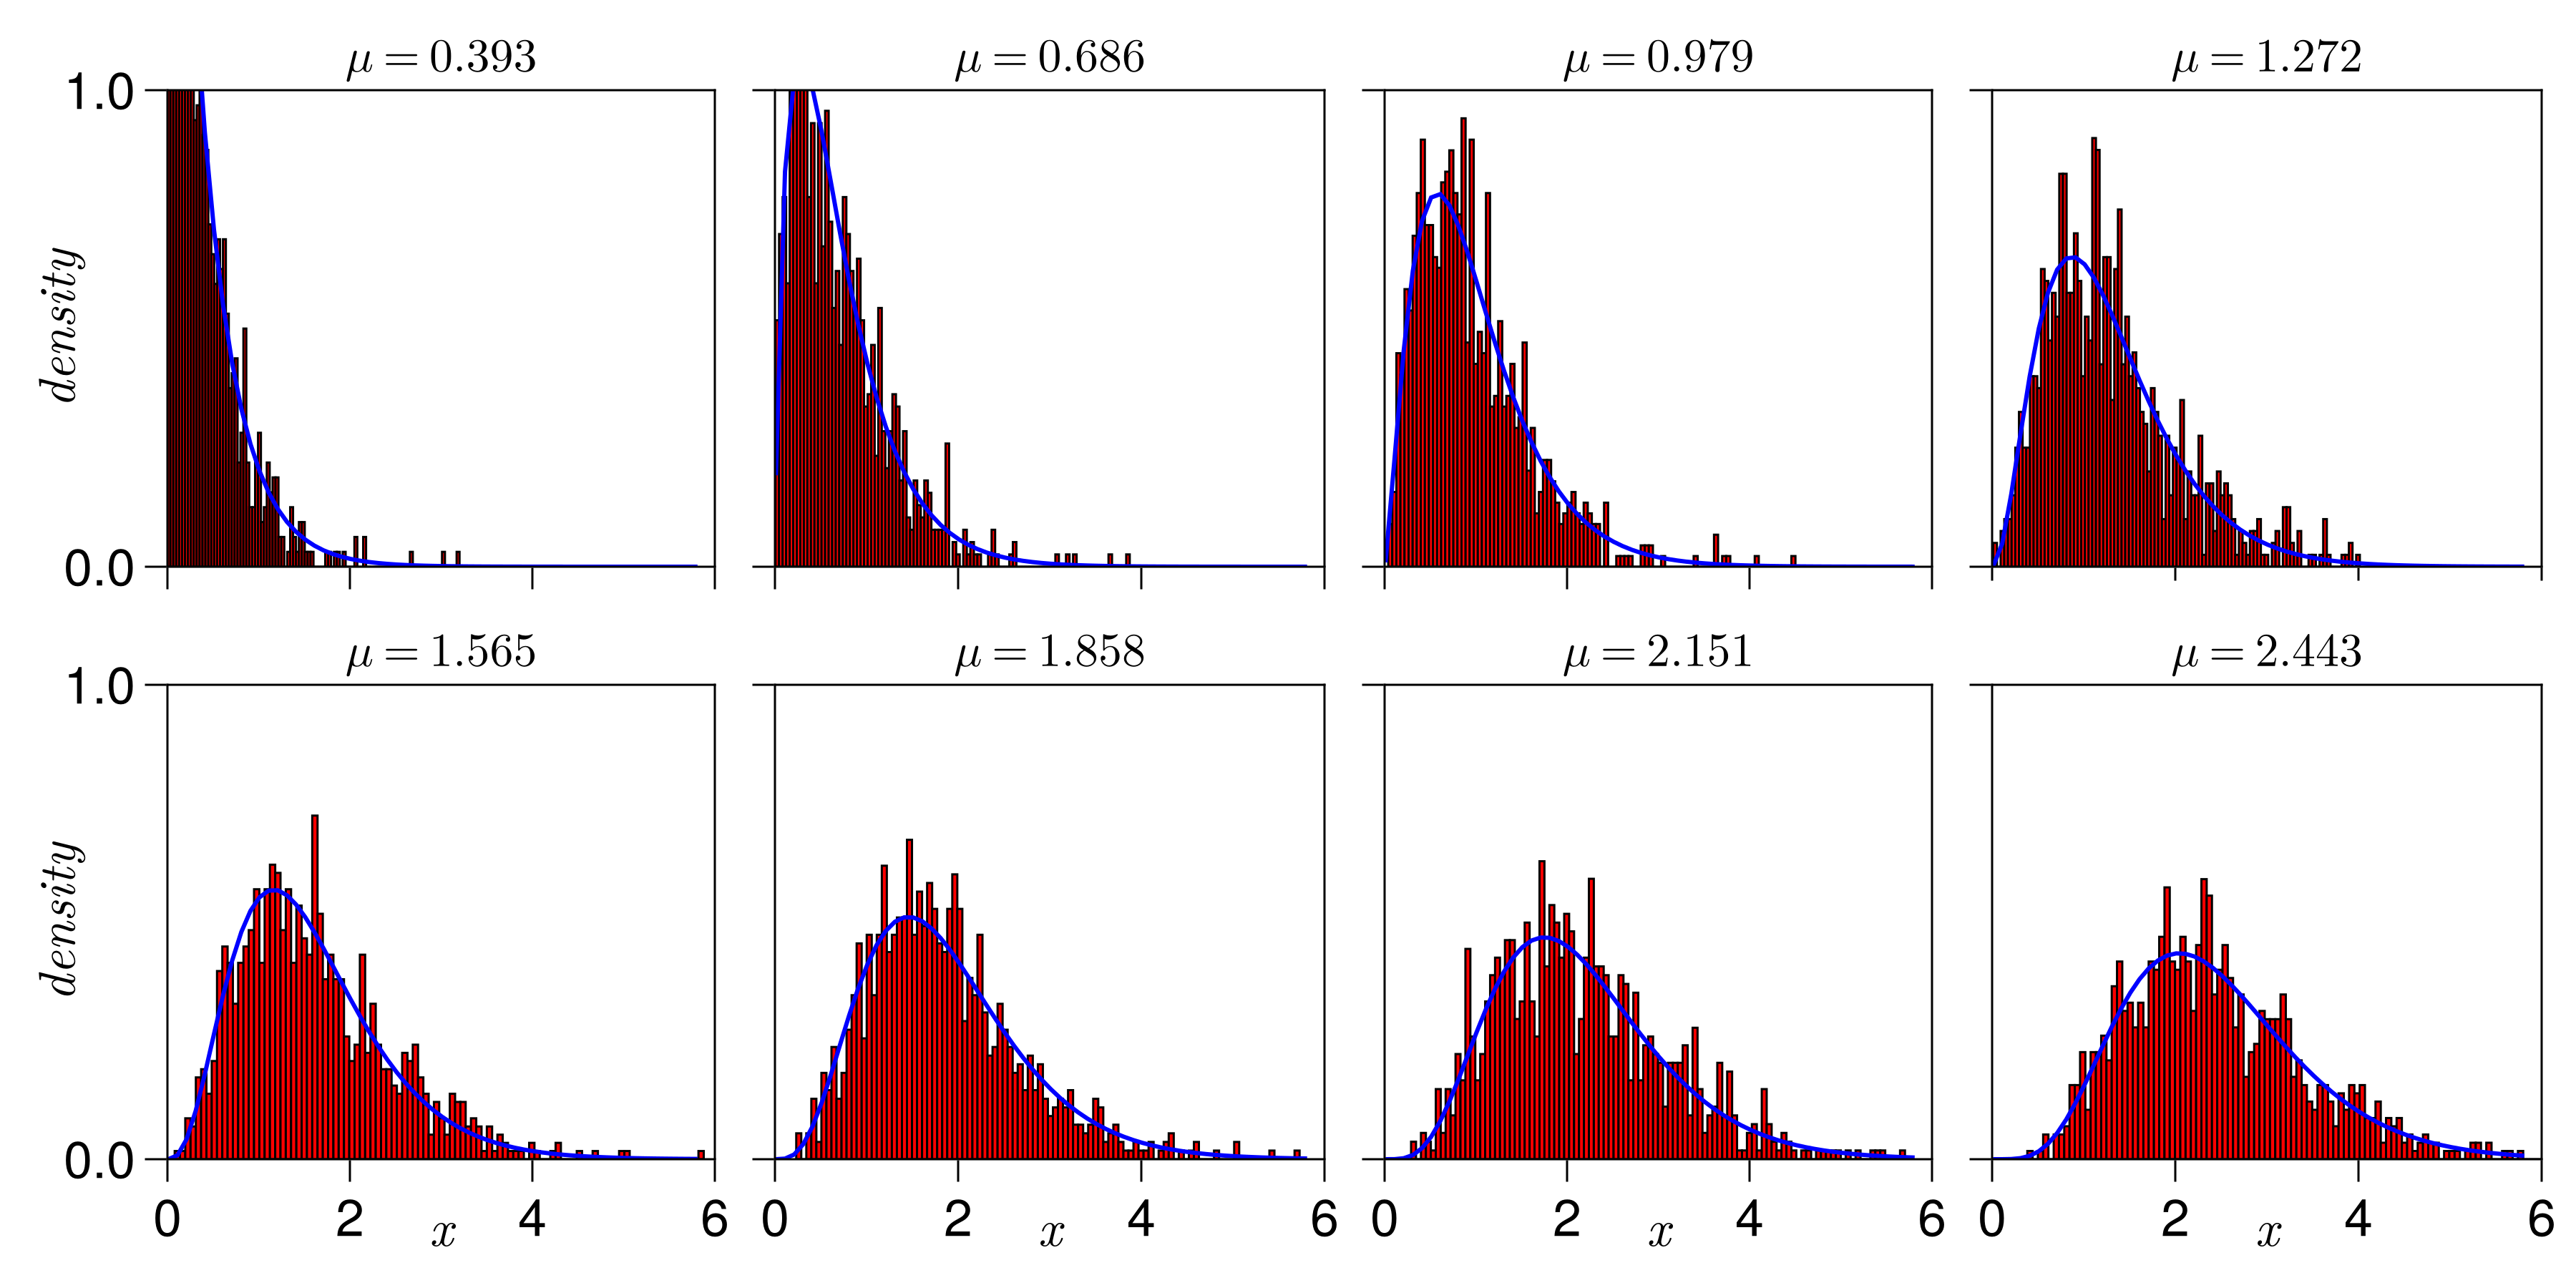
\includegraphics[keepaspectratio, width = \linewidth]{../figures/fig3.7.1.png}
                \label{fig3.7.1}
                \caption{}
        \end{subfigure}
        \newpage
        \begin{subfigure}[b]{0.95\textwidth}
                \centering 
                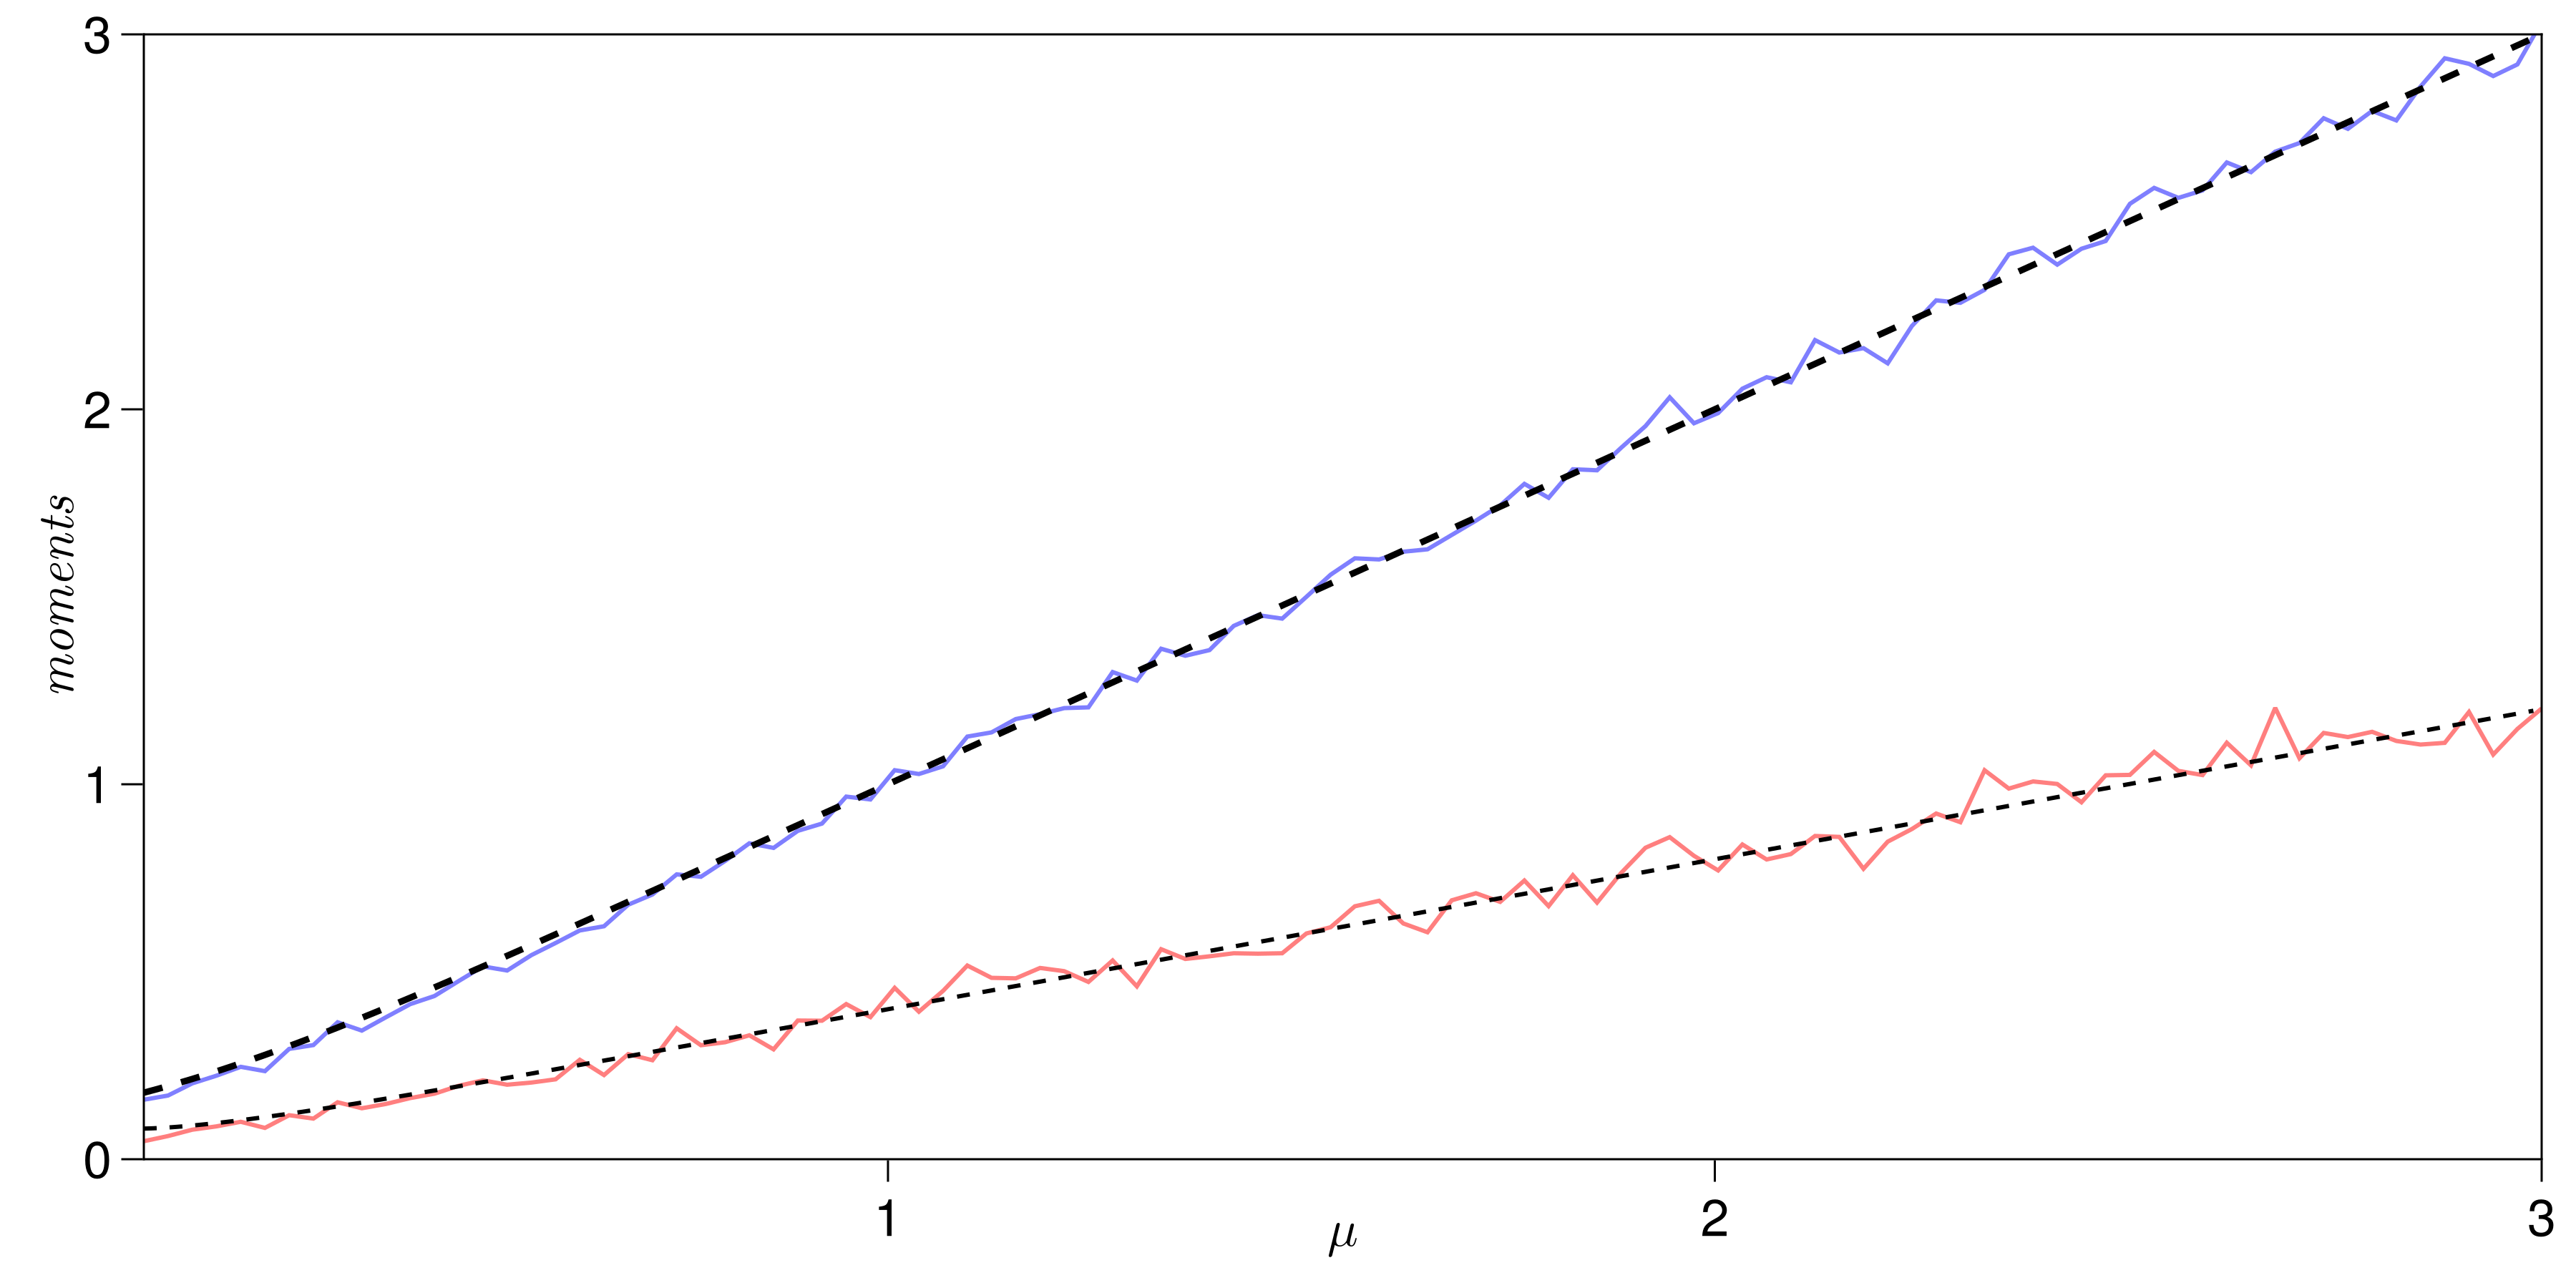
\includegraphics[keepaspectratio, width = \linewidth]{../figures/fig3.7.2.png}
                \label{fig3.7.2}
                \caption{}
        \end{subfigure}
         \caption{(a) Snapshots of the stationary Fokker-Plank distribution $p_{s}(x)$ (solid blue lines) for the transcritical normal form with multiplicative noise scaled by $\sigma = \sqrt{0.8}$ at different values of the parameter overlayed with histograms (red bars) associated to an ensemble simulation of $1000$ sample paths. (b) Comparison between the analytical parameter variation of the mean and variance of the stationary FPE (dashed black lines) with the sample estimates from the ensemble trajectories (ensemble average in blue while variance is in red).}
         \label{fig3.7}
\end{figure}
\end{example_continued}
\subsection{High-dimensional systems}\label{subsec3.2}
The construction of a dynamical model that exhibits tipping points driven by different phenomena has so far relied on a number of assumptions that have been subsequently relaxed in order to achieve a more flexible and realistic mathematical description of observed critical events. 
Throughout the previous analysis we have however restricted ourselves in considering a finite number of observables whose time-evolution, if taken to be a model of real phenomena defined on a spatio-temporal domain, represent the dynamics of spatially-aggregate measures.
In other words we have so far only consider observables that are instrincly defined over a spatial domain whose change with time happens uniformly throughout space. This simplification is powerful, as it allowed the derivation of robust mathematical frameworks in e.g. \cite{Kuehn11} and \cite{Ashwin12} for the analysis of tipping events and their precursors however it also implies the discard of any potential instantaneous change in the spatial distribution of those state variables.
Indeed ignoring how obervables change in space and only considering the time-evolution of their properties automatically restrict the analysis of either events that are not defined on a spatial domain or spatially heterogeneous models that we can only measure in an aggregate sense (i.e. by considering spatial means of the observables).
In both instances, relying on such simplification heavily implies the loss of meaningfull information and methods of mathematical analysis thus preventing the detection of precursors s.a. self-organising pattern-formation.
As such this last strong assumption of spatial homogeneity will be dropped as we will now consider observables $x\mapsto u(x)$, $x\in \Omega\subseteq\mathbb{R}^{d}$ ($d=1,2,3$) as (scalar) functions varying in both space and time.
These functions $u(x,t)\in V\times \mathbb{R}^{+}$ can be thought as solutions of space-time partial differential equations (PDEs) on a functional space $V$ which is infinite dimensional.
We will thus refer to these spatio-temporal dynamical systems, whose phase space coincides with $V$, as high-dimensional as opposed to the low-dimensional case insofar treated for a set of finite observables $x\in \mathbb{R}^{n}$ with $n\ll\infty$.
\subsubsection{Intrinsic discrete phenomena}\label{subsubsec3.2.1}
As an intermediate step between low and high-dimensional problems, lattice dynamical systems (LDSs) have been investigated in the context of EWS detection. These are (large) systems of coupled ODEs organised on a $d-$dimensional regular lattice; each of such ODEs models the dynamics of the same observable $u$ at a given lattice site (node).
These systems are therefore intrisicly discrete in space while still retaining spatial heterogeneity via the coupling of the system.
As such one can use the temporal indicators derived above for low-dimensional systems while enriching the analysis by considering spatial statistics at each timestep of observation.
One specific model of interest has captived the efforts of recent works towards the construction of a robust theory of spatio-temporal EWS and that is the reaction-diffusion problem.
Given a $2-$dimensional rectangular lattice of $n\times m$ nodes, a generic reaction-diffusion problem perturbed by additive noise can be written, in cartesian coordinates, as
\begin{equation}\label{eq3.17}
     du_{j,k} = (D_{j,k}\,\phi(u_{j,k}, u_{j\pm1,k}, u_{j,k\pm1}) + R_{j,k}\,\psi(u_{j,k}))\,dt + \sigma\,dW_{j,k}\,,
\end{equation}
where $\phi$ represents the nearest-neighbour coupling modelling the diffusion component while $\psi$ is responsible for the reaction of $u$ at lattice site $(j,k)$.
A trivial transfortmation $\ell=n(k-1)+(j+1)$ allows us to recast \eqref{eq3.16} in linear coordinates
\begin{equation}\label{eq3.18}
     du_{\ell} = (D_{\ell}\,\phi(u_{\ell}, u_{\ell\pm1}, u_{\ell\pm n}) + R_{\ell}\,\psi(u_{\ell}))\,dt + \sigma\,dW_{\ell}\,,
\end{equation}
which is more convenient for our analysis.
The inclusion of a slowly-varying parameter $\mu$ in \eqref{eq3.18} completes our intermediate model to a more general case
\begin{equation}\label{eq3.19}
   \begin{cases}
      du_{\ell} = (D_{\ell}(\mu)\,\phi(u_{\ell}, u_{\ell\pm1}, u_{\ell\pm n}; \mu) + R_{\ell}(\mu)\,\psi(u_{\ell}; \mu))\,dt + \sigma\,dW_{\ell} \,, \\
      d\mu = \varepsilon\,dt \,. 
   \end{cases}
\end{equation}
We end this section by noticing that $D$ and $R$ are (generally inhomogeneous) scalar fields assigning relative (local) magnitudes to the diffusion and reaction phenomena respectively and they are paramount in the analysis of the onset of instabilities in these problems as addressed in the following Section.
\subsubsection{Instabilities in reaction-diffusion problems}\label{subsubsec3.2.2}
Reaction-diffusion equations are of particular interest in mathematical modelling and analysis of differential equations because of how different instabilities of homogeneous stable states may cause very different asymptotic solutions: examples are travelling (stationary) waves, solitons, regular and irregular patterns.
In the context of this report and at large as the primary object of investigation of this research proposal going forward, the rise of spatial patterns from homogeneous solutions (Turing instabilities) will be considered as the tipping event of interest connecting two, very different steady-states of the system. 
We choose to target these particular events for two reasons:
\begin{itemize}
     \item to narrow the scope of an otherwise prohibitevely broad type of instabilities that can occur in high-dimensional systems;
     \item since they are observed to be peculiar to natural systems that exhibit transition from a \textit{healthy} state (e.g. homogeneous ventilation in the airways of a lung or locally homogeneous vegetation distribution in a florid ecosystem) to an \textit{unhealthy} one (onset of CVDs in a lung undergoing asthma and the rise of patches of turbidity prior desertification).
\end{itemize}
To illustrate simple techniques in detecting pattern formations in $2-$dimensional reaction-diffusion LDSs we consider first a model of vegetation turbidity analysed in \cite{Chen19}. From \eqref{eq3.19} we set
\begin{align}
        \phi(u_{\ell}, u_{\ell\pm1},u_{\ell\pm n}; \mu) =&\, u_{\ell+1}+ u_{\ell+1}+ u_{\ell-1} + u_{\ell+n} + u_{\ell-n}-4u_{\ell}\,, \nonumber \\
        \psi(u_{\ell}; \mu) =&\,r_{v}\,u_{\ell}\bigg(1-u_{\ell}\frac{r_{\ell}^{4}+E_{\ell}^{4}(\mu)}{r_{\ell}^{4}}\bigg)\,,\;E_{\ell}(\mu)=\mu\,\frac{h_{v}}{h_{v}+u_{\ell}} \,,\nonumber
\end{align}
with $r_{\ell}$ being sampled uniformly at random in $[0.6, 1.0]$ and independently for each lattice site while $r_{v} = 0.5$ and $h_{v} = 0.2$ are uniform throughout the domain. 
In the paper the authors aim at detecting the formation of irregular patterns by means of tracking the leading eigenvalue of the spatial covariance matrix $\Sigma\in \mathbb{R}^{N\times N}$ where $N:={n\cdot m}$ is the dimension of a single snapshot of the solution defined on a regular $n\times m$ lattice at each timestep.
The matrix is assembled considering $W$ consecutive snapshots collected in $\boldsymbol{\mathcal{X}}\in \mathbb{R}^{N\times W}$ across a temporal sliding window and the eigendecomposition of $\Sigma$ will provide the proposed EWS
\begin{align}
     \boldsymbol{\mathcal{X}}(w) = \begin{pmatrix}
                                        \boldsymbol{x}(t_{w}) & \dots & \boldsymbol{x}(t_{w + W}) \\
                                \end{pmatrix}	
                                \;\Rightarrow\;\Big\{\boldsymbol{\Sigma}(w)\Big\}_{j,k} =&\,\text{cov}(\boldsymbol{x}_{j}(t_{w\to w+W}), \boldsymbol{x}_{k}(t_{w\to w+W})) \nonumber \\
     =&\,\mathbb{E}(\boldsymbol{x}_{j}(t_{w\to w+W})\,\boldsymbol{x}_{k}(t_{w\to w+W})) - \nonumber \\
     -&\,\mathbb{E}(\boldsymbol{x}_{j}(t_{w\to w+W}))\mathbb{E}(\boldsymbol{x}_{k}(t_{w\to w+W}))\,, \label{eq3.20}
\end{align}
where $\boldsymbol{x}_{\ell}(t_{w\to w+W})\in \mathbb{R}^{W}$ is a vector of $W$ observations (truncated time-series) of site $x_{\ell}\in \mathcal{L}$ across the sliding window.
The motivation behind this proposal comes from the combinantion of the conceptual CSD observed in low-dimensional systems discussed before and the intuition that, as the system moves away from a state of spatially homogeneous distribution to one of patched heterogeneity the spatial variance shall increase.
\begin{theorem}[label=thm3.5]{}{}
        Let $\{\sigma_{1},\,\dots,\,\sigma_{N}\}$ be the eigenvalues of the covariance matrix defined in \eqref{eq3.20} and $\{\lambda_{1},\,\dots,\,\lambda_{N}\}$ be the eigenvalues (with negative real parts) of the Jacobian around an attractor and denote with $\sigma_{\text{max}}$ and $\lambda_{\text{max}}$ the leading eigenvalues of the covariance and Jacobian matrix respectively, then as $\lambda_{\text{max}}\to 0$ (i.e. the bifurcation is approached) $\sigma_{\text{max}}>>\sigma_{j=1,\dots,N}\neq\sigma_{\text{max}}$. 
\end{theorem}
\begin{proof}
     TBA...
\end{proof}
This proposed EWS is a representative example of a spatio-temporal indicator of pattern-formation as it merges together the spatial information of increased heterogeneity with the loss of resilience to stochastic perturbations of the stable attractor as the leading eigenmode of the linearisation becomes weaker approaching the Turing instability (B-tipping).
Below in Figure \ref{fig3.8} we report our experimental detection of such EWS for the vegetation turbidity model introduced above.
\begin{figure}[H]
    \centering 
    \begin{subfigure}[b]{\textwidth}
        \centering 
        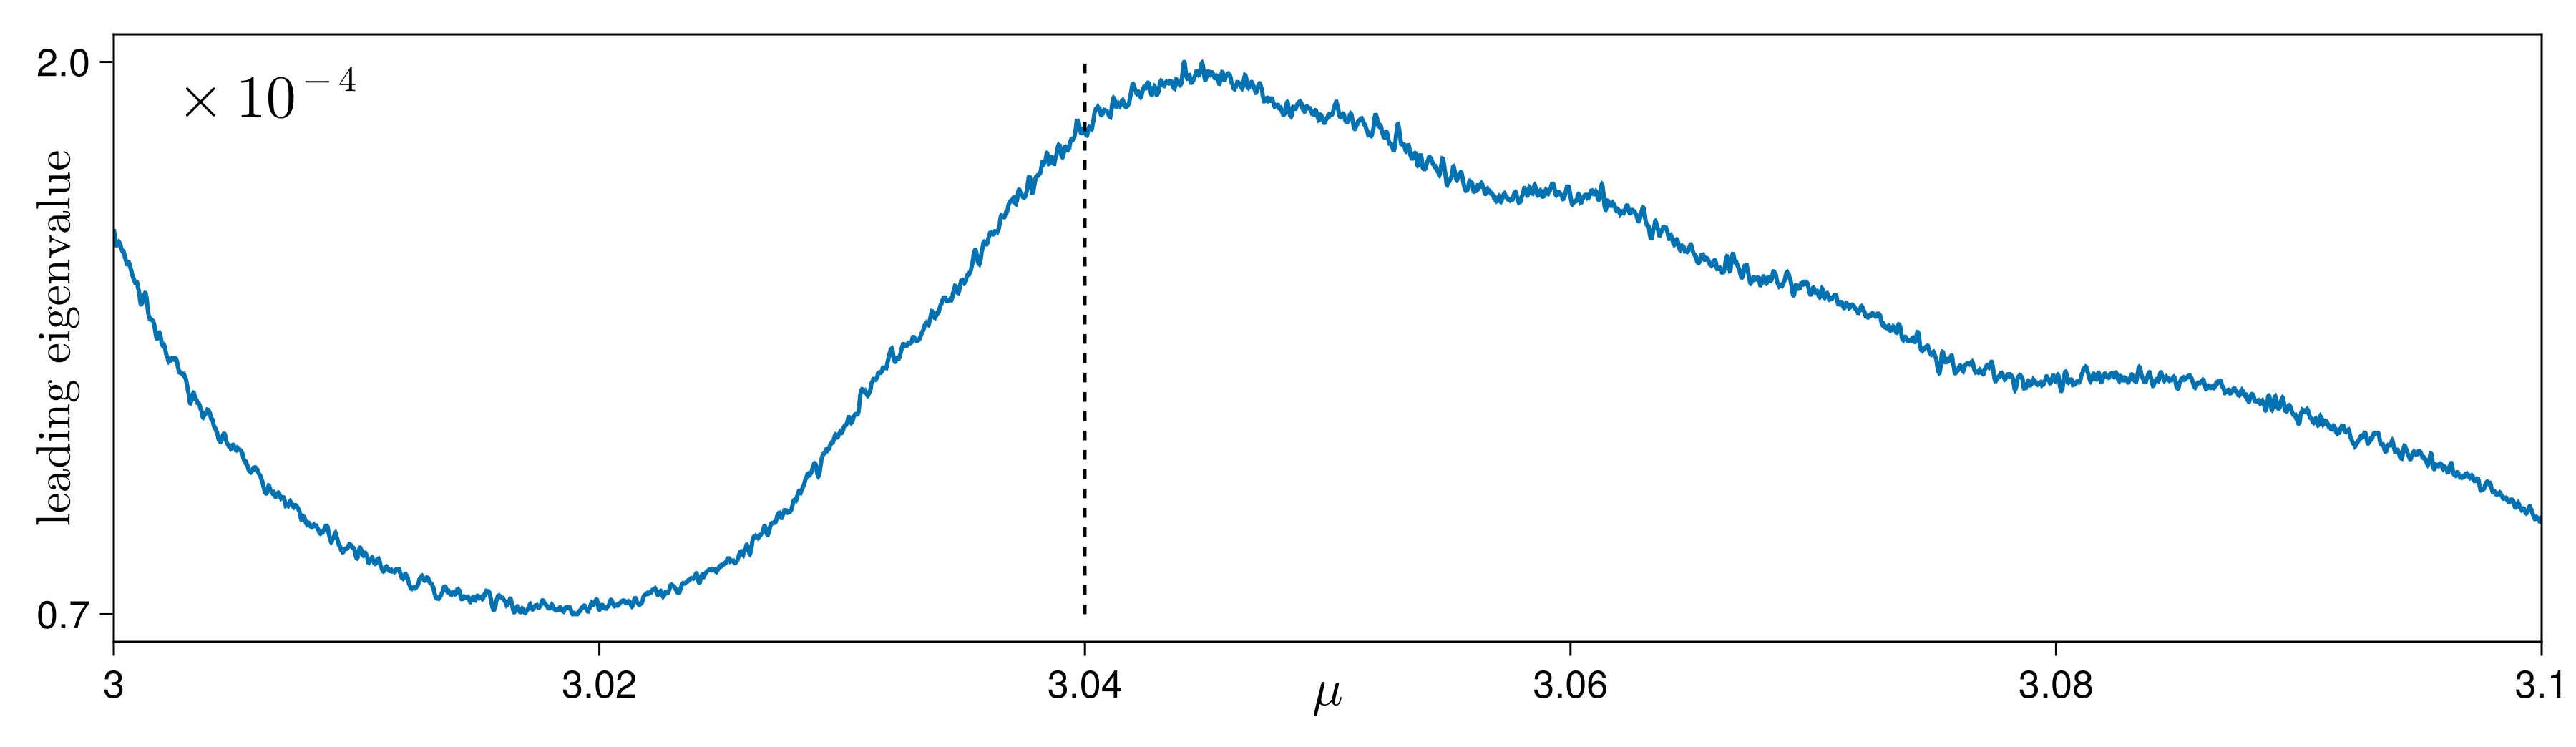
\includegraphics[keepaspectratio, width = \linewidth]{../figures/fig3.8.1.png}
    \end{subfigure}


    \begin{subfigure}[b]{0.11\textwidth}
        \centering 
        
\includegraphics[keepaspectratio, width = \linewidth]{../figures/fig3.8.2.1.png}
    \end{subfigure}
    \hfill
    \begin{subfigure}[b]{0.11\textwidth}
        \centering 
        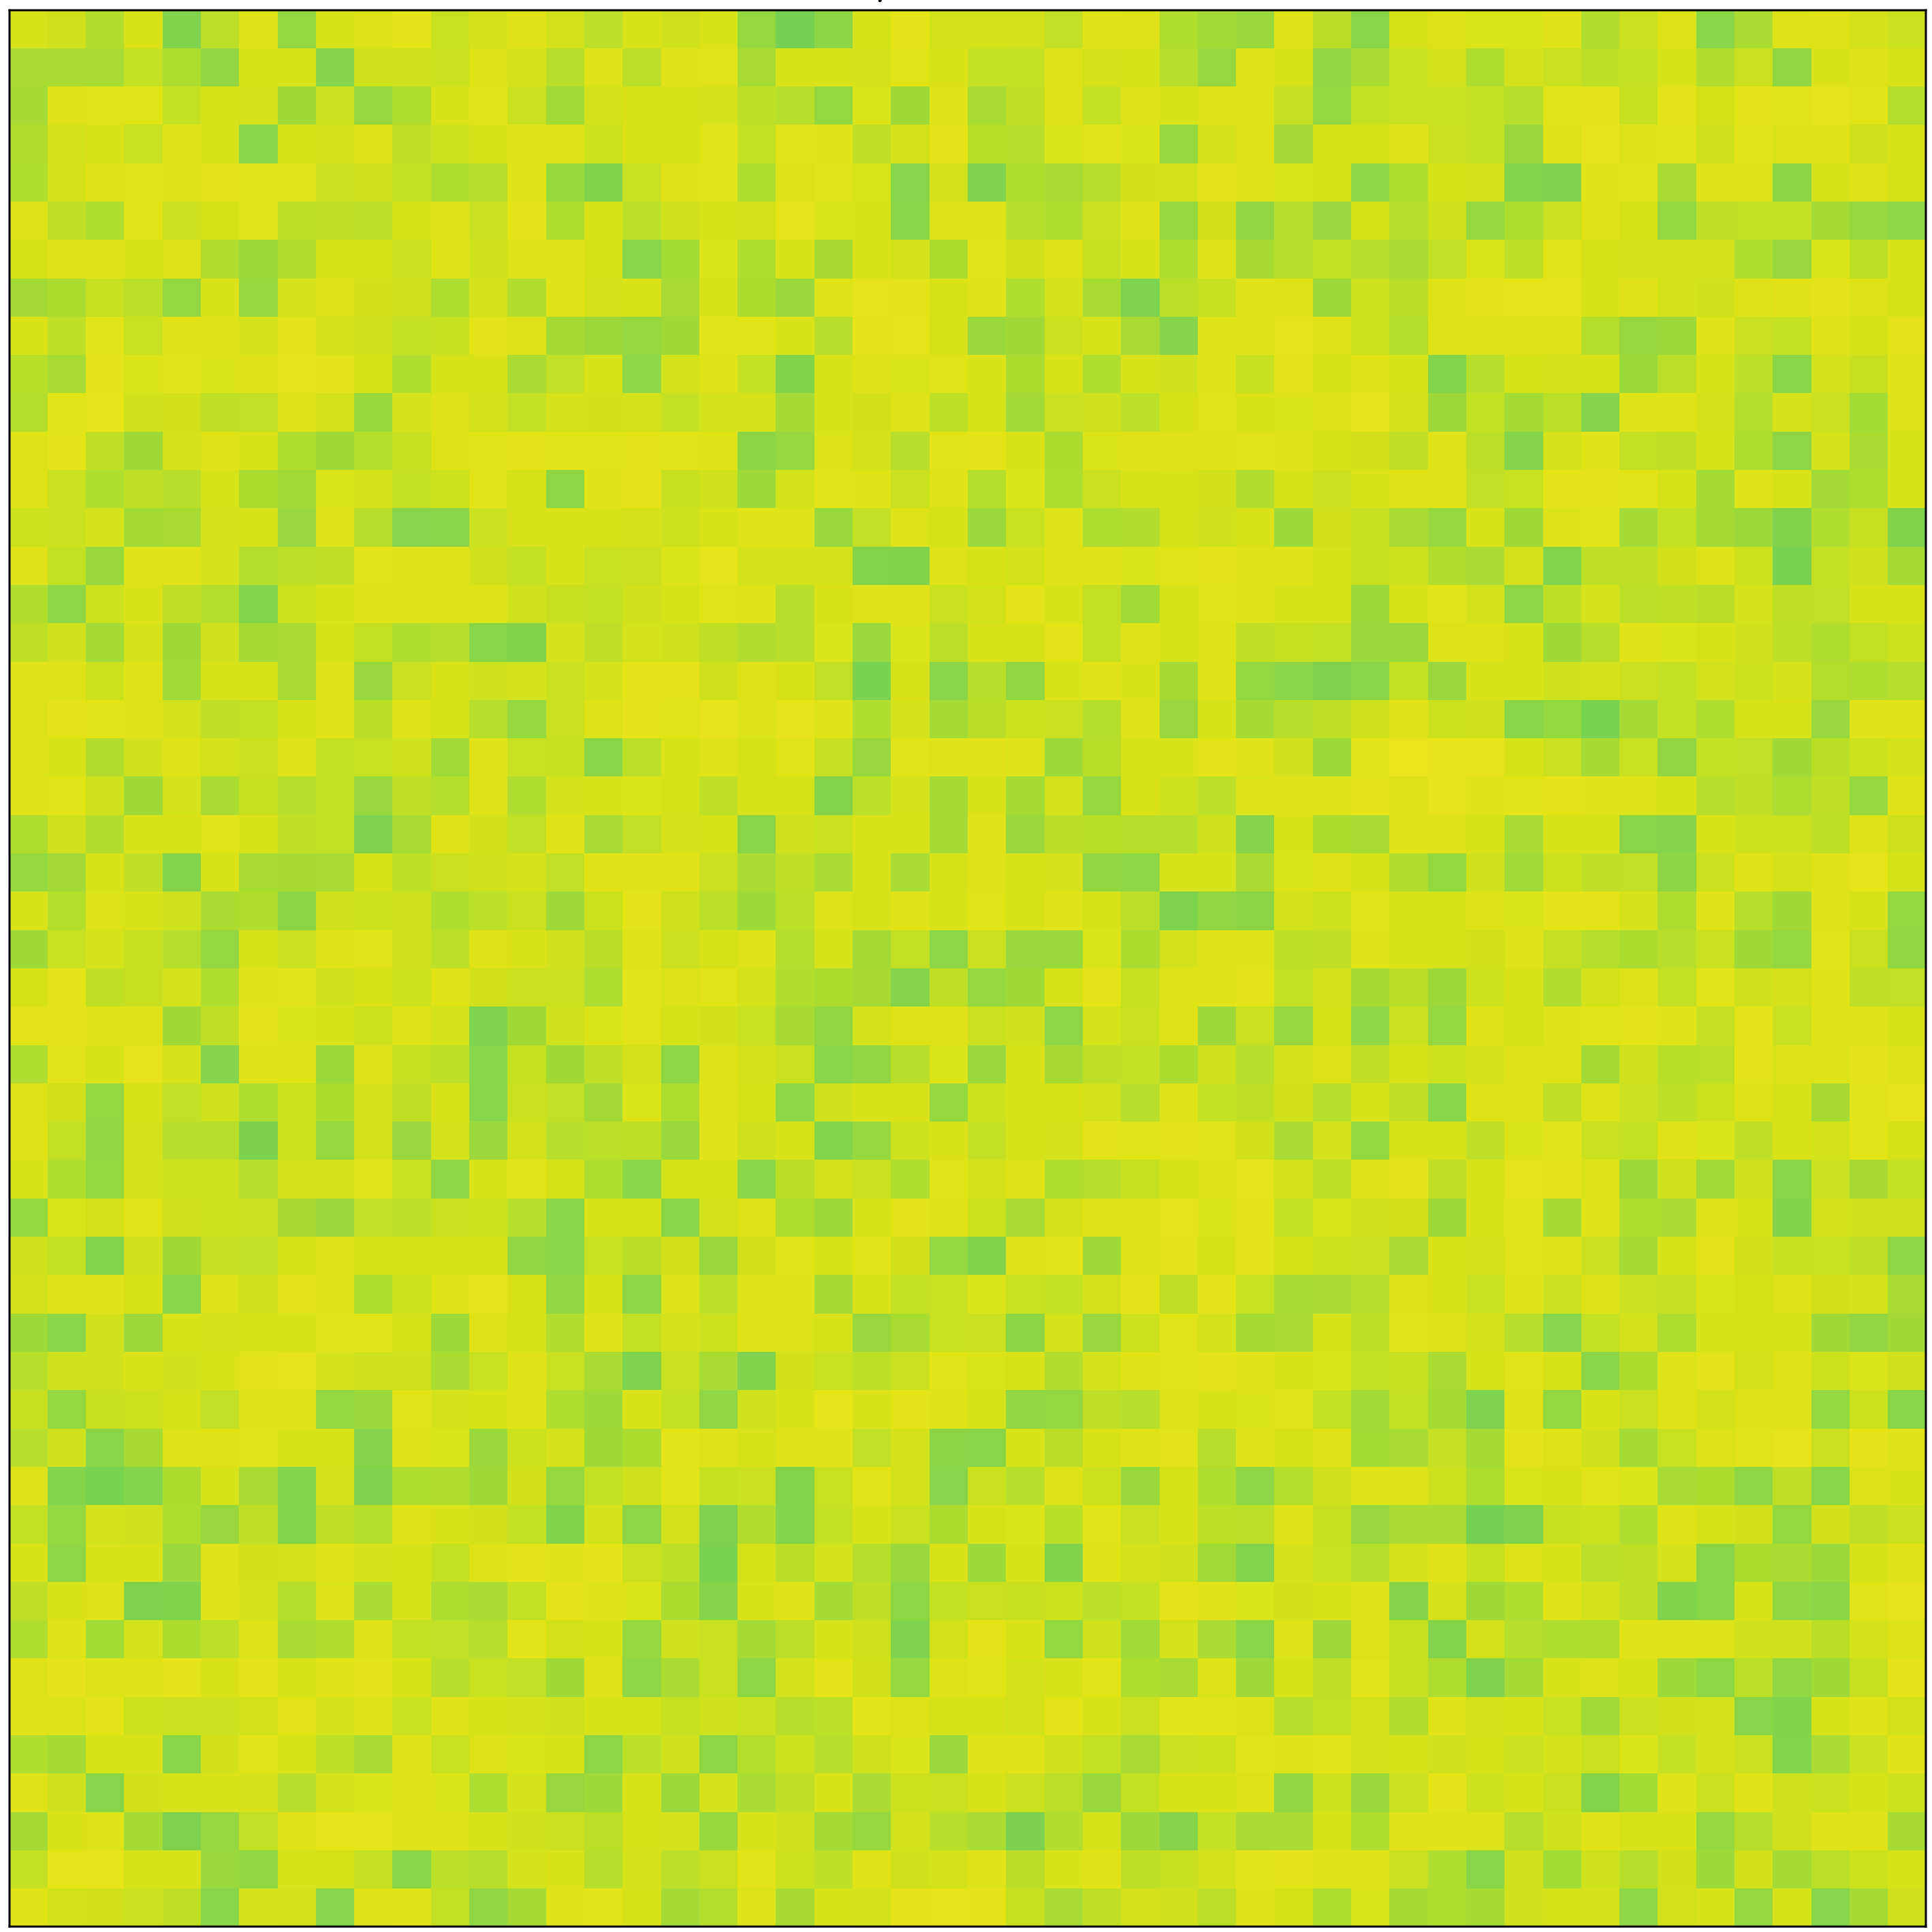
\includegraphics[keepaspectratio, width = \linewidth]{../figures/fig3.8.2.2.png}
    \end{subfigure}
    \hfill
    \begin{subfigure}[b]{0.11\textwidth}
        \centering 
        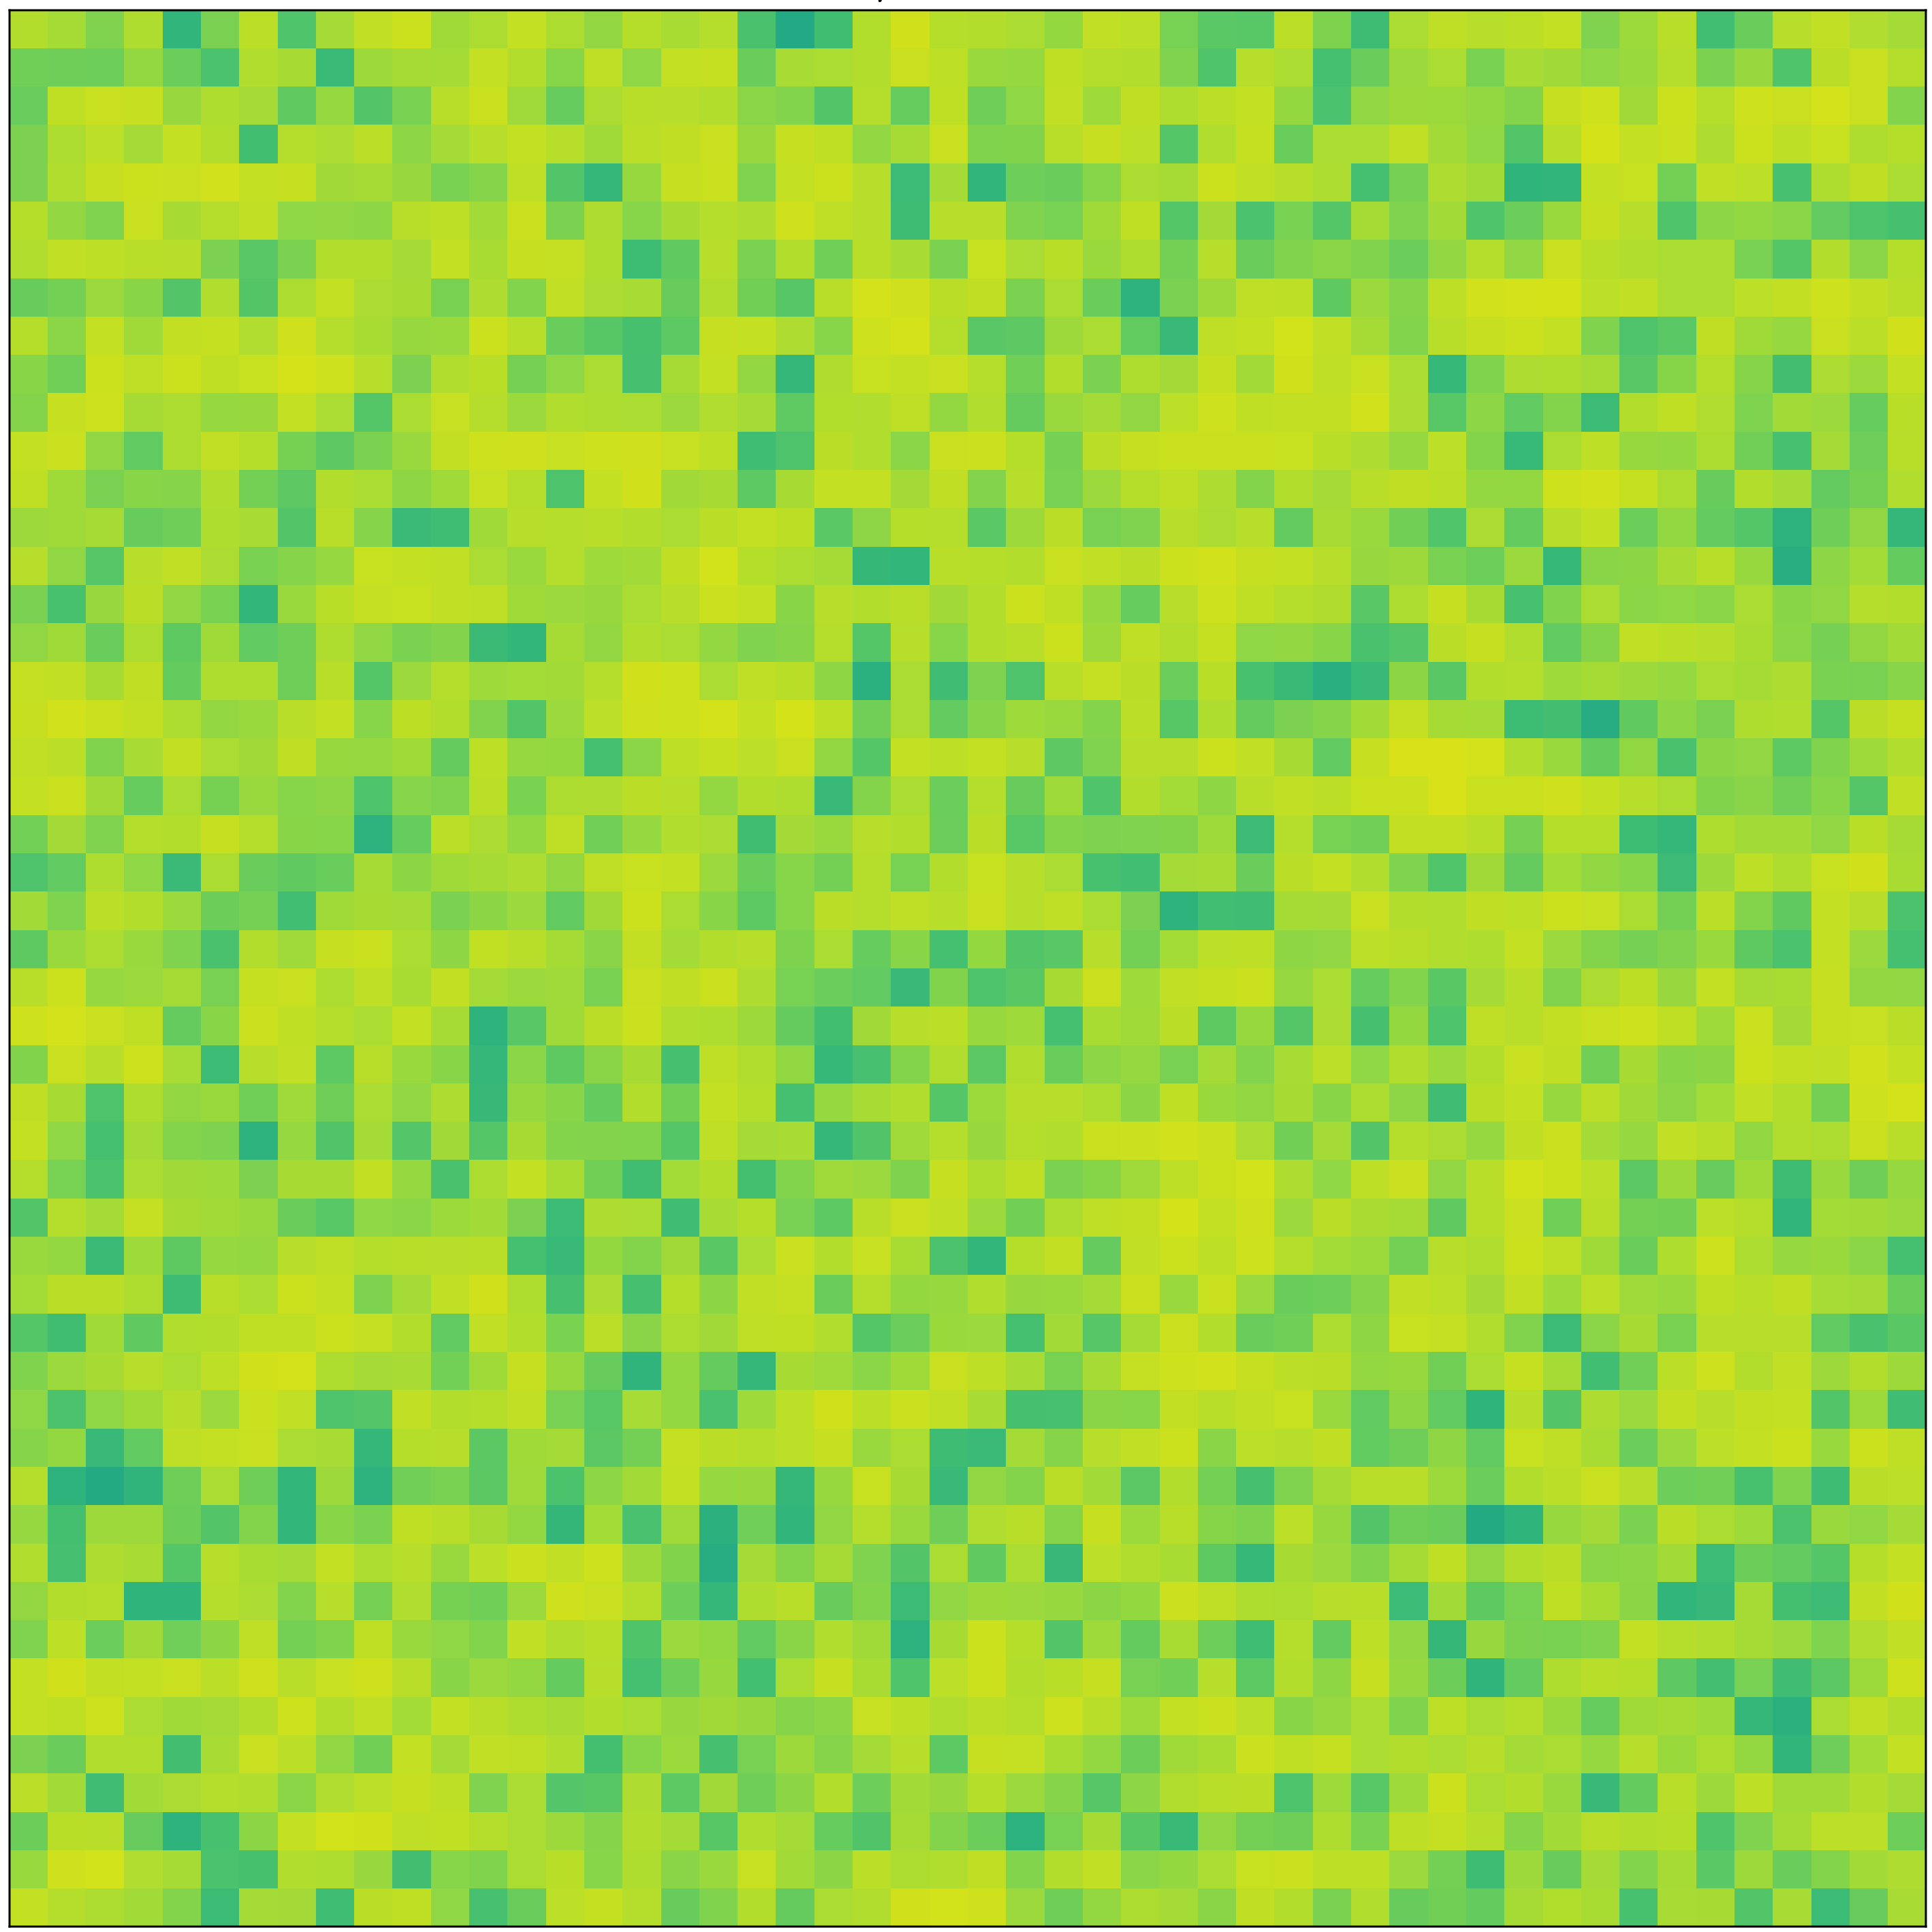
\includegraphics[keepaspectratio, width = \linewidth]{../figures/fig3.8.2.3.png}
    \end{subfigure}
    \hfill
    \begin{subfigure}[b]{0.11\textwidth}
        \centering 
        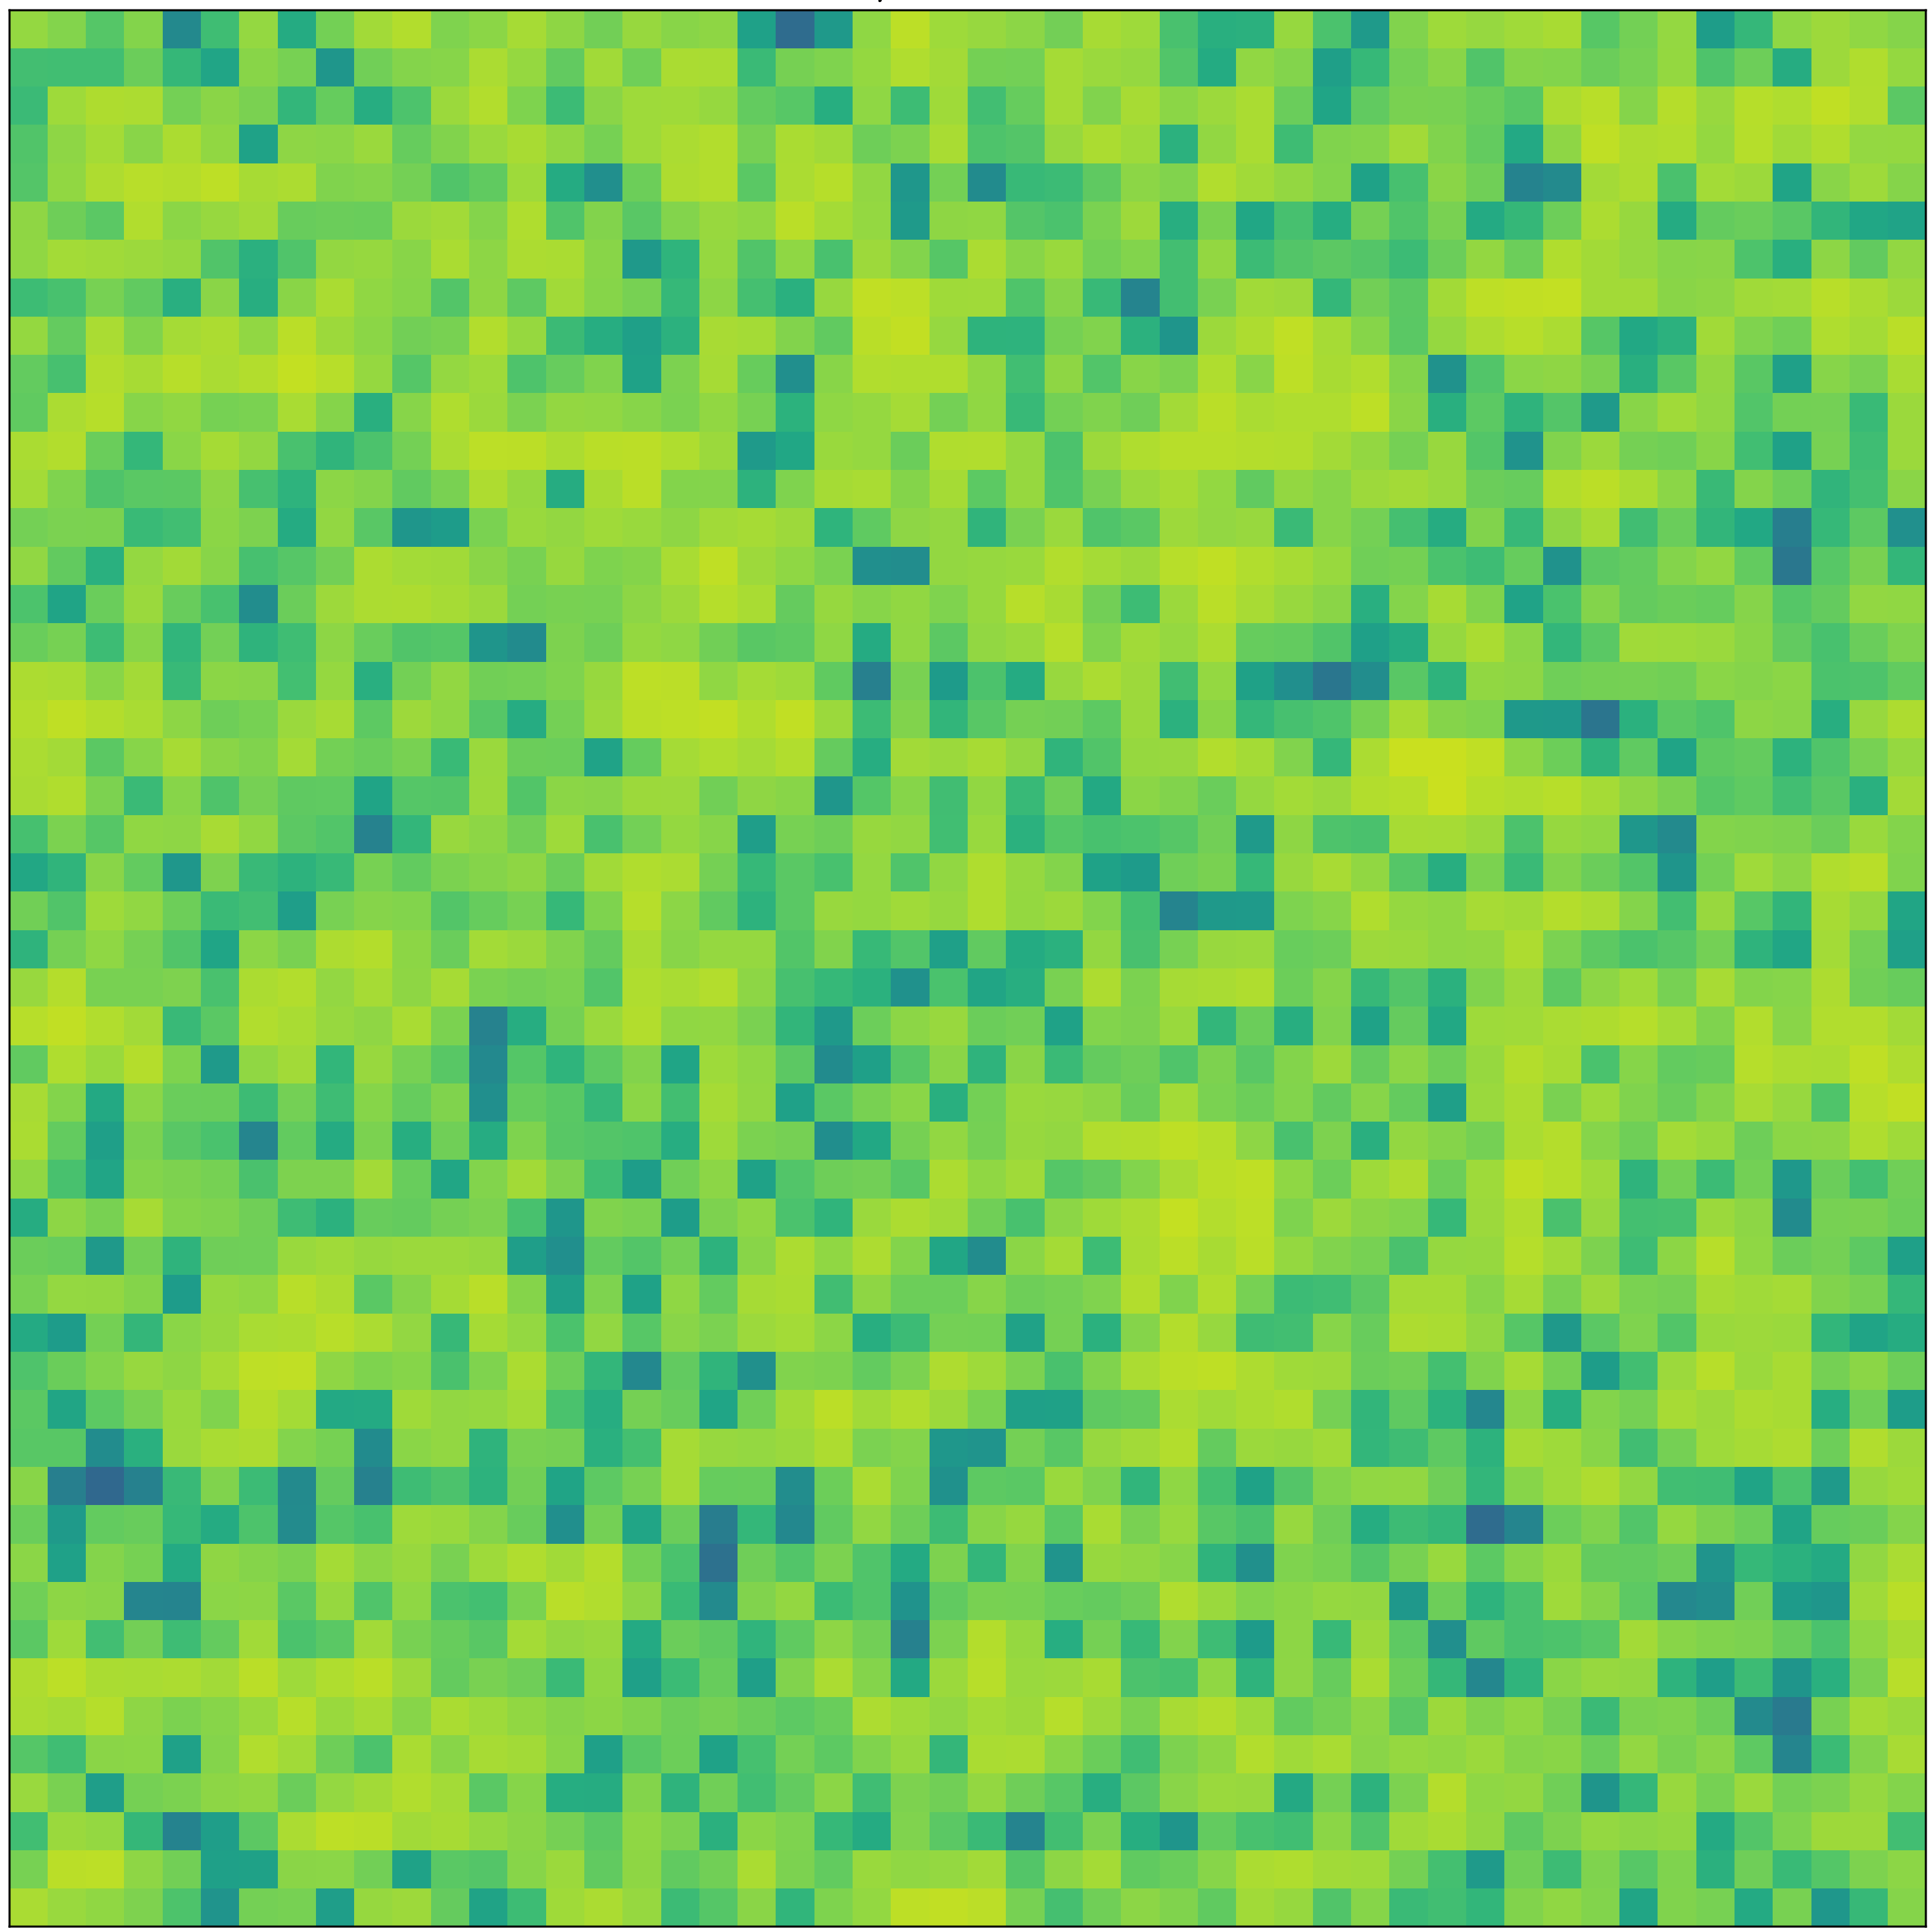
\includegraphics[keepaspectratio, width = \linewidth]{../figures/fig3.8.2.4.png}
    \end{subfigure}
    \hfill
    \begin{subfigure}[b]{0.11\textwidth}
        \centering 
        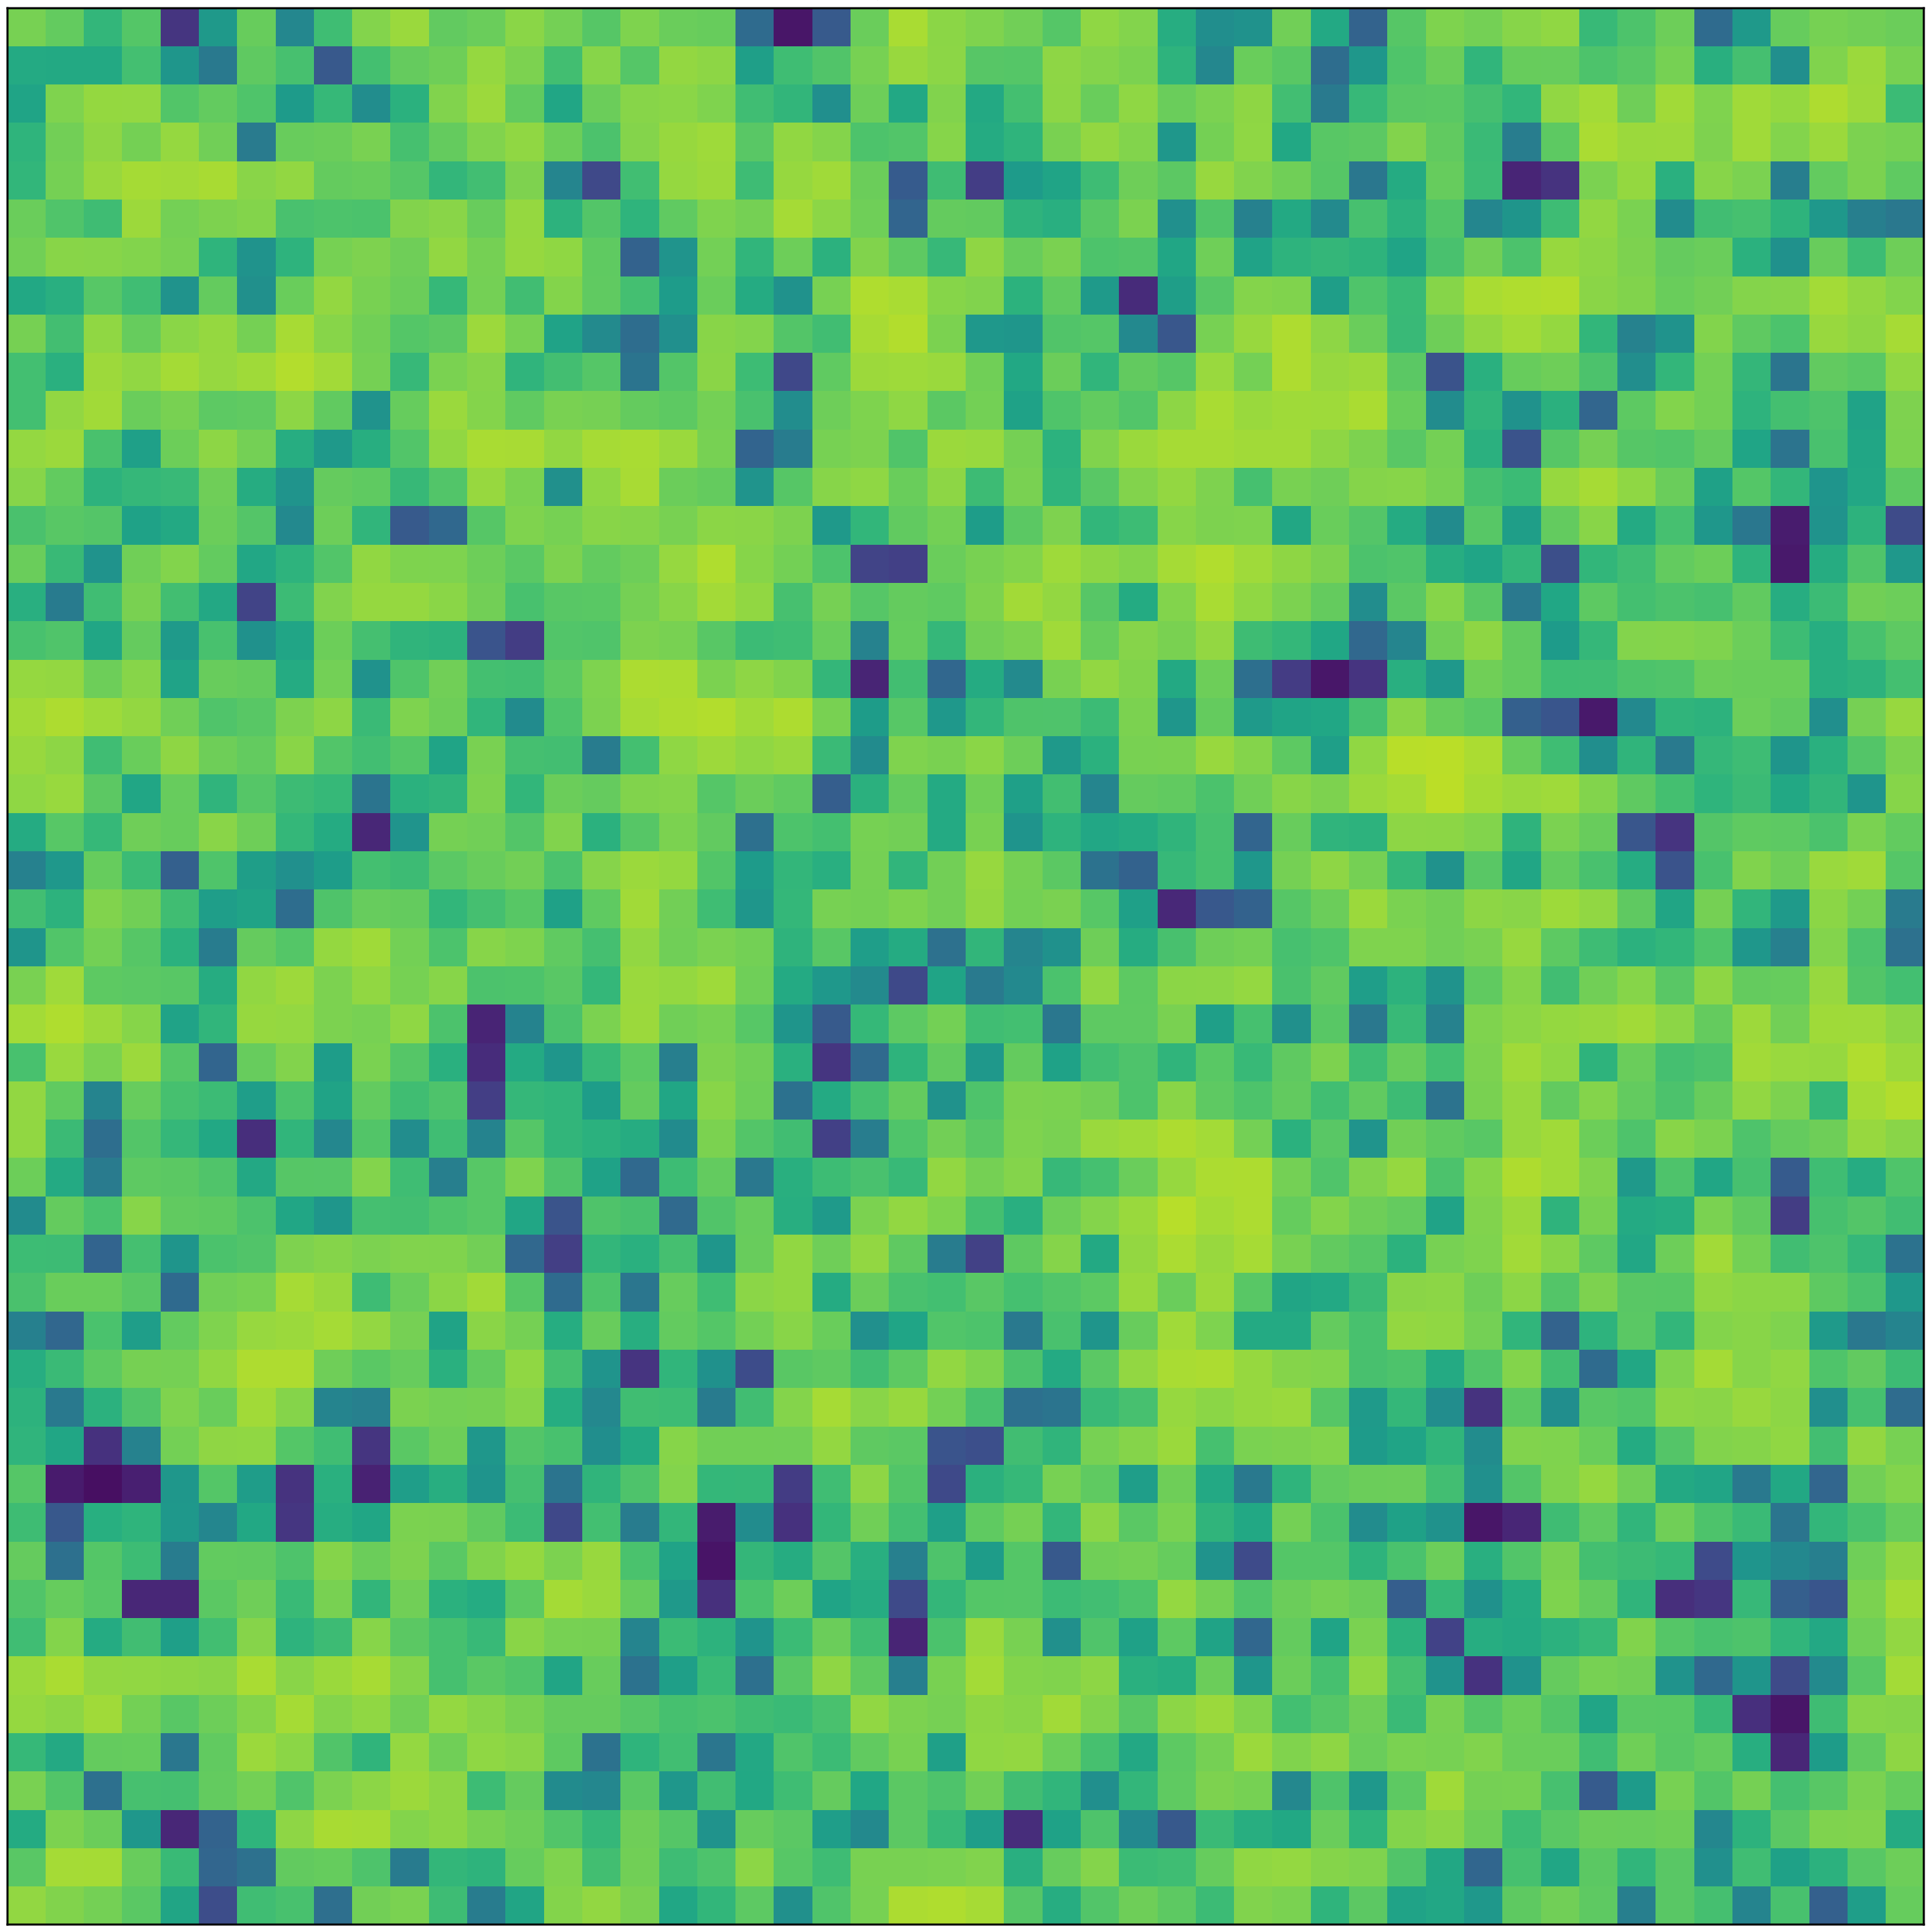
\includegraphics[keepaspectratio, width = \linewidth]{../figures/fig3.8.2.5.png}
    \end{subfigure}
    \hfill
    \begin{subfigure}[b]{0.11\textwidth}
        \centering 
        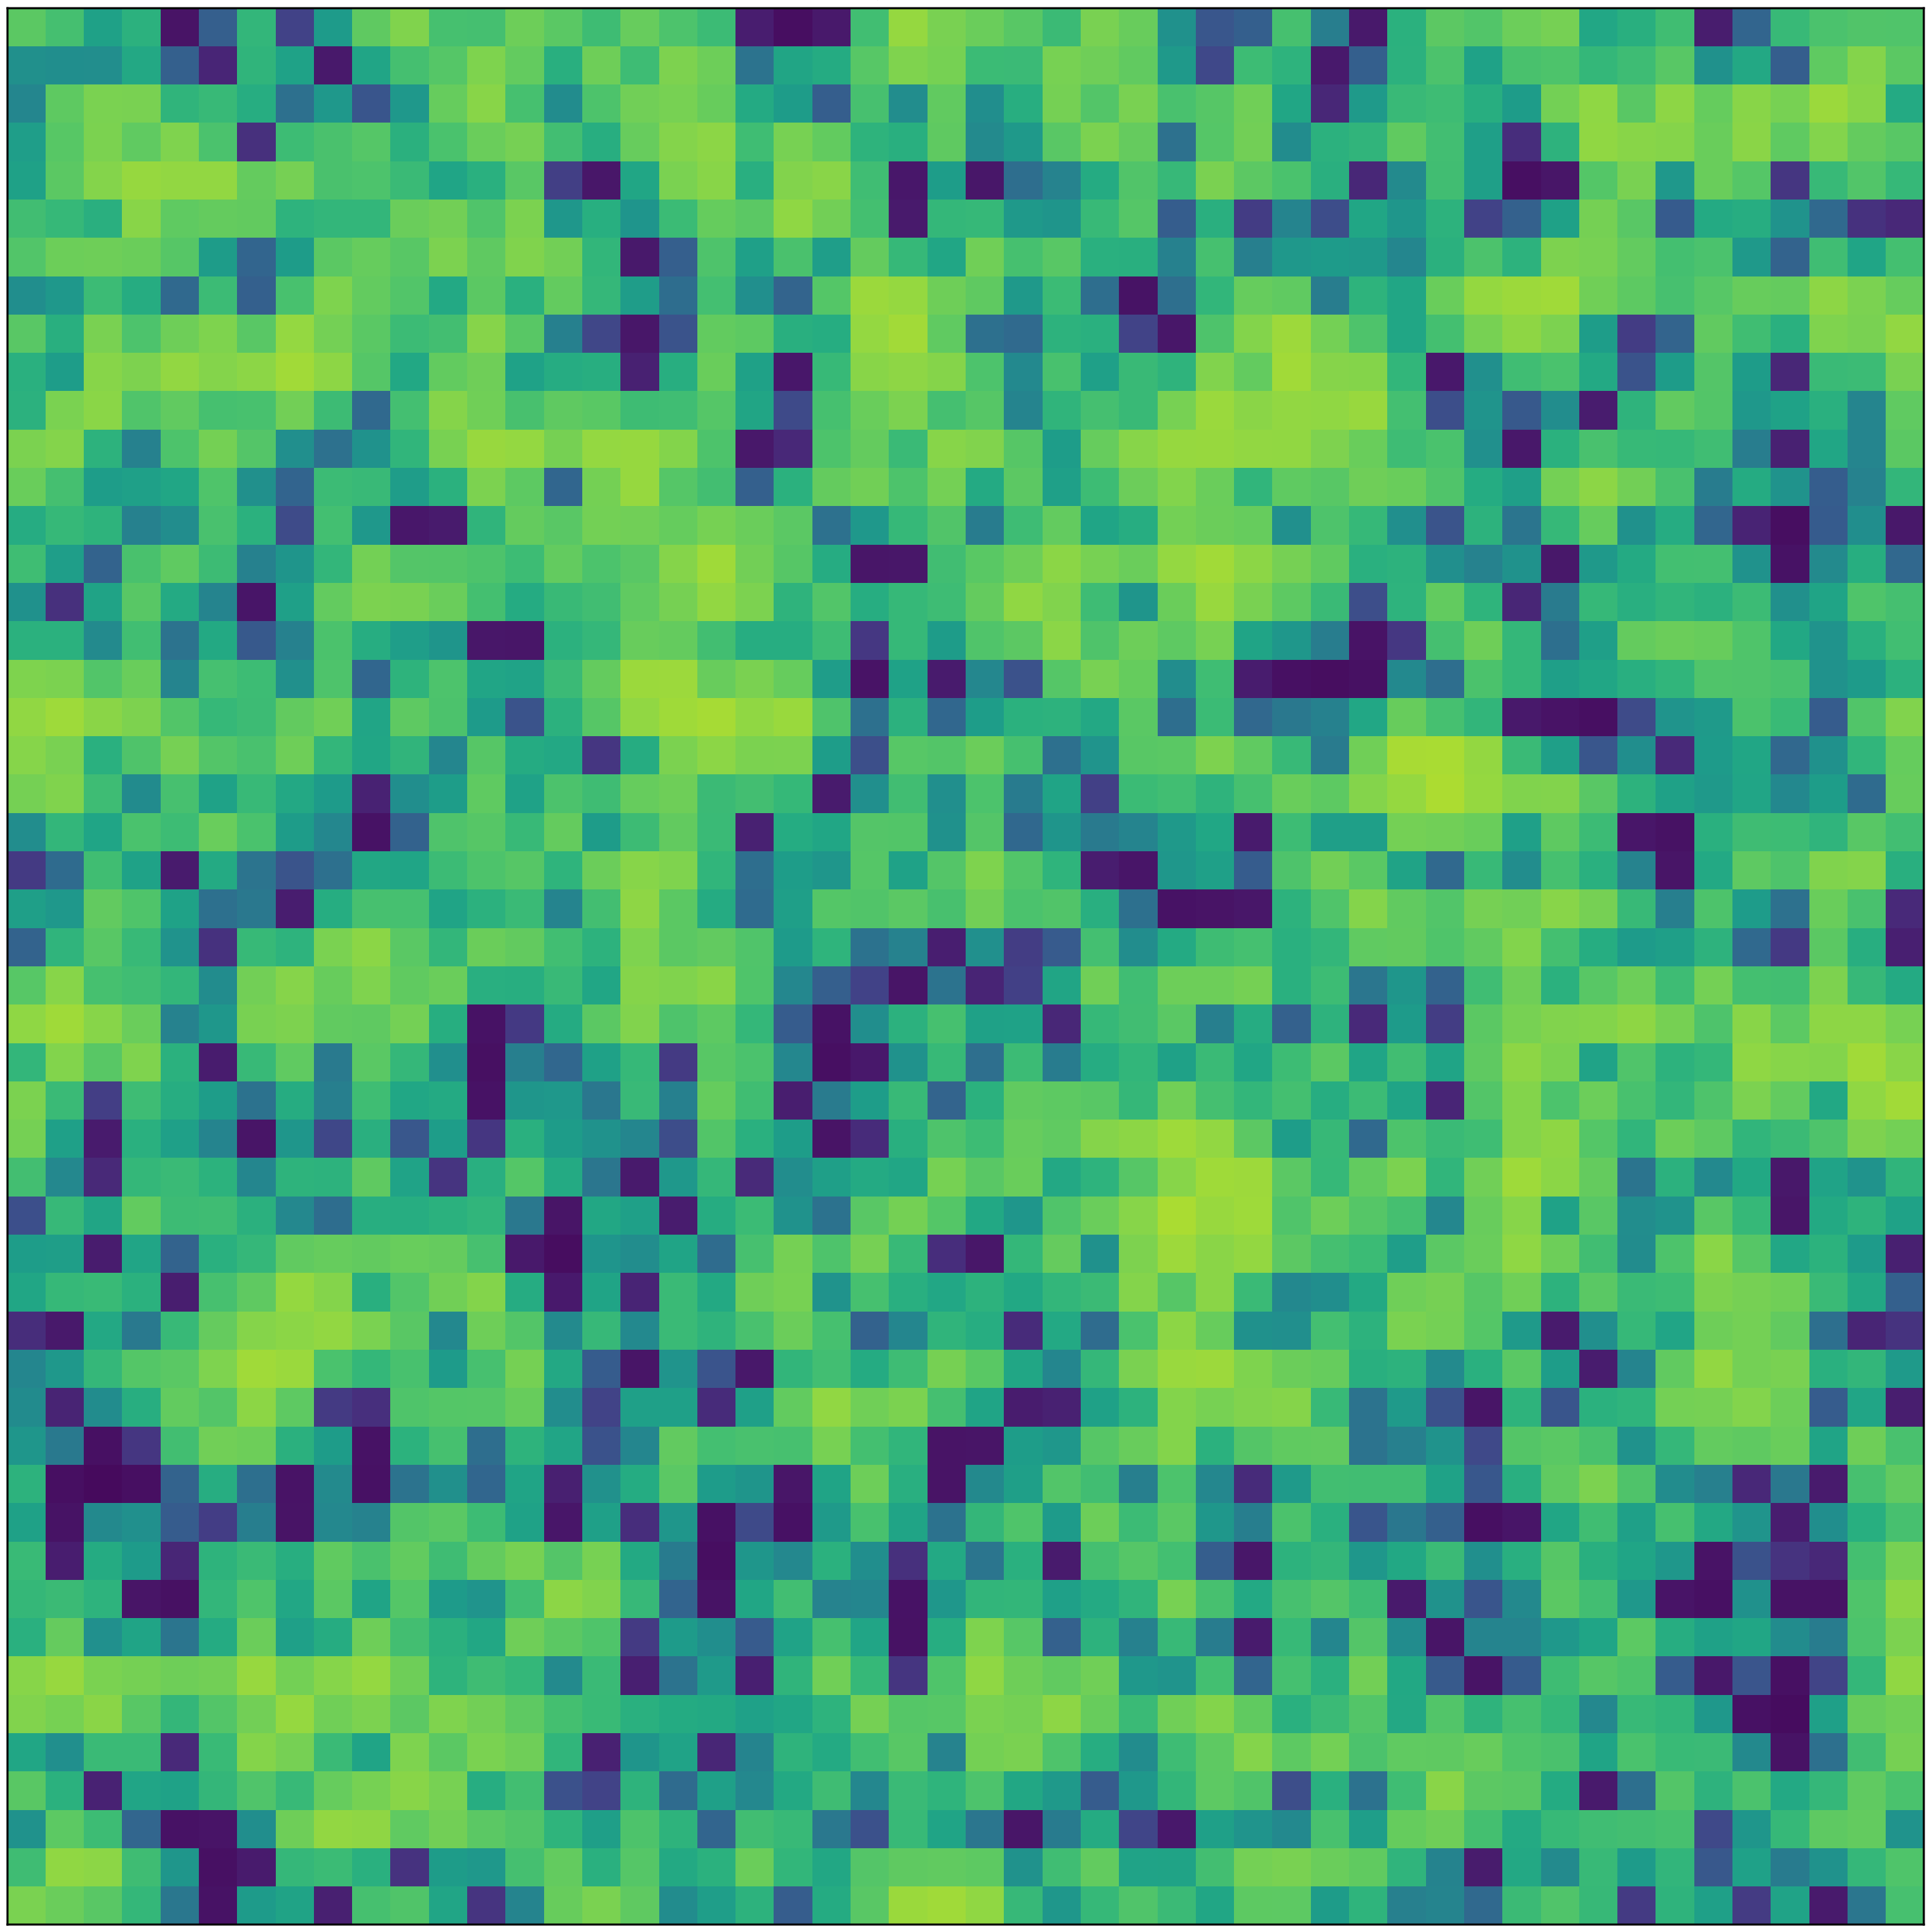
\includegraphics[keepaspectratio, width = \linewidth]{../figures/fig3.8.2.6.png}
    \end{subfigure}
    \hfill
    \begin{subfigure}[b]{0.11\textwidth}
        \centering 
        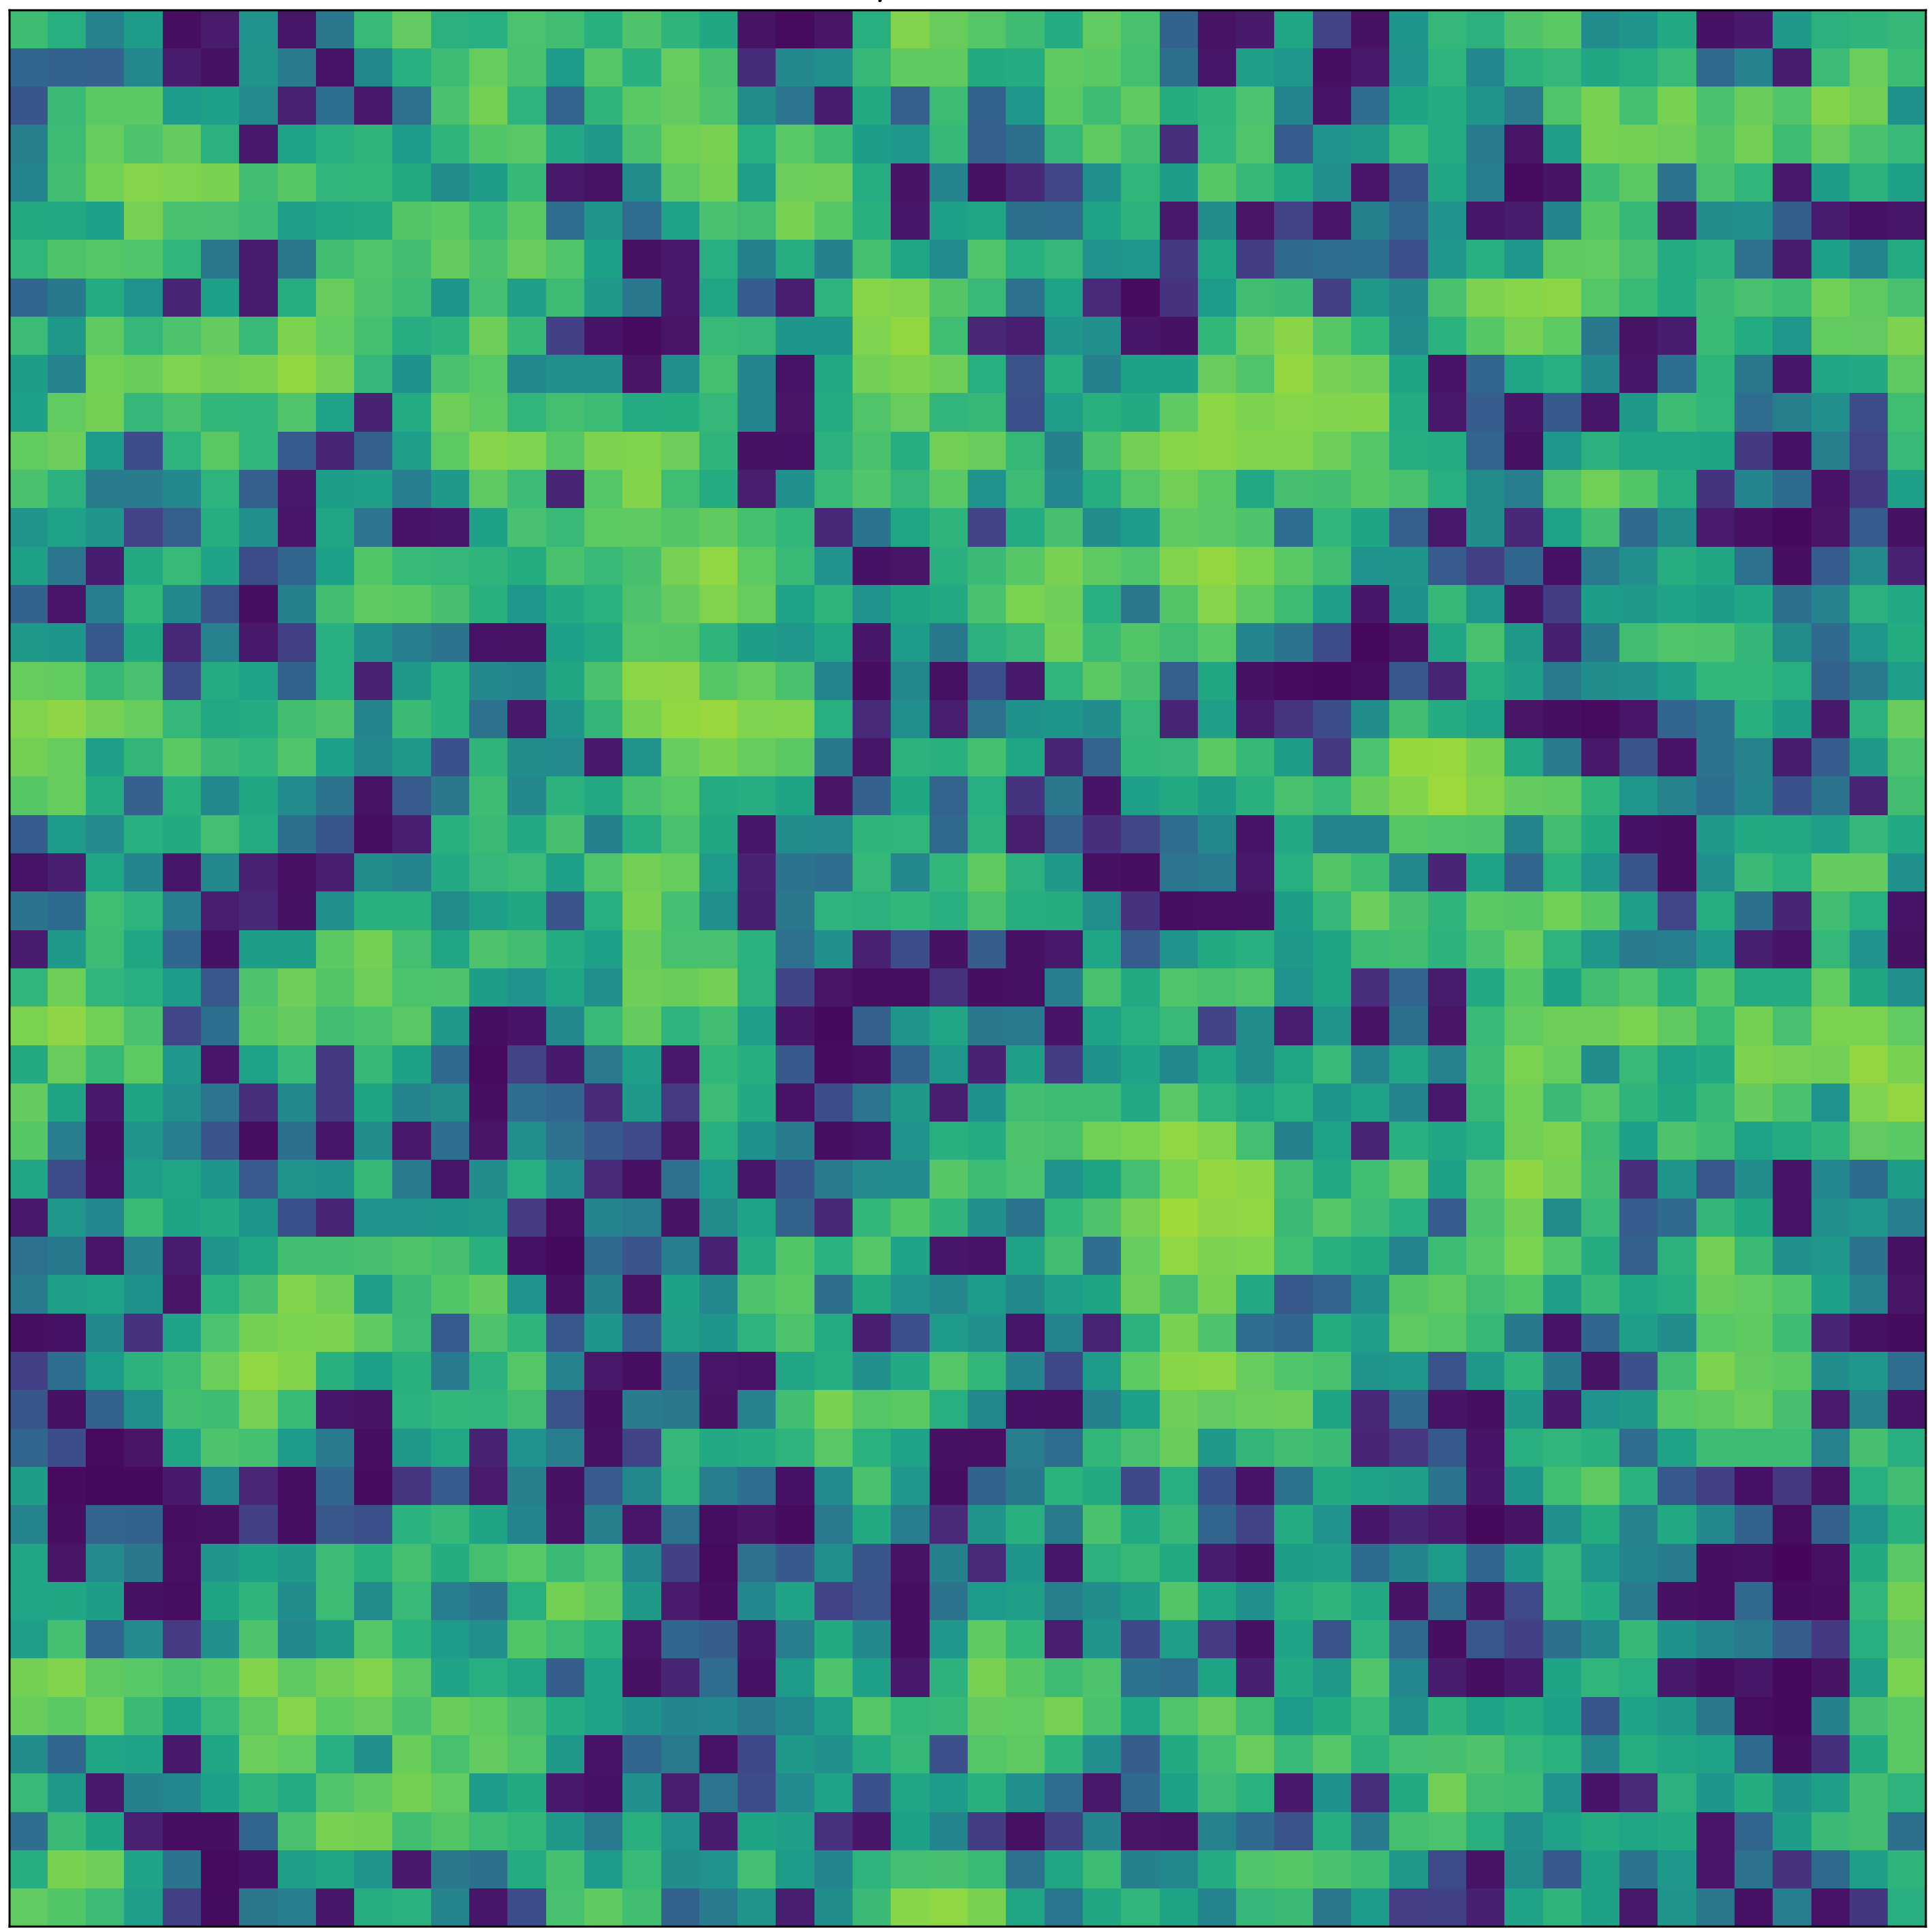
\includegraphics[keepaspectratio, width = \linewidth]{../figures/fig3.8.2.7.png}
    \end{subfigure}
    \hfill
    \begin{subfigure}[b]{0.11\textwidth}
        \centering 
        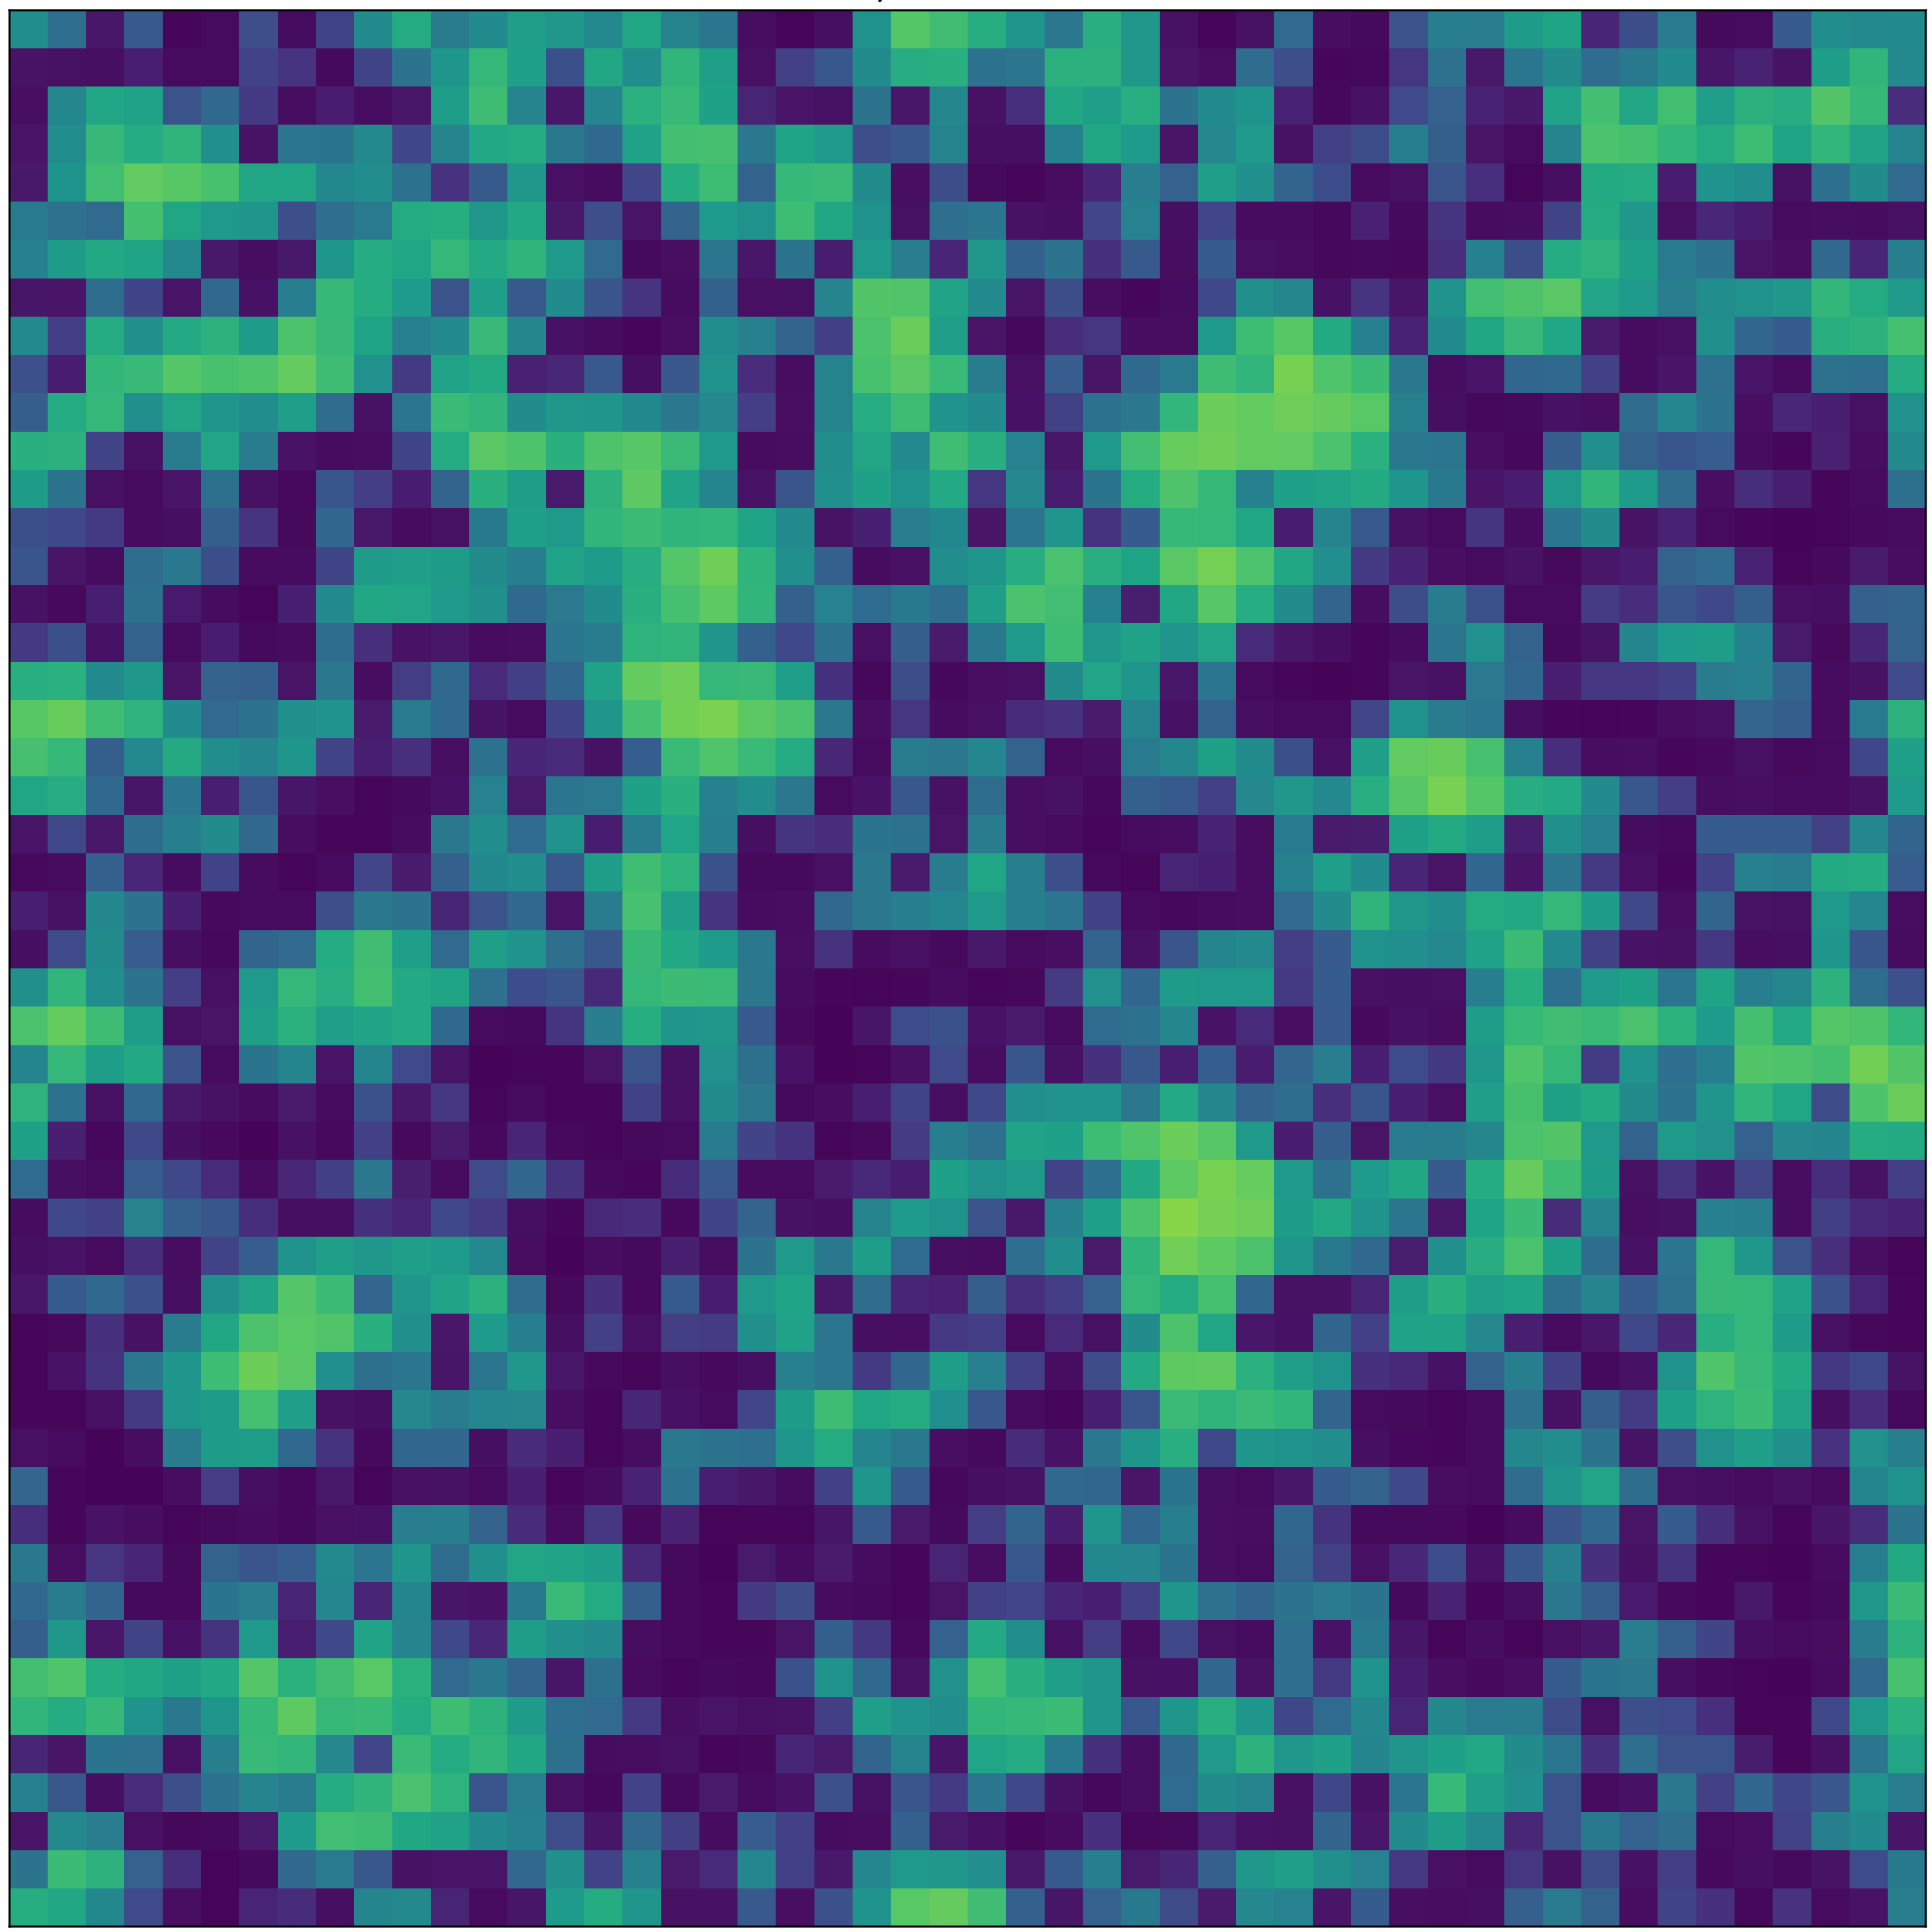
\includegraphics[keepaspectratio, width = \linewidth]{../figures/fig3.8.2.8.png}
    \end{subfigure}
    \caption{Time evolution of the vegetation turbidity LDS on a square $50\times50$ lattice with slow ($\varepsilon=10^{-2}$), linear ramping of the bifurcation parameter, noise level $\sigma=10^{-3}$ and uniform reaction $R=1$ and diffusion $D=0.2$.
The top pannel shows the timeseries of the leading eigenvalue of the covariance matrix assembled over a window of $W=20$ snapshots. 
The dashed vertical line indicates the visual detection of irregular patterns forming in the solution, shown in the bottom panels at increasing timesteps (left to right).}
    \label{fig3.8}
\end{figure}
The fundamental idea behind this analysis is to bring together the spatial and temporal variation of the observables in a (prebefarbly unique) measure that is capable of capturing, with robustness and mathematical interpretability the onset of pattern-formation in spatially extended dynamical systems.
This concept is further investigated in \cite{Donovan22} where the dynamic mode decomposition (DMD) of the Koopman operator linearising the evolution of the reaction-diffusion LDS is employed.
Suppose $\boldsymbol{\mathcal{X}}$ is collecting snapshots from timestep $t_{w}$ to $t_{w+W}$ while in $\boldsymbol{\mathcal{\newprime{X}}}$ we store the snapshots one stride of the sliding window away i.e. capturing the snapshots from $t_{w+S}$ to $t_{(w+S)+W}$.
The DMD will provide us with a more direct and efficient way of capturing CSD and Turing instability by way of approximating the linearisation around the steady-state directly as per the following result.
\begin{theorem}[label=thm3.6]{}{}
     Let $A:\boldsymbol{\mathcal{X}}\to \boldsymbol{\mathcal{\newprime{X}}}$ be a linear operator and $\boldsymbol{\mathcal{X}}\approx \boldsymbol{U}\boldsymbol{\Sigma}\boldsymbol{V}^{T}$ be the singular valued decomposition (SVD) of $\boldsymbol{\mathcal{X}}$, then the spectrum of $\boldsymbol{S}:= \boldsymbol{U}^{T}\boldsymbol{\mathcal{\newprime{X}}}\boldsymbol{V}\boldsymbol{\Sigma}^{-1}$ is the best approximation of the spectrum of A ($\sigma(A)$) and its eigenvectors are also optimally approximated by those of $\boldsymbol{S}$ multiplied from the left by $\boldsymbol{U}$.
\end{theorem}
\begin{proof}
        Here $\boldsymbol{\mathcal{X}}$ will represent a matrix of snapshots of the solution at different timesteps over the square $N-$dimensional lattice (i.e. $N:=n^{2}$) collected across a sliding window of fixed width $W$.
     Since $\boldsymbol{\mathcal{X}}\in \mathbb{R}^{N\times W}$ then the SVD will give us the left and right singular vectors in $\boldsymbol{U}$, $\boldsymbol{V}\in \mathbb{R}^{N\times W}$ respectively while the singular values will be stored along the (main) diagonal of $\boldsymbol{\Sigma}\in \mathbb{R}^{W\times W}$ (which is not the covariance matrix as in the previous case).
     From straightforward algebraic manipulation we get
     \begin{equation*}
          A = \boldsymbol{\mathcal{\newprime{X}}}\boldsymbol{\mathcal{X}}^{-1}\approx \boldsymbol{\mathcal{\newprime{X}}}(\boldsymbol{U}\boldsymbol{\Sigma}\boldsymbol{V}^{T})^{-1}=\boldsymbol{\mathcal{\newprime{X}}}\boldsymbol{V}^{-T}\boldsymbol{\Sigma}^{-1}\boldsymbol{U}^{-1} = \boldsymbol{\mathcal{\newprime{X}}}\boldsymbol{V}\boldsymbol{\Sigma}^{-1}\boldsymbol{U}^{T}\;\Rightarrow\;\boldsymbol{U}^{-1}A \boldsymbol{U}\approx \boldsymbol{U}^{T}\boldsymbol{\mathcal{\newprime{X}}}\boldsymbol{V}\boldsymbol{\Sigma}^{-1}=:\boldsymbol{S}\,,
     \end{equation*}
     where we used the fact that both $\boldsymbol{U}$ and $\boldsymbol{V}$ are orthogonal. The eigendecomposition of $\boldsymbol{S}$ will then give
    \begin{equation*}
         \boldsymbol{U}^{-1}A \boldsymbol{U}\approx \boldsymbol{S}=\boldsymbol{Q}\boldsymbol{\Lambda}\boldsymbol{Q}^{-1}\;\Rightarrow\;A \approx (\boldsymbol{U}\boldsymbol{Q})\boldsymbol{\Lambda}(\boldsymbol{U}\boldsymbol{Q})^{-1}\,.
    \end{equation*}
\end{proof}
As an illustrative example of how the leading eigenvalue of the DMD can provide a prognostic of pattern-formation events here we consider the LDS formulation of a lung ventilation model introduced in \cite{Donovan15}. Again from \eqref{eq3.19} we write
\begin{align}
             \phi(u_{\ell}, u_{\ell\pm1},u_{\ell\pm n};\mu) =&\, \sigma(-r_{\ell})\,, \nonumber \\
            \psi(u_{\ell};\mu) =&\,-u_{\ell} \,,\nonumber
\end{align}
where $\sigma(\theta)=\frac{1}{1+e^{-\theta}}$ is the sigmoid function and 
$$r_{\ell}:=-P_{b}(t)+\mu \frac{k}{u_{\ell}}+P_{b}A(u_{\ell}^{4}+u_{\ell+1}^{4}+u_{\ell-1}^{4}+u_{\ell+n}^{4}+u_{\ell-n}^{4})(1 - 1 - u_{\ell}+ \frac{3}{2}(1-u_{\ell})^{2})\,,$$
with $P_{b}(t):=\frac{P_{b}(0)N}{\sum_{\ell=1}^{N}u_{\ell}^{4}}$. Notice that this last term enforces global-coupling of the lattice sites alongside the traditional local, nearest-neighbour interactions of the discrete diffusion operator.
Finally the remaining homogeneous constants are set to $k=14.1$, $A=0.63$, $P_{i}=0.96$, $P_{b}(0)=7.25$.
In Figure \ref{fig3.10} below we report the detection of the proposed spatio-temporal EWS for this model.
\begin{figure}[H]
    \centering 
    \begin{subfigure}[b]{\textwidth}
        \centering 
        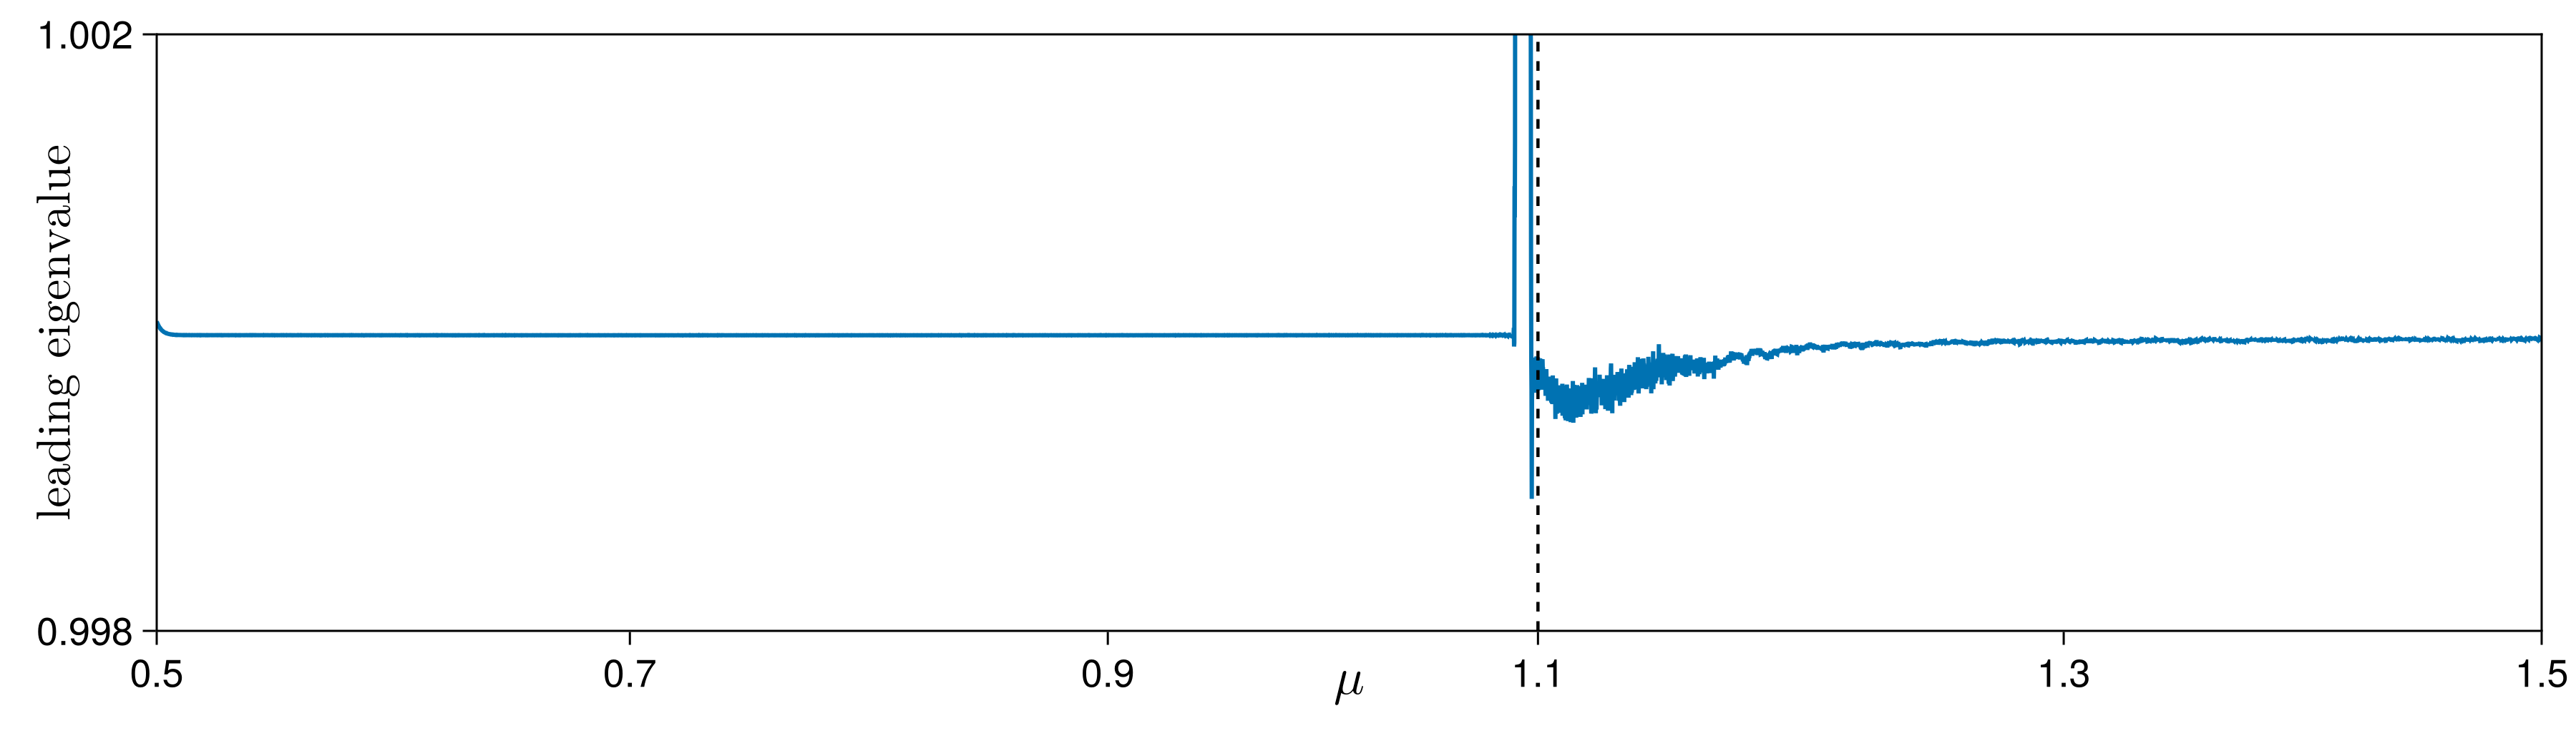
\includegraphics[keepaspectratio, width = \linewidth]{../figures/fig3.9.1.png}
    \end{subfigure}


    \begin{subfigure}[b]{0.11\textwidth}
        \centering 
        
\includegraphics[keepaspectratio, width = \linewidth]{../figures/fig3.9.2.1.png}
    \end{subfigure}
    \hfill
    \begin{subfigure}[b]{0.11\textwidth}
        \centering 
        
\includegraphics[keepaspectratio, width = \linewidth]{../figures/fig3.9.2.2.png}
    \end{subfigure}
    \hfill
    \begin{subfigure}[b]{0.11\textwidth}
        \centering 
        
\includegraphics[keepaspectratio, width = \linewidth]{../figures/fig3.9.2.3.png}
    \end{subfigure}
    \hfill
    \begin{subfigure}[b]{0.11\textwidth}
        \centering 
        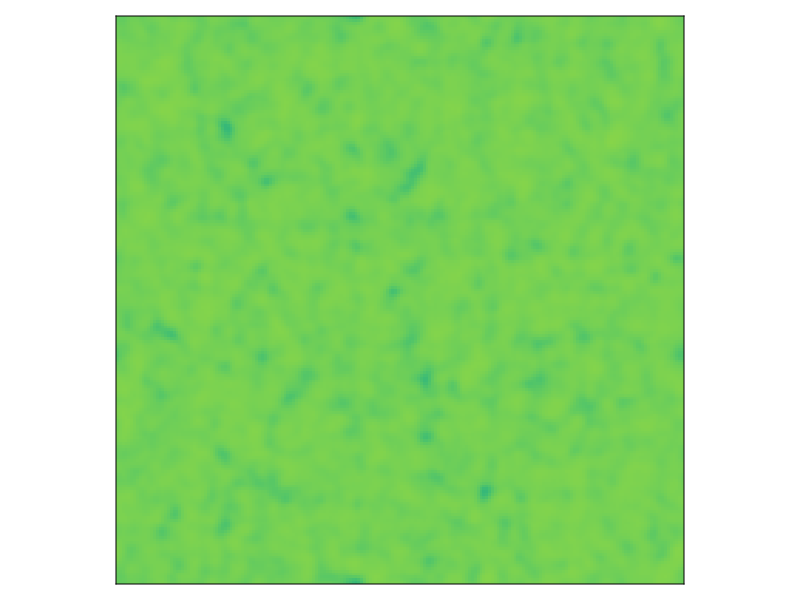
\includegraphics[keepaspectratio, width = \linewidth]{../figures/fig3.9.2.4.png}
    \end{subfigure}
    \hfill
    \begin{subfigure}[b]{0.11\textwidth}
        \centering 
        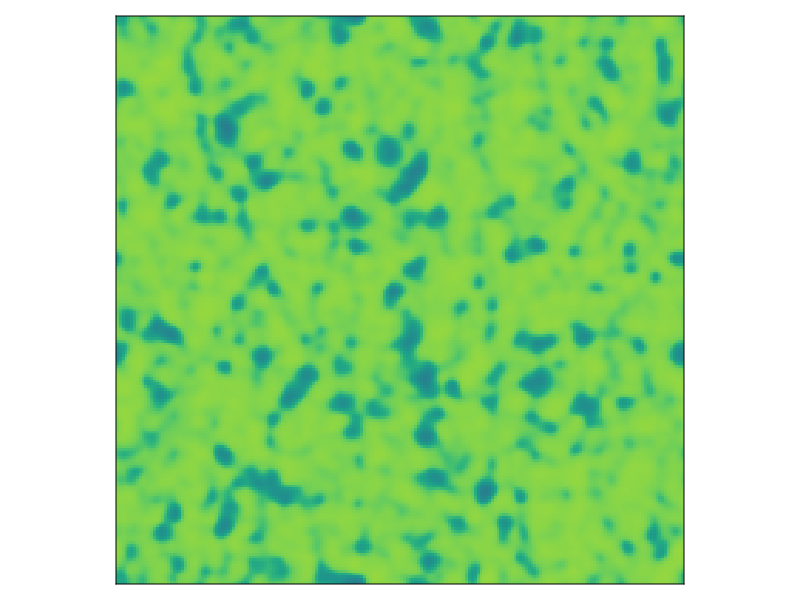
\includegraphics[keepaspectratio, width = \linewidth]{../figures/fig3.9.2.5.png}
    \end{subfigure}
    \hfill
    \begin{subfigure}[b]{0.11\textwidth}
        \centering 
        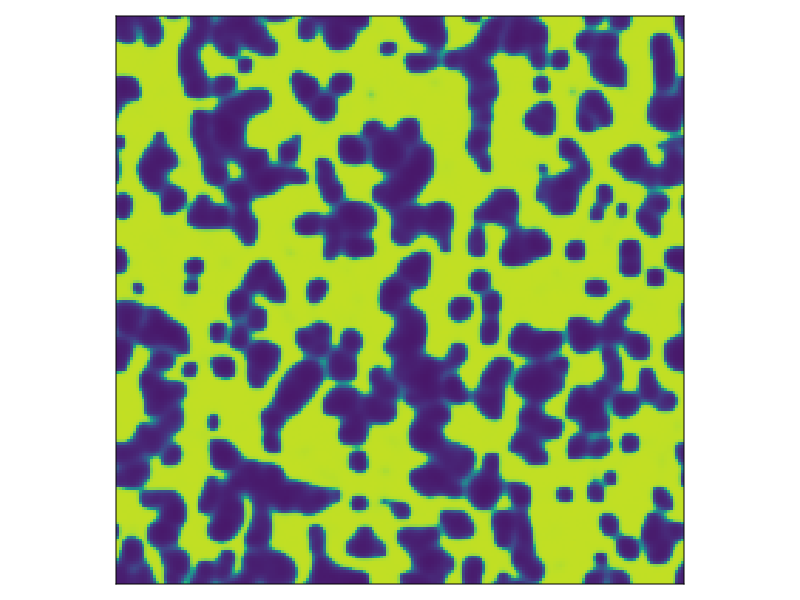
\includegraphics[keepaspectratio, width = \linewidth]{../figures/fig3.9.2.6.png}
    \end{subfigure}
    \hfill
    \begin{subfigure}[b]{0.11\textwidth}
        \centering 
        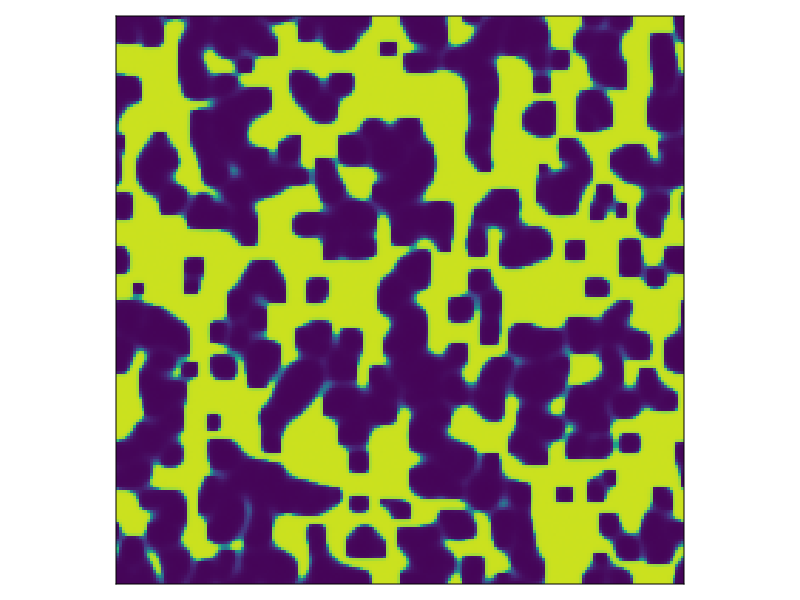
\includegraphics[keepaspectratio, width = \linewidth]{../figures/fig3.9.2.7.png}
    \end{subfigure}
    \hfill
    \begin{subfigure}[b]{0.11\textwidth}
        \centering 
        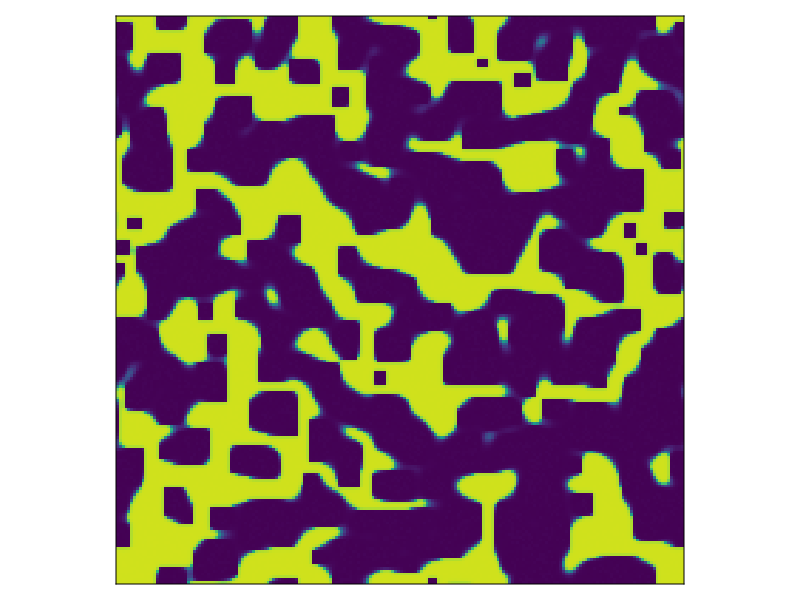
\includegraphics[keepaspectratio, width = \linewidth]{../figures/fig3.9.2.8.png}
    \end{subfigure}
    \caption{Time evolution of the lung ventilation LDS on a square $300\times300$ lattice with slow ($\varepsilon=10^{-2}$), linear ramping of the parameter and noise level $\sigma=10^{-3}$. 
    In the top panel the leading mode of the DMD is reported, showing an abrupt upward burst shortly before the formation of patterns (dashed vertical line). 
In the bottom pannel several snapshots increasing timesteps are reported.}
    \label{fig3.9}
\end{figure}
\subsection{A comprehensive catalogue of spatio-temporal early-warning signals}\label{subsec2.3}
The two indicators of pattern-forming tipping events discussed above are but among the latest entries of a much larger ecosystem of EWS that have been proposed throughout the past two decades. 
Their distinctive property w.r.t. the rest of the earlier measures is that they both combine spatial and temporal information rather than looking at either dimensions individually.
As addressed in the earlier literature review, the discovery and characterisation of tipping events was preceeded by the observation of critical phenomena s.a. CSD and flickering whose measurement through statistical and dynamical indicators become later EWS.
As discussed in the previous Chapter, the robustness of the signals of these precursors is of uttermost importance.
Specifically an optimal EWS of tipping events should address: 
\begin{itemize}
     \item the existence (or lack thereof) of a sound mathematical framework linking the properties and structure of the models exhibiting a tipping event with the underlying theorised or observed phenomena (i.e. CSD, flickering etc...);
     \item a reasonably wide scope of applicability (or degree of universality) to different natural systems modelled by the same mechanism (e.g. reaction-diffusion equations);
     \item the sensitivity of the indicator to downsampling and other practical limitations in the monitoring of complex real-world systems (s.a. climate change, ecosystem collapse, onset of asthma etc...);
     \item the reliance of the methods detecting the signal on single and multivariate timeseries analysis, including detrending and other preprocessing techniques.
\end{itemize}
Addressing how robust a spatio-temporal EWS is w.r.t. the aforementioned metrics is arguably among the most important tasks ahead in the discovery and characterisation of catastrophic regime shifts. 
To conclude this Chapter, here we limit ourselves in categorizing the indicators of the precursors discussed in the literature review.
A tabulated list of indicators is not new and as a matter of fact we found $5$ works \cite{Lenton11, Dakos12a, Scheffer12, Kefi14, Scheffer15} published in the first half of the 2010s compiling a comprehensive collection of the EWS being proposed until then and their connections to the relevant precursors.
Remarkably \cite{Scheffer15} was also accompained by the creation of a website\footnote{\url{https://www.early-warning-signals.org/}} collecting and detailing all the progresses that have been done insofar in the detection of both ad-hoc and generic EWS.
In Table \ref{tab2.1} below we merge these lists by selecting only those indicators that have shown promises of robustness to some degree while enriching them with newer signals proposed after the publication of the aforementioned papers.
We remark that the discovery of critical phenomena preceeding a critical transition and characterising them using indicators has been an ongoning effort by multiple communities with a strong focus in the ecological and climate sciences.
This means that the mathematical ground upon which many of those precursors are based varies greatly, from semi-rigorous and well-developed frameworks for idealised cases \cite{Kuehn11, Kuehn13} to more pragmatic, data-driven and intuition-based indicators of experimental monitorings for scientific applications \cite{Scheffer09,Lenton11}.
\begin{table}[H]
\centering
\begin{tabular}{|lll|}
 \hline
 Indicator & Phenomenon & First proposed \\
 \hline
 recovery time & CSD & 1995 (\cite{Ives95}) \\
 \rowcolor{lightgray} spectral reddening & CSD & 2003 (\cite{Kleinen03}) \\
 autoregressive model fitting & CSD & 2004 (\cite{Held04}) \\
 \rowcolor{lightgray} lag-1 autocorrelation & CSD & 2004 (\cite{Held04}) \\
 \textbf{size distribution of patches} & Turing instability & 2004 (\cite{Rietkerk04}) \\
 \rowcolor{lightgray} \textbf{spatial variance} & CSD, flickering, Turing instability & 2005 (\cite{Oborny05}) \\
 \rowcolor{lightgray} variance & CSD, flickering & 2006 (\cite{Carpenter06}) \\
 detrended fluctuation analysis & CSD & 2007 (\cite{Livina07}) \\
 \rowcolor{lightgray} \textbf{leading eigenvalue of the covariance} & CSD, Turing instability & 2008 (\cite{Carpenter08}) \\
 skewness & flickering & 2008 (\cite{Guttal08}) \\
 mean exit time & CSD & 2008 (\cite{Guttal08}) \\
 kurtosis & flickering & 2009 (\cite{Biggs09}) \\
 \textbf{spatial skewness} & flickering, Turing instability & 2009 (\cite{Guttal09}) \\
 \rowcolor{lightgray} \textbf{spatial spectral reddening} & CSD, Turing instability & 2010 (\cite{Carpenter10}) \\
 \rowcolor{lightgray} \textbf{spatial correlation} & CSD, \newline Turing instability & 2010 (\cite{Drake10}) \\
 potential analysis & flickering & 2010 (\cite{Livina10}) \\
 \textbf{traveling wavespeed} & flickering & 2013 (\cite{Kuehn13}) \\
 \rowcolor{lightgray} \textbf{leading mode of the DMD} & CSD, Turing instability & 2020 (\cite{Gottwald20}) \\
 \textbf{mutual information} & CSD & 2024 (\cite{Deb24}) \\
 \hline
 \end{tabular}
 \caption{Catalogue of robust EWS of critical transitions sorted from top to bottom by the year in which they were first proposed over the past $2$ decades. In bold we indicate spatial and spatio-temporal indicators. 
 In gray we highlight the most promising EWS in spatially extended dynamical systems which will also be the focus of the next Chapters.}
 \label{tab2.1}
 \end{table}
\end{document}
